% This is the Reed College LaTeX thesis template. Most of the work
% for the document class was done by Sam Noble (SN), as well as this
% template. Later comments etc. by Ben Salzberg (BTS). Additional
% restructuring and APA support by Jess Youngberg (JY).
% Your comments and suggestions are more than welcome; please email
% them to cus@reed.edu
%
% See https://www.reed.edu/cis/help/LaTeX/index.html for help. There are a
% great bunch of help pages there, with notes on
% getting started, bibtex, etc. Go there and read it if you're not
% already familiar with LaTeX.
%
% Any line that starts with a percent symbol is a comment.
% They won't show up in the document, and are useful for notes
% to yourself and explaining commands.
% Commenting also removes a line from the document;
% very handy for troubleshooting problems. -BTS

% As far as I know, this follows the requirements laid out in
% the 2002-2003 Senior Handbook. Ask a librarian to check the
% document before binding. -SN

%%
%% Preamble
%%
% \documentclass{<something>} must begin each LaTeX document
\documentclass[12pt,twoside]{reedthesis}
% Packages are extensions to the basic LaTeX functions. Whatever you
% want to typeset, there is probably a package out there for it.
% Chemistry (chemtex), screenplays, you name it.
% Check out CTAN to see: https://www.ctan.org/
%%
\usepackage{graphicx,latexsym}
\usepackage{amsmath}
\usepackage{amssymb,amsthm}
\usepackage{longtable,booktabs,setspace}
\usepackage{chemarr} %% Useful for one reaction arrow, useless if you're not a chem major
\usepackage[hyphens]{url}
% Added by CII
\usepackage{hyperref}
\usepackage{lmodern}
\usepackage{float}
\usepackage{float}
\floatplacement{figure}{H}
% Thanks, @Xyv
\usepackage{calc}
% End of CII addition
\usepackage{rotating}

% Next line commented out by CII
%%% \usepackage{natbib}
% Comment out the natbib line above and uncomment the following two lines to use the new
% biblatex-chicago style, for Chicago A. Also make some changes at the end where the
% bibliography is included.
%\usepackage{biblatex-chicago}
%\bibliography{thesis}


% Added by CII (Thanks, Hadley!)
% Use ref for internal links
\renewcommand{\hyperref}[2][???]{\autoref{#1}}
\def\chapterautorefname{Chapter}
\def\sectionautorefname{Section}
\def\subsectionautorefname{Subsection}
% End of CII addition

% Added by CII
\usepackage{caption}
\captionsetup{width=5in}
% End of CII addition

% \usepackage{times} % other fonts are available like times, bookman, charter, palatino

% Syntax highlighting #22
  \usepackage{color}
  \usepackage{fancyvrb}
  \newcommand{\VerbBar}{|}
  \newcommand{\VERB}{\Verb[commandchars=\\\{\}]}
  \DefineVerbatimEnvironment{Highlighting}{Verbatim}{commandchars=\\\{\}}
  % Add ',fontsize=\small' for more characters per line
  \usepackage{framed}
  \definecolor{shadecolor}{RGB}{248,248,248}
  \newenvironment{Shaded}{\begin{snugshade}}{\end{snugshade}}
  \newcommand{\AlertTok}[1]{\textcolor[rgb]{0.94,0.16,0.16}{#1}}
  \newcommand{\AnnotationTok}[1]{\textcolor[rgb]{0.56,0.35,0.01}{\textbf{\textit{#1}}}}
  \newcommand{\AttributeTok}[1]{\textcolor[rgb]{0.77,0.63,0.00}{#1}}
  \newcommand{\BaseNTok}[1]{\textcolor[rgb]{0.00,0.00,0.81}{#1}}
  \newcommand{\BuiltInTok}[1]{#1}
  \newcommand{\CharTok}[1]{\textcolor[rgb]{0.31,0.60,0.02}{#1}}
  \newcommand{\CommentTok}[1]{\textcolor[rgb]{0.56,0.35,0.01}{\textit{#1}}}
  \newcommand{\CommentVarTok}[1]{\textcolor[rgb]{0.56,0.35,0.01}{\textbf{\textit{#1}}}}
  \newcommand{\ConstantTok}[1]{\textcolor[rgb]{0.00,0.00,0.00}{#1}}
  \newcommand{\ControlFlowTok}[1]{\textcolor[rgb]{0.13,0.29,0.53}{\textbf{#1}}}
  \newcommand{\DataTypeTok}[1]{\textcolor[rgb]{0.13,0.29,0.53}{#1}}
  \newcommand{\DecValTok}[1]{\textcolor[rgb]{0.00,0.00,0.81}{#1}}
  \newcommand{\DocumentationTok}[1]{\textcolor[rgb]{0.56,0.35,0.01}{\textbf{\textit{#1}}}}
  \newcommand{\ErrorTok}[1]{\textcolor[rgb]{0.64,0.00,0.00}{\textbf{#1}}}
  \newcommand{\ExtensionTok}[1]{#1}
  \newcommand{\FloatTok}[1]{\textcolor[rgb]{0.00,0.00,0.81}{#1}}
  \newcommand{\FunctionTok}[1]{\textcolor[rgb]{0.00,0.00,0.00}{#1}}
  \newcommand{\ImportTok}[1]{#1}
  \newcommand{\InformationTok}[1]{\textcolor[rgb]{0.56,0.35,0.01}{\textbf{\textit{#1}}}}
  \newcommand{\KeywordTok}[1]{\textcolor[rgb]{0.13,0.29,0.53}{\textbf{#1}}}
  \newcommand{\NormalTok}[1]{#1}
  \newcommand{\OperatorTok}[1]{\textcolor[rgb]{0.81,0.36,0.00}{\textbf{#1}}}
  \newcommand{\OtherTok}[1]{\textcolor[rgb]{0.56,0.35,0.01}{#1}}
  \newcommand{\PreprocessorTok}[1]{\textcolor[rgb]{0.56,0.35,0.01}{\textit{#1}}}
  \newcommand{\RegionMarkerTok}[1]{#1}
  \newcommand{\SpecialCharTok}[1]{\textcolor[rgb]{0.00,0.00,0.00}{#1}}
  \newcommand{\SpecialStringTok}[1]{\textcolor[rgb]{0.31,0.60,0.02}{#1}}
  \newcommand{\StringTok}[1]{\textcolor[rgb]{0.31,0.60,0.02}{#1}}
  \newcommand{\VariableTok}[1]{\textcolor[rgb]{0.00,0.00,0.00}{#1}}
  \newcommand{\VerbatimStringTok}[1]{\textcolor[rgb]{0.31,0.60,0.02}{#1}}
  \newcommand{\WarningTok}[1]{\textcolor[rgb]{0.56,0.35,0.01}{\textbf{\textit{#1}}}}

% To pass between YAML and LaTeX the dollar signs are added by CII
\title{Tree Health from Space: \\[1ex] Modeling Urban Tree Health using Multispectral Satellite Imagery in Portland, OR}
\author{Ingrid Tallulah Loraine Zoll}
% The month and year that you submit your FINAL draft TO THE LIBRARY (May or December)
\date{May 2022}
\division{Mathematics and Natural Sciences}
\advisor{Aaron Ramirez}
\institution{Reed College}
\degree{Bachelor of Arts}
%If you have two advisors for some reason, you can use the following
% Uncommented out by CII
\altadvisor{Anna Ritz}
% End of CII addition

%%% Remember to use the correct department!
\department{Biology}
% if you're writing a thesis in an interdisciplinary major,
% uncomment the line below and change the text as appropriate.
% check the Senior Handbook if unsure.
%\thedivisionof{The Established Interdisciplinary Committee for}
% if you want the approval page to say "Approved for the Committee",
% uncomment the next line
%\approvedforthe{Committee}

% Added by CII
%%% Copied from knitr
%% maxwidth is the original width if it's less than linewidth
%% otherwise use linewidth (to make sure the graphics do not exceed the margin)
\makeatletter
\def\maxwidth{ %
  \ifdim\Gin@nat@width>\linewidth
    \linewidth
  \else
    \Gin@nat@width
  \fi
}
\makeatother

% From {rticles}
\newlength{\csllabelwidth}
\setlength{\csllabelwidth}{3em}
\newlength{\cslhangindent}
\setlength{\cslhangindent}{1.5em}
% for Pandoc 2.8 to 2.10.1
\newenvironment{cslreferences}%
  {}%
  {\par}
% For Pandoc 2.11+
% As noted by @mirh [2] is needed instead of [3] for 2.12
\newenvironment{CSLReferences}[2] % #1 hanging-ident, #2 entry spacing
 {% don't indent paragraphs
  \setlength{\parindent}{0pt}
  % turn on hanging indent if param 1 is 1
  \ifodd #1 \everypar{\setlength{\hangindent}{\cslhangindent}}\ignorespaces\fi
  % set entry spacing
  \ifnum #2 > 0
  \setlength{\parskip}{#2\baselineskip}
  \fi
 }%
 {}
\usepackage{calc} % for calculating minipage widths
\newcommand{\CSLBlock}[1]{#1\hfill\break}
\newcommand{\CSLLeftMargin}[1]{\parbox[t]{\csllabelwidth}{#1}}
\newcommand{\CSLRightInline}[1]{\parbox[t]{\linewidth - \csllabelwidth}{#1}}
\newcommand{\CSLIndent}[1]{\hspace{\cslhangindent}#1}

\renewcommand{\contentsname}{Table of Contents}
% End of CII addition

\setlength{\parskip}{0pt}

% Added by CII

\providecommand{\tightlist}{%
  \setlength{\itemsep}{0pt}\setlength{\parskip}{0pt}}

\Acknowledgements{
This thesis would never have been completed without the constant guidance and mentorship from Aaron Ramirez and Anna Ritz. Having the two of you as my advisers for this process was such a gift. I have learned so much from both of you, and will forever be grateful to you for keeping my head on straight this year. To my parents- Thank you for all of your support. I truly could not have done this without you. Your constant support has been priceless throughout my entire Reed career, especially this past semester. In the most stressful moments, I knew I could depend on you for the words of motivation and encouragement I needed. I love you all very much, and I would not be where I am today without having you in my corner. To my siblings: Forrest, thank you for being the coolest big brother a girl could ever have. Anna, I am so glad that you have become part of my life - the strawberry earrings you made me have become my good luck charm this year. Sabina, thank you for the Facetime calls and the junior high drama updates. Wren, thank you for the funny faces and your constant sweet encouragement. Vivian, thank you for the beanie babies and the drawings you sent me. To my friends: Elin - As many cursed memories as we have from hum conference freshman year, I will always appreciate them because I also met you. Little did we know that making spaghetti in FSM fall break of freshman year would lead us to this. Victoria - Cayden - It is a little ridiculous how irresponsible the two of us can be when left alone together. Regardless, I am so grateful and lucky to have you as one of my best friends. Brendan - Mila - I hope you know how much I appreciated our weekly lunches.
}

\Dedication{
To those who speak for the trees
}

\Preface{

}


\Abstract{
Urban trees provide numerous benefits, ranging from aesthetic and environmental to psychological and economical. Tree health is a critical part of urban ecosystem function, and is closely tied to the benefits or lack thereof that urban trees can provide. With over one million trees in Portland's urban forest, conducting field health assessments to understand the dynamics of tree health in Portland is a nearly impossible goal. Due to the size of urban forests and the time consuming practice of field health assessments, recent approaches have turned to satellite imagery as a tool for evaluating tree health. This thesis looks to examine the health ratings of four key tree species in Portland (\emph{Acer macrophyllum} {[}ACMA{]}, \emph{Acer platanoides} {[}ACPL{]}, \emph{Pseudotsuga menziesii} {[}PSME{]}, and \emph{Thuja plicata} {[}THPL{]}) from field data collected in the summer of 2021, and the relationship between health rating and NDVI (Normalized Difference Vegetation Index), which is an index of ``greenness'' commonly used in remote sensing of vegetation.
This thesis tests three different tree canopy delineation and pixel selection techniques, which are a single point method based on tree location, a circular buffer based on tree crown radius, and LiDAR (Light Detection and Ranging) tree crown delineation, for obtaining NDVI to determine which is the most effective for examining tree health information and predicting health rating from NDVI.
I used an ordinal logistic regression model to predict health ratings of poor, fair or good, considering both tree functional type (deciduous or broad leaf) and tree species as confounding variables, and including them as predictor variables in some of the models. The most effective predictive model differentiated the predictions by species, and used the LiDAR data. This final model was most effective for the two maple species (ACMA and ACPL), categorizing trees in all three health categories for ACMA, and two health categories for ACPL. These results show that while it may be time consuming and quite involved, using the most specific method of tree specification and crown delineation for pixel selection will provide the best results. The ability to accurately predict health of urban trees is an important step towards efficient and effective modeling and understanding of urban forest health dynamics.
}

	\usepackage{setspace}\onehalfspacing
	\usepackage{booktabs}
 \usepackage{longtable}
 \usepackage{array}
 \usepackage{multirow}
 \usepackage{wrapfig}
 \usepackage{float}
 \usepackage{colortbl}
 \usepackage{pdflscape}
 \usepackage{tabu}
 \usepackage{threeparttable}
 \usepackage{threeparttablex}
 \usepackage[normalem]{ulem}
 \usepackage{makecell}
 \usepackage{xcolor}
% End of CII addition
%%
%% End Preamble
%%
%
\begin{document}

% Everything below added by CII
  \maketitle

\frontmatter % this stuff will be roman-numbered
\pagestyle{empty} % this removes page numbers from the frontmatter
  \begin{acknowledgements}
    This thesis would never have been completed without the constant guidance and mentorship from Aaron Ramirez and Anna Ritz. Having the two of you as my advisers for this process was such a gift. I have learned so much from both of you, and will forever be grateful to you for keeping my head on straight this year. To my parents- Thank you for all of your support. I truly could not have done this without you. Your constant support has been priceless throughout my entire Reed career, especially this past semester. In the most stressful moments, I knew I could depend on you for the words of motivation and encouragement I needed. I love you all very much, and I would not be where I am today without having you in my corner. To my siblings: Forrest, thank you for being the coolest big brother a girl could ever have. Anna, I am so glad that you have become part of my life - the strawberry earrings you made me have become my good luck charm this year. Sabina, thank you for the Facetime calls and the junior high drama updates. Wren, thank you for the funny faces and your constant sweet encouragement. Vivian, thank you for the beanie babies and the drawings you sent me. To my friends: Elin - As many cursed memories as we have from hum conference freshman year, I will always appreciate them because I also met you. Little did we know that making spaghetti in FSM fall break of freshman year would lead us to this. Victoria - Cayden - It is a little ridiculous how irresponsible the two of us can be when left alone together. Regardless, I am so grateful and lucky to have you as one of my best friends. Brendan - Mila - I hope you know how much I appreciated our weekly lunches.
  \end{acknowledgements}

\chapter*{List of Abbreviations}
\begin{table}[h]
    \centering
    \begin{tabular}{ll}
                \textbf{ACMA} & Bigleaf Maple (\textit{Acer macrophyllum, Sapindaceae}) \\
                \textbf{ACPL} & Norway Maple (\textit{Acer platanoides, Sapindaceae}) \\
                \textbf{CHM} & Canopy Height Model \\
                \textbf{CNH} & Coupled Natural-Human (in reference to the CNH2 Project data) \\
                \textbf{DBH} & Diamater at Breast Height \\
                \textbf{GIS} & Geographic Information System \\
                \textbf{LiDAR} & Light Detection and Ranging \\
                \textbf{NDVI} & Normalized Difference Vegetation Index \\
                \textbf{PSME} & Douglas Fir (\textit{Pseudotsuga menziesii, Pinaceae}) \\
                \textbf{QGIS} & Quantum Geographic Information System \\
                \textbf{RLIS} & Regional Land Information System \\
                \textbf{THPL} & Western Redcedar (\textit{Thuja plicata, Cupressaceae}) \\
            \end{tabular}
\end{table}
  \hypersetup{linkcolor=black}
  \setcounter{secnumdepth}{2}
  \setcounter{tocdepth}{2}
  \tableofcontents

  \listoftables

  \listoffigures
  \begin{abstract}
    Urban trees provide numerous benefits, ranging from aesthetic and environmental to psychological and economical. Tree health is a critical part of urban ecosystem function, and is closely tied to the benefits or lack thereof that urban trees can provide. With over one million trees in Portland's urban forest, conducting field health assessments to understand the dynamics of tree health in Portland is a nearly impossible goal. Due to the size of urban forests and the time consuming practice of field health assessments, recent approaches have turned to satellite imagery as a tool for evaluating tree health. This thesis looks to examine the health ratings of four key tree species in Portland (\emph{Acer macrophyllum} {[}ACMA{]}, \emph{Acer platanoides} {[}ACPL{]}, \emph{Pseudotsuga menziesii} {[}PSME{]}, and \emph{Thuja plicata} {[}THPL{]}) from field data collected in the summer of 2021, and the relationship between health rating and NDVI (Normalized Difference Vegetation Index), which is an index of ``greenness'' commonly used in remote sensing of vegetation.
    This thesis tests three different tree canopy delineation and pixel selection techniques, which are a single point method based on tree location, a circular buffer based on tree crown radius, and LiDAR (Light Detection and Ranging) tree crown delineation, for obtaining NDVI to determine which is the most effective for examining tree health information and predicting health rating from NDVI.
    I used an ordinal logistic regression model to predict health ratings of poor, fair or good, considering both tree functional type (deciduous or broad leaf) and tree species as confounding variables, and including them as predictor variables in some of the models. The most effective predictive model differentiated the predictions by species, and used the LiDAR data. This final model was most effective for the two maple species (ACMA and ACPL), categorizing trees in all three health categories for ACMA, and two health categories for ACPL. These results show that while it may be time consuming and quite involved, using the most specific method of tree specification and crown delineation for pixel selection will provide the best results. The ability to accurately predict health of urban trees is an important step towards efficient and effective modeling and understanding of urban forest health dynamics.
  \end{abstract}
  \begin{dedication}
    To those who speak for the trees
  \end{dedication}
\mainmatter % here the regular arabic numbering starts
\pagestyle{fancyplain} % turns page numbering back on

\hypertarget{intro}{%
\chapter{Introduction}\label{intro}}

This thesis looks at urban tree health in Portland, Oregon with the goal
of creating a model that predicts tree health rating from NDVI
(Normalized Difference Vegetation Index). Additionally, this thesis
examines the impact of differentiating by functional tree type or tree
species when modeling tree health, as well as the testing and analysis
of three different methods of NDVI pixel selection and tree crown
delineation.

\hypertarget{urban-forests-and-urbanization}{%
\section{Urban Forests and Urbanization}\label{urban-forests-and-urbanization}}

An urban forest is the total population of trees in an urban area. Urban
forests are comprised of parks, street trees, landscaped boulevards,
green spaces, and any other location where trees can be found in urban
spaces. Urban forests are in close proximity to large or dense human
populations, have a relatively high diversity of species and forest
patch structures as well as both public and private ownership, and their
management is often geared toward sustaining tree health and maximizing
the potential benefits that trees provide (Robertson et al. 2016). In 2011,
urban forests in the United States contained around 74.4 billion trees,
which is about a quarter of the total tree population
(USDA Forest Service 2011). The US Census bureau reports that, in 2010,
nearly 81\% of Americans lived in urban areas, up from 79\% 10 years
earlier. The United Nations predicts that, by 2050, 68\% of the world
population will live in urban areas (United Nations et al. 2018). As
urbanization continues, it becomes increasingly important for both those
working to manage urban forests and residents of urban areas to
understand the dynamics and health of urban forests in order to retain
and protect the numerous benefits they provide.

\hypertarget{the-benefits-of-urban-forests}{%
\section{The Benefits of Urban Forests}\label{the-benefits-of-urban-forests}}

Urban forests and urban trees have numerous benefits, which range from
environmental to economic. The environmental benefits of urban trees
include numerous forms of pollution removal from both water and air. In
undeveloped areas, most of the precipitated water is absorbed into the
earth. However, due to the high amount of impervious surfaces such as
sidewalks, streets, and parking lots in urban areas, rain and snowmelt
are unable to soak back into the earth and become stormwater runoff
instead. This runoff flows over developed impervious surfaces and picks
up trash, yard waste, dirt, and many other potentially harmful chemicals
and pollutants. It is then deposited in streams, rivers, wetlands, and
other bodies of water that are damaged by polluted runoff. Green
infrastructure like urban trees help in reducing the volume and rate of
runoff by allowing more precipitation to be soaked into the earth.
Research has shown that the presence of street trees also has a positive
impact in reducing stormwater runoff volume (US EPA 2020). A 2021 study
conducted in Fond du Lac, Wisconsin, showed that the removal of street
trees increased the volume of stormwater runoff by 4\% (Selbig et al. 2021). The
study calculated that on a per-tree basis for each square meter of
canopy that was removed, 66 liters of rainfall could have been
intercepted and stored by the street trees. This results in an annual
runoff volume reduction estimated at 6,376 liters per tree. In addition
to benefiting the land, urban trees can also provide benefits to the
atmosphere.

Urban trees also remove pollutants from the air. Numerous studies have
shown that trees can remove many different pollutants (O\(_3\), PM\(_{10}\),
NO\(_2\), SO\(_2\), CO) by uptake via leaf stomata. Pollutant particles can
also be collected and stored on a tree's surface. Urban trees provide a
total annual air pollution removal of 711,000 tons, which is valued at
\$3.8 billion (David J. Nowak et al. 2006). Cities with higher levels of tree canopy
cover have higher rates of pollution removal by trees, and longer
on-leaf growing periods of trees lead to more pollution removal as well.
While the removal of air pollution by urban trees results in the
improvement of air quality, trees also help mitigate climate change,
improve atmospheric conditions and air quality through carbon
sequestration.

The increase of atmospheric carbon dioxide from human sources is one of
the primary drivers of global climate change. In 2019, U.S. greenhouse
gas emissions totaled 6,558 million metric tons of carbon dioxide
equivalents. In the same year, the city of Portland's carbon emissions
totaled around 55,000 metric tons of carbon dioxide equivalents
(City of Portland 2020). Rural and urban forests, as well as other natural and
nature based carbon sinks have been suggested as a method of mitigating
greenhouse gas emissions of cities in order to reduce the impacts of
global climate change (Lazarus et al. 2013). These natural carbon sinks capture
atmospheric carbon dioxide during photosynthesis and store the carbon as
biomass, releasing oxygen back into the atmosphere. Multiple scholars
estimate that urban trees in the United States currently store over 708
million tons of carbon, and capture another 28.2 million tons of carbon
per year, which is approximately 0.05\% of annual carbon dioxide
emissions in the United States (David J. Nowak et al. 2002, 2013; Safford et al. 2013).
The current carbon storage of urban trees is valued at more than \$50
billion, with carbon sequestration valued at an additional \$2 billion
per year (David J. Nowak et al. 2013). The environmental benefits of urban trees can
result in economic advantages under future carbon trading schemas, but
there are other unique economic and social benefits that urban trees
provide.

Residents of urban areas experience the benefits of urban trees most
immediately through the beauty and visual stimulation they provide.
Aesthetics alone are a large driver in the plantings of urban trees.
Studies have found that trees are one of the main contributors to
positive visual aesthetic quality of residential areas, and that large
trees contribute more to perceived beauty than smaller trees
(H. Schroeder et al. 1983; Herbert W. Schroeder 2011; Herbert W. Schroeder et al. 1987). The positive impacts
of urban trees goes far beyond their visual contributions.

Numerous studies have shown that people living near urban forests live
longer, experience better mental health, and self-rate their overall
health higher than people who do not live near urban forests
(James et al. 2015). Residents of two different towns in Germany visited urban
forests and green spaces more frequently after the beginning of the
COVID-19 pandemic, which contributed significantly to the residents'
well-being (Beckmann-Wübbelt et al. 2021). Research into the psychological
benefits of urban trees shows that teenage girls who spend more time
around trees and other sources of nature and vegetation have higher
levels of self-discipline, and children with diagnosed attention deficit
disorder show improved focus and ability to learn after spending time
outside (Taylor et al. 2001, 2002).

Additionally, urban trees provide numerous economic benefits on both a
nation wide and an individual scale. Urban tree canopy cover positively
impacts residential property values. In Athens, Georgia, landscaping
with trees results in a 3.5\%--4.5\% increase in home sale price
(Anderson et al. 1988). In Ramsey and Dakota Counties, Minnesota, researchers
found that a 10\% increase in tree cover within 100m of a house increases
the average home price by 0.5\% (Sander et al. 2010). Both summer cooling and
winter heating demands can be reduced through shading and wind speed
reduction by urban trees which lowers energy costs (David J. Nowak et al. 2010). A 2009
study of 460 single-family homes in Sacramento, California showed that
tree cover on the south and west sides of houses reduced summer
electricity use by 5.2\%, whereas trees on the north side of a house
increased electricity use by 1.5\% (Donovan et al. 2009). A more recent study
conducted in the city of Thessaloniki in northern Greece found that the
cooling potential of street trees is directly related to the foliage
density and the shade provided can lower temperatures up to 5 degrees C,
leading to energy savings of up to 54\% (Tsoka et al. 2021). All of these
benefits are dependent on the health of the tree and trees in poor
health will be unable to provide the same level and quality of benefits
that a healthy tree can.

\hypertarget{environmental-challenges-for-urban-trees}{%
\section{Environmental Challenges for Urban Trees}\label{environmental-challenges-for-urban-trees}}

Human activities have impacted and altered the Earth's climate and land
surface at a fundamental level. Some outcomes of these fundamental
changes include elevated temperatures and prolonged droughts
(Huang et al. 2019). These extreme droughts can trigger extensive forest
die-off as well as increased tree and shrub mortality rates, which has
impacted forests and woodlands on all vegetated continents. Remote
sensing research on the impacts of droughts has shown that the impacts
of a drought can produce a suppression of forest canopy greenness, which
relates to a failing of plant ecophysiological processes and a reduction
of chlorophyll. Droughts are predicted to occur more frequently and have
higher intensities as climate change continues to progress.

The impacts of climate change and the environmental challenges that all
trees will face is even more extreme in urban areas. The multiple
economic, environmental and quality of life, health benefits that are
provided by urban trees are dependent on tree health. Urban trees are
generally more stressed than those in rural areas due to the adverse
growing conditions they face. This includes higher temperatures,
additional soil compaction, root zone restrictions, and extreme
variations in environmental conditions such as wind speed and sunlight
level (Flint 1985; Ward et al. 2007). Many mature trees, even those from the
pre-industrial era, had to endure more than 100 years of stressful
health conditions while stuck in the same place. These stressors include
drought and temperature stress events, effects of herbivory and disease,
among numerous other impacts. Monitoring and tracking tree health over
time is an essential component for the ability to model and predict the
future changes that will occur. Research into the remote sensing of
health indicators of forest die-off has shown that vegetation greenness
metrics, such as NDVI, reflect the changes that occur with tree die-off
(Breshears et al. 2005; Byer et al. 2017). In order to work towards understanding
these changes and how to mitigate the impacts of forest die-off, it is
extremely important to understand the current health dynamics of urban
forests at a city-wide level, and carefully track changes in urban
forest health over time. While biotic and abiotic factors that
negatively impact tree heath are not a good thing, in a strange way they
are somewhat beneficial from a scientific point of view. Urbanization
and urban areas present an unintentional model of global climate change
and the impacts it can have on trees and other vegetation. Urban areas
have experienced increases in temperature as well as carbon dioxide
concentrations which will be seen in even more areas as global climate
change continues. By studying urban trees, we can begin to understand
how different species of trees will react to these conditions, and
create a model for predictions of urban tree health outcomes in the
future (Lahr et al. 2018).

\hypertarget{urban-forestry-in-portland-oregon}{%
\section{Urban Forestry in Portland, Oregon}\label{urban-forestry-in-portland-oregon}}

Portland is one of many cities to create tree inventories in the last 25
years, with the goal of better understanding the urban forest. Over a
period of 9 years, 2,000 volunteers along with members of Portland's
Urban Forestry team inventoried Portland's 245,000 park and street trees
(DiSalvo et al. 2017; Portland Urban Forestry 2019). In addition to basic
physical and environmental variables such as tree height, diameter, and
location, volunteers also visually assessed the health condition of each
tree, and categorized it as good, fair, poor, or dead. Portland
inventoried the 218,602 street trees between 2010 and 2016, and 25,740
park trees between 2017 and 2019. Portland Urban Forestry estimates that
Portland's parks contain upwards of 1.2 million trees, but the tree
inventory project only inventoried trees in developed portions of parks.
Portland Urban Forestry estimates that Portland's street trees produce
an estimated \$28.6 million annually in environmental and aesthetic
benefits, with a full replacement value of \$753 million (DiSalvo et al. 2017).
Portland's inventoried park trees have an estimated worth of \$128
million (Portland Urban Forestry 2019).

While Portland's tree inventories are spectacular resources which help
shed light on the urban tree population in Portland and the benefits it
can provide, there are limitations to the information available through
the inventories. One drawback of the inventories is that volunteers were
only able to inventory trees on public land, which excluded any trees
growing in yards or other privately owned areas. Since only developed
portions of parks were inventoried, roughly 98\% of Portland's park
trees, which are in natural and ``undeveloped areas'', were not
inventoried . Additionally, since the inventories were collected over a
9 year period, the collected health assessments for many trees are no
longer reliable or representative of present day conditions. They
represent data from a range of 9 years and in the 11 years since
inventory collection began much has changed.

Measuring urban tree health through field surveys can be extremely time
and labor intensive. It requires the collection of detailed data on
numerous environmental variables, as well as extensive groundwork to
conduct the field surveys. To collect Portland's tree inventories, more
than 2,000 volunteers collectively spend upwards of 25,000 hours in the
field. Additionally, in order to get a good picture of changes in tree
health over time, trees need to be revisited numerous times over the
study period. Remote sensing data from satellite imagery can be used to
locate and map trees in both urban and rural areas, as well as monitor
tree health.

\hypertarget{remote-sensing-in-urban-landscapes}{%
\section{Remote Sensing in Urban Landscapes}\label{remote-sensing-in-urban-landscapes}}

While the term ``remote sensing'' was first used in the 1960s, the first
aerial images were taken in the 1850s from hot air balloons. Later,
small cameras were attached to kites and even pigeons to capture aerial
images. With the development of airplanes in the early 20th century,
images were able to be taken from higher altitudes, providing aerial
views of larger surface areas (Moore 1979). Aerial images taken from
planes provided essential military reconnaissance during both World War
I and II. The first environmental applications of aerial imagery began
in the 1930s, when the Agriculture Department began to use aerial
photography to map and catalog farmland in the United States. Soon
after, aerial imagery became a tool for conservation and land planning
purposes. Capturing aerial images from planes was the primary method of
capturing images of the earth's surface until the early 1960s. Since the
first satellite was launched in 1957, the technical capabilities of
satellites has greatly increased, along with the types and applications
of satellite-collected data (Khorram 2012). Within the field of forestry
and ecology, remote sensing has numerous applications, from measuring
the cover and structure of vegetation, to examining biodiversity and
soil characteristics of specific areas. Additionally, remote sensing
measurements can be used to calculate and monitor changes in forest
density, which is critical for determining the fuel load and forest
health in regards to fire risk.

One of the most commonly used remote sensing metrics used to measure
forest health is the Normalized Difference Vegetation Index (NDVI),
which is calculated from the red and near infrared (NIR) bands from
remote sensing imagery (Section \ref{ndvi-calc-methods}). Vegetation
that is photosynthetically active absorbs most of the red light and
reflects much of the near infrared light. Conversely, vegetation that is
dead or stressed reflects more red light and absorbs more near infrared
light. Biologically, NDVI can be interpreted as the fraction of absorbed
photosynthetically active radiation. A value closer to 1 indicates
vegetation that is more photo-synthetically active and greener, which
can be used as a proxy for vegetation health. NDVI is not a diagnostic
tool of vegetation health, but can be used as an indicator of health for
further analysis. NDVI has been shown to be effective as a vegetation
index to determine total photosynthetic activity, even in moderately to
sparsely vegetated areas (Myneni et al. 1995). Studies have shown that NDVI is
highly correlated with chlorophyll content and vegetation
characteristics that are directly related to the chlorophyll content,
such as amount of green biomass and leaf water content (Tucker 1979; Glenn et al. 2008). Leaf chlorophyll content and changes in content are
indicators of nutrient deficiencies. These nutrient deficiencies may be
the result of environmental conditions including increased pollution
concentrations or other health related stresses (Talebzadeh et al. 2022).

Especially when the goal is monitoring tree health changes over time,
remote sensing data eliminates the need for repeated sampling over long
time periods, since satellite images are taken at regular intervals as
the satellites continually orbit the earth. With the availability and
accuracy of aerial imagery increasing as these technologies continue to
advance, remote sensing is becoming an important and effective method
for mapping, monitoring, and analyzing tree health on an individual tree
scale (Xiao et al. 2005).

\hypertarget{previous-work}{%
\section{Previous work}\label{previous-work}}

This thesis was inspired by the work of two previous studies, Xiao et al. (2005)
and Fang et al. (2020). Both of these studies use NDVI from multispectral remote
sensing data paired with field collected tree data to examine urban tree
health. I have based the backbone of my methodology off these studies,
but have applied the methods to urban trees in Portland, OR.
Additionally, there are a few areas that I believe have some room for
improvement that I aim to add to.

Xiao et al. (2005) used multispectral remote sensing data paired with field
collected tree health data with the goal of mapping tree health on the
University of California Davis campus. Field data on 81 campus trees was
collected in the summer of 2004, and the health of the trees was
classified as ``healthy'' or ``unhealthy.'' Additionally, a second dataset
of 1,186 trees was collected which included randomly selected trees to
check the accuracy of the resulting tree health mapping. With high
resolution multispectral remote sensing data collected in the summers of
2003 and 2004, NDVI was calculated and used to classify each pixel as
vegetation or non-vegetation. The pixels representing trees and shrubs
were manually selected and extracted, resulting in NDVI data just for
trees and shrubs. The remaining data was split into 5 separate layers
based on physiognomic/functional tree type (broadleaf deciduous,
broadleaf evergreen, conifer, palm, and mixed). Tree health was
evaluated at both a pixel scale and a tree scale, with the pixels or
trees being mapped as either healthy or unhealthy. Different NDVI
thresholds for healthy and unhealthy trees were used for each functional
tree type. A tree was labeled as unhealthy if 30\% or more of the pixels
within the manually delineated tree crown were mapped as unhealthy, and
if the average NDVI of the pixels were less than the NDVI threshold for
healthy trees. The accuracy of the tree health assessment was checked
against the validation dataset of 1,186 trees. The field health
assessment agreed with the remotely sensed health classification for 88\%
of the trees. While Xiao et al. (2005) evaluated tree health at both an
individual pixel scale and a whole tree scale, this study served as the
basis of my inspiration for the single point method.

Fang et al. (2020) used a similar approach to evaluate the health of street trees
in Washington D.C. using multispectral remote sensing data and D.C.'s
street tree inventory. The tree inventory contained 18,434 trees, each
with a tree health classification of excellent, good, fair, poor, or
dead. While the inventory also contained over 95 unique tree species,
the researchers limited their focus to the five most common tree species
in the area: American elm, pin oak, red maple, red oak, and willow oak.
The researchers purchased remote sensing images for June 11, July 30,
and August 30, 2017, to compare the sensitivity of tree health at
different points in the trees' on-leaf period. To extract pixels
belonging to tree crowns, a radial buffer based on tree crown diameter
was used, and pixels with low NDVI values were masked. This paper tested
5 different vegetation indices (VIs), which included three different
variations of NDVI. The different VIs were calculated for each pixel and
averaged for each tree. They found that the VI values of trees in good,
fair, and poor health conditions were highly statistically different,
and traditional NDVI was the most sensitive VI for detecting tree health
conditions. Additionally, it was determined that remote sensing imagery
taken in the middle of the on-leaf period had the best potential to
assess the health condition of trees. Their findings state that NDVI is
the best all-purpose vegetation index for showing the statistical
differences between tree health condition classes, it does vary by
species (Fang et al. 2020).

These two studies form the basis of the approach and methods for this
thesis, but there are two main places where I believe I can add new
insights and improve methodology. First, a frustrating drawback of both
Fang et al. (2020) and Xiao et al. (2005) is that a true replication of their process is
inaccessible due to the sources of their data. Xiao et al. (2005) used
multispectral data that was specially collected just for the UC Davis
campus, and Fang et al. (2020) purchased the high resolution multispectral data
that was used in their study. Second, there is little consistency in the
methods used to select image pixels for NDVI evaluation. Xiao et al. (2005)
manually detected and delineated tree crowns for health assessment, and
any trees with overlapping crowns were removed from the analysis. Manual
crown delineation is extremely time intensive and is an unrealistic
method for large sample sizes. In Fang et al. (2020), a standardized radius based
on the average DBH of all trees was used to select the tree crown area.
However, this method will only use the center pixels of large trees
eliminating the edges, and it is unclear how overlapping tree crowns
were dealt with. The impact of these different methods on health
analysis is unknown. LiDAR delineation is another method of pixel
selection and crown delineation that is often used in forestry, but is
not often combined with NDVI health assessments. While vegetation
indices are not often included, Gülçin et al. (2021) assessed above ground carbon
storage or urban trees with LiDAR data. While the specific methods of
this study were out of the scope of this thesis, it presents a
fascinating picture of the different methods of LiDAR tree detection and
crown segmentation as well as the various metrics that can be predicted
using LiDAR data.

\hypertarget{the-accessibility-of-science}{%
\section{The Accessibility of Science}\label{the-accessibility-of-science}}

On July 16, 2020, twitter user @GrumpyReviewer2 (2020) shared a
screenshot of Nature's posting of an article titled ``The growing
inaccessibility of science.'' This article, ironically, was behind a pay
wall (Figure \ref{fig:twitter-pic}). While this example is ironic and
humorous, it highlights a much larger and more serious issue: people are
becoming increasingly disconnected from science. This denial or
rejection of scientific findings can be seen in the 139 members of the
117th Congress who deny the reality of global climate change (Drennen 2020).
Beyond the elected officials, many members of the American public are
skeptical of the scientific claims regarding climate change because in
some cases, they are not impacted first hand (Markman 2018). People
conceptualize things that are psychologically distant from them (in
time, space, or social distance) more abstractly than things that are
psychologically close (Trope et al. 2010). Given the relevance of this theory
to climate change and the public's disconnect with science, it is
important to increase the applicability and accessibility of science and
scientific findings. If research remains unattainable for members of the
general public, it cannot be expected of them to seek out scientific
information and findings. Additionally, if the science that is being
done is not relevant to their everyday lives, it may be difficult to
give them a reason to care. There is nothing more close to home than
one's own backyard, or directly in front of their house. An aspect of
science that city residents interact with every day, consciously or not,
is the urban forest. By promoting research on urban forests, making the
research accessible and relevant, as well as emphasizing the importance
of urban forests and urban trees to those who it most directly impacts,
we have the opportunity to conduct necessary and beneficial research on
urban tree health as well as work to close the psychological gap between
people and science.
\begin{figure}

{\centering 
\includegraphics[width=0.75\linewidth]{figure/science_inaccessable} 

}

\caption[The growing inaccessibility of science]{The growing inaccessibility of science. Screenshot of Nature website posted on twitter by user @grumpyreviewer on July 16, 2020}\label{fig:twitter-pic}
\end{figure}
\hypertarget{this-thesis}{%
\section{This Thesis}\label{this-thesis}}

Based on the assumptions that tree health can be approximated using
satellite spectral data, specifically NDVI, this thesis aims to build on
the process and research of Fang et al. (2020) and Xiao et al. (2005). I will investigate
the effectiveness of predicting tree health solely based on NDVI, in
contrast to NDVI and functional tree type or NDVI and tree species. I
predict that models using tree species as a predictor variable will be
more effective than models using functional tree type, and models with
functional tree type will be more effective than models without any
model specification. I will also test three different methods of tree
crown delineation and pixel selection: using a single point for pixel
selection, variable circle buffers based on tree crown radius, and tree
crowns delineated with LiDAR data. I predict that increasing the
specificity of the model, with both predictor specification and pixel
selection, will improve the results of the model. The least effective
model will be with point method data and just NDVI, and the most
effective model will be with LiDAR delineated crowns and species
specificity. However, depending on the goals of future modeling, I
believe that choosing one method of increasing precision in the model
will improve the results when another method of increasing precision is
unavailable. Finally, this thesis only uses data sources, tools, and
processes that are either publicly accessible or free, in order to keep
this type of research accessible to all.

\hypertarget{data-methods}{%
\chapter{Data Resources and Methods}\label{data-methods}}

For this thesis, the data resources and processing components can be
split into four main sections (Figure \ref{fig:methods-overview-fig}).
First, there is the tree data which is used to answer the question
``Where are the trees?'' This includes the Portland park and street tree
databases, and the subset of those trees that were selected for health
data collection and assessment as part of the larger CNH (Coupled
Natural-Human) project in the summer of 2021. In this thesis, the tree
data is used for tree location points as well as basic tree metrics such
as species, height, and crown width. In general, I will refer to these
data sources as park trees (the Portland park tree dataset), street
trees (the Portland street tree dataset), and CNH trees, which are the
trees we collected data on in the summer of 2021. A majority of the
processing with the tree points involved tidying and wrangling the data
as well as sub-setting it and transforming it into usable data products.
Due to the inconsistency in the types of variables measured for each
tree data product, I created a model to predict tree crown width and
tree height based on DBH and species.

The second aspect of my data and processing is the retrieval and
processing of PlanetScope satellite imagery products to produce usable
NDVI data files, which was done in Python. Third, are the different tree
delineation methods I examine in this thesis, which include point value,
radius, and LiDAR methods. This involved the processing of LiDAR and
tree crown radius data, as well as obtaining and computing associated
NDVI values. Lastly, with the combined data from the previous three
parts, I created a predictive model for predicting tree health rating
based on NDVI values.

All code for this thesis can be found in my GitHub repository:
\url{https://github.com/zolli22/thesis_zoll}
\begin{figure}[H]

{\centering 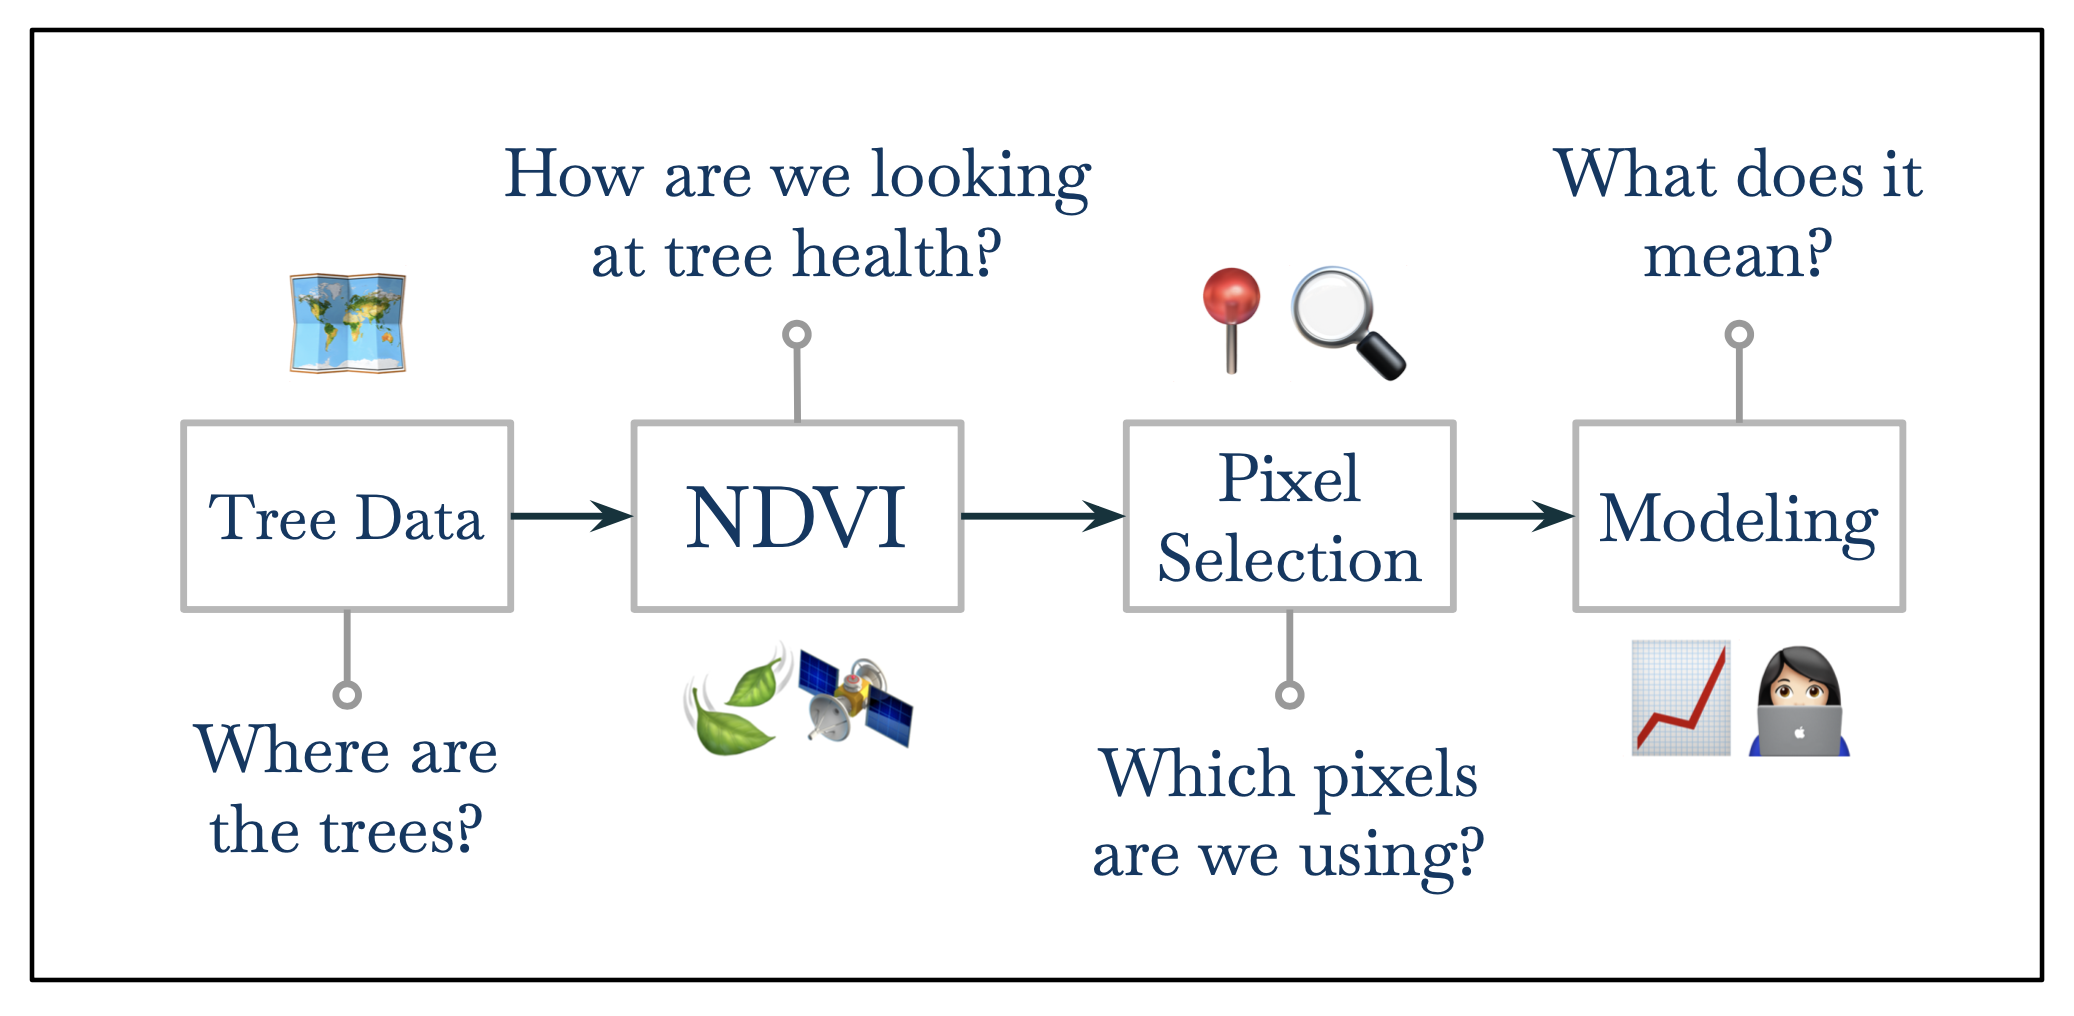
\includegraphics[width=0.95\linewidth,]{figure/methods-overview} 

}

\caption{Overview of methods and data process}\label{fig:methods-overview-fig}
\end{figure}
\hypertarget{previously-collected-field-data}{%
\section{Previously Collected Field Data}\label{previously-collected-field-data}}

As part of a team of researchers, I collected data tree health during
the summer of 2021 as part of the CNH2 Project, which is a larger
collaborative interdisciplinary project examining the relationship
between various socioeconomic variables and urban tree health
({``Smart Trees Collaboratory''} 2022).

For the purposes of the larger project, we selected trees from eight
different neighborhoods in Portland, with four different categorizations
of historic and current investment or disinvestment. The four chosen
species are \emph{Pseudotsuga menziesii, Pinaceae} (PSME), \emph{Thuja plicata,
Cupressaceae} (THPL), \emph{Acer macrophyllum, Sapindaceae} (ACMA), and \emph{Acer
platanoides, Sapindaceae} (ACPL). They are some of the most abundant
tree species in Portland, and make up a large proportion of Portland's
urban forest. PSME, THPL, and ACMA are all native to the area, whereas
Norway Maple is a nonnative tree species that was frequently planted in
residential areas, and is now the most common street tree in Portland.

Individual trees for sampling were selected from the Portland tree
inventories, with the goal of sampling an equal proportion of street
trees and park trees of each species in each neighborhood. Sampling was
also focused on mature trees, so the inventories were filtered to only
include individuals above 25 feet in height. 4 trees of each species
were randomly selected per neighborhood, with an attempt to maintain
equal proportions of park and street trees. However, due to varying
field conditions, some trees were not able to be sampled, so the nearest
tree of the same species that met all criteria was substituted. In
total, 128 trees were surveyed. Fieldwork was conducted between July 7
and August 19, 2021 (Figure \ref{fig:cnh-trees}). Each tree was sampled
in a single visit between 10am and 3pm. Biotic and abiotic variables
were measured, as well as health attributes and physiology of the trees
(Table \ref{tab:var-type-table}). For each tree, a GPS point was
collected to mark its location using ArcGIS Explorer on IOS. Due to the
uncertainty of the GPS points, during post-processing, each collected
tree was matched with the tree location point in the Portland Park and
Street Tree inventories. Any sampled tree points that did not match up
with an inventoried tree point in a margin of 20 feet, it was removed
from further analysis. Any tree individual that did not contain a health
categorization was also removed. The final CNH dataset for my analysis
contained 112 trees (Table \ref{tab:cnh-tree-counts-2}).
\begin{table}

\caption[Final CNH Tree counts]{\label{tab:cnh-tree-counts-2}Counts of species for final CNH tree dataset}
\centering
\begin{tabular}[t]{lllr}
\toprule
Common name & Scientific name & Species code & Number collected\\
\midrule
Bigleaf Maple & Acer macrophyllum & ACMA & 29\\
Norway Maple & Acer platanoides & ACPL & 30\\
Douglas Fir & Pseudotsuga menziesii & PSME & 25\\
Western Redcedar & Thuja plicata & THPL & 28\\
\bottomrule
\end{tabular}
\end{table}
\begin{figure}[H]

{\centering 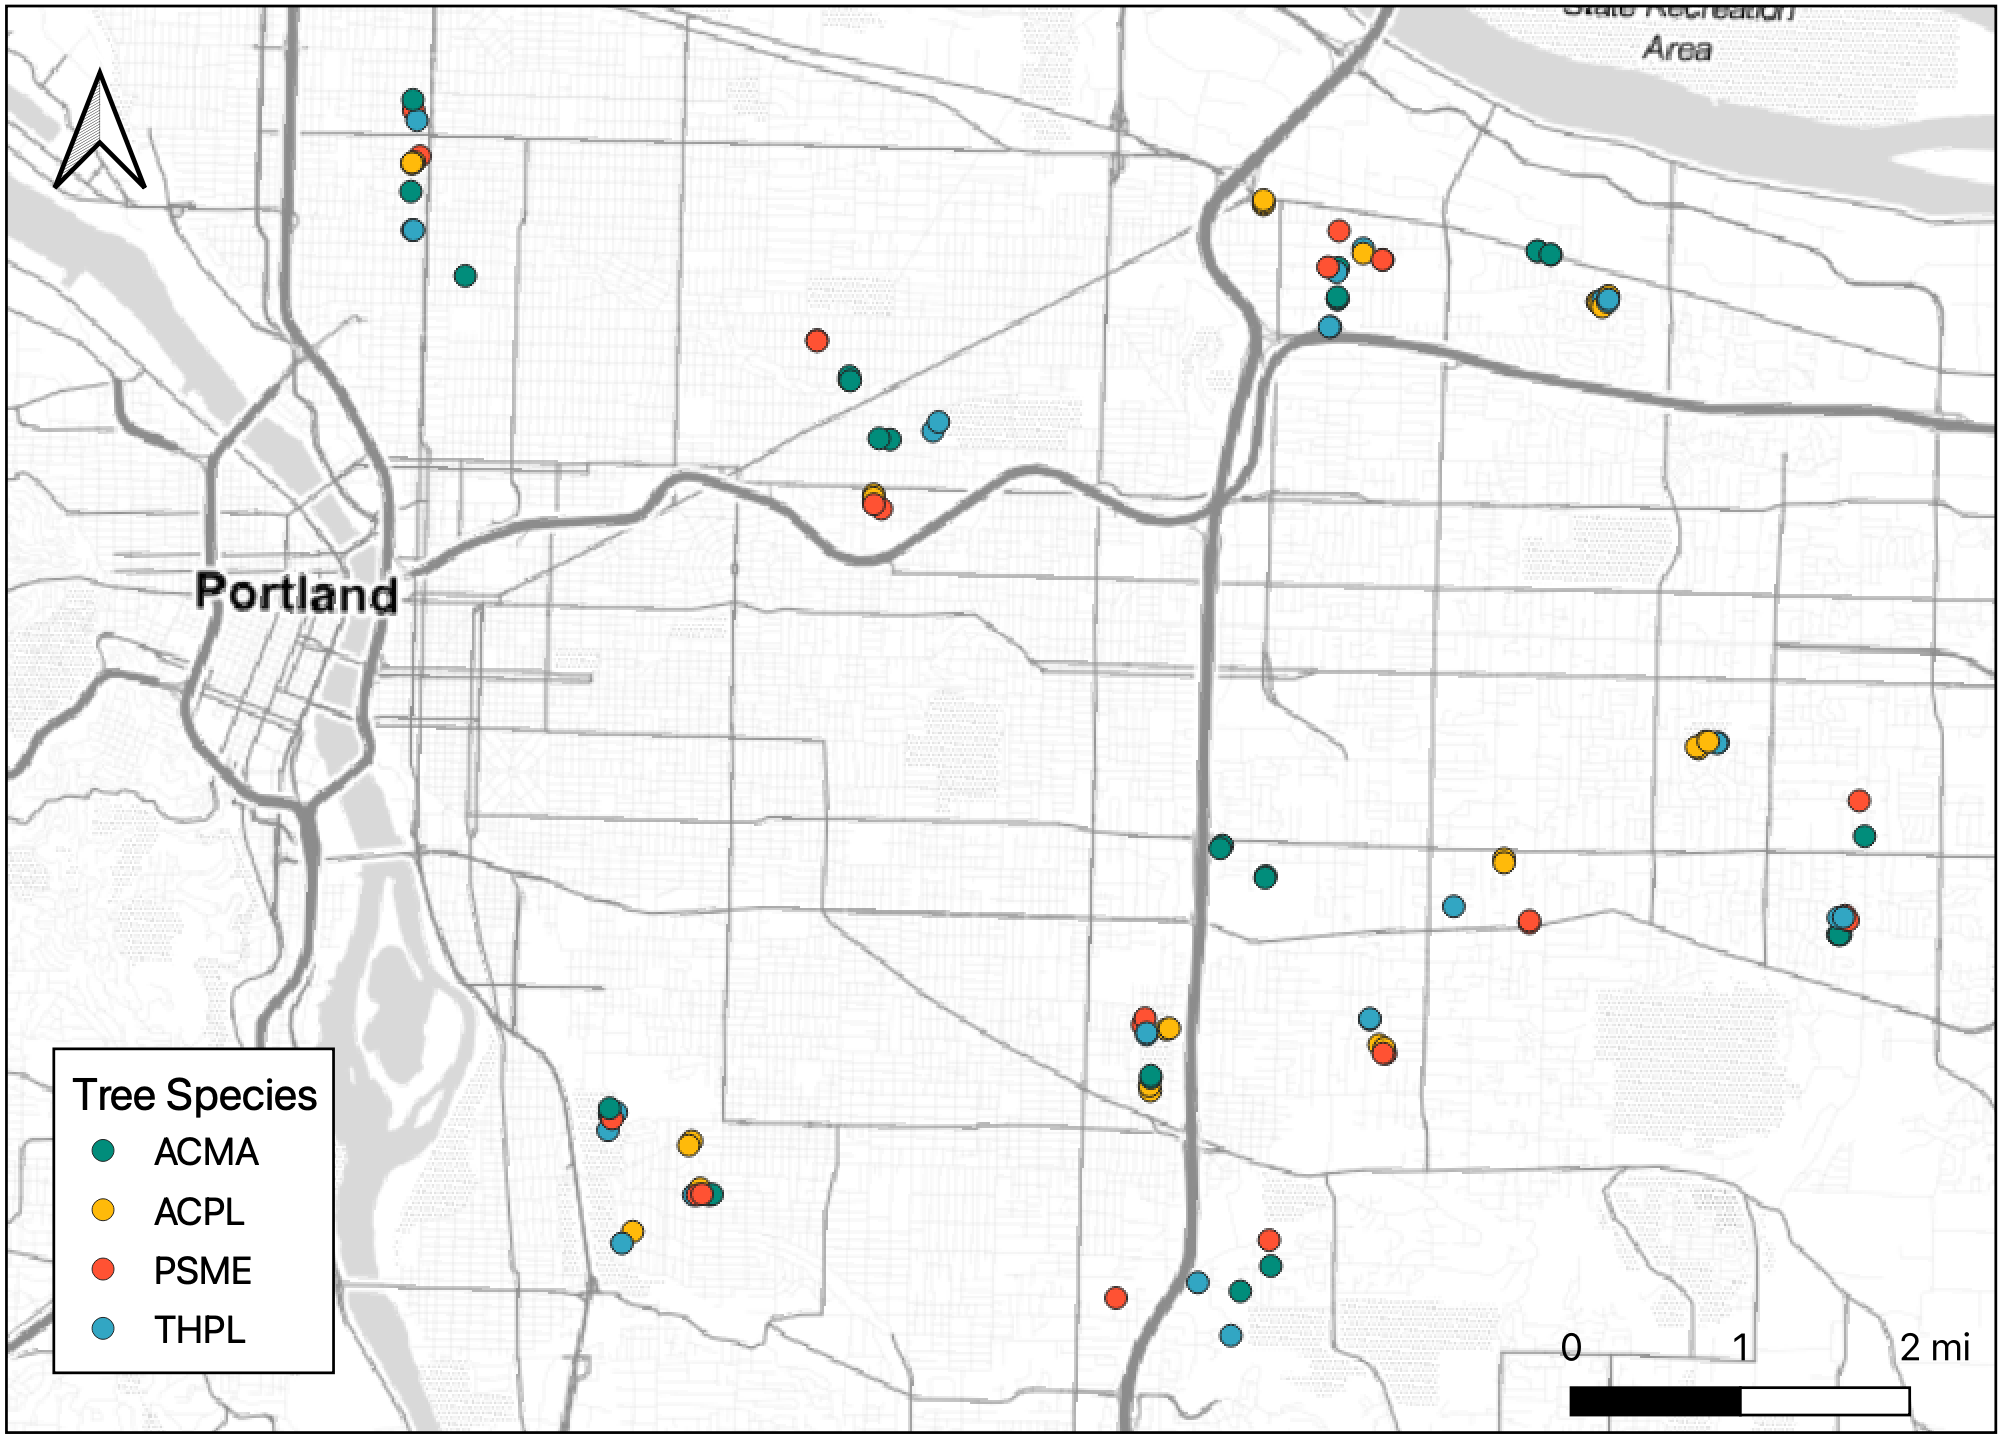
\includegraphics[width=1\linewidth,]{figure/cnh_trees} 

}

\caption{Sampled CNH Trees}\label{fig:cnh-trees}
\end{figure}
\hypertarget{portland-tree-inventory}{%
\section{Portland Tree Inventory}\label{portland-tree-inventory}}

The Portland Tree Inventory Project, managed by the City of Portland's
Parks \& Recreation Urban Forestry Department, cataloged nearly 245,000
street and park trees in Portland between 2010 to 2019. The street tree
inventory, which was collected from 2010 to 2016, contains information
on 216,750 street trees of 145 genera. The park tree inventory,
collected from 2017 to 2019, contains data on 25,740 park trees of 116
genera. While many of the collected variables differ between the two
inventories, they both include data on location, tree identification,
tree diameter at breast height (DBH), and a visual assessment of the
trees health which was rated as \textbf{good}, \textbf{fair}, \textbf{poor}, or dead
(Table \ref{tab:var-type-table}).

To reduce the variability in data due to the time span of data
collection, I filtered the street inventory to trees collected in 2016,
and the park tree inventory to trees that were sampled in 2019. For each
dataset, the selected year was the year with the highest count of trees
sampled, and the trees from 2016 and 2019 were used in my NDVI analysis
and final predictions (Tables \ref{tab:streettable} and
\ref{tab:parktable}) (McConville 2020).
\begin{table}

\caption[Species counts in Street Trees Database]{\label{tab:streettable}Species counts in the Portland Street Trees Database}
\centering
\begin{tabular}[t]{lrr}
\toprule
Species code & Collected in 2016 & Total in inventory\\
\midrule
ACPL & 4373 & 19209\\
THPL & 578 & 1341\\
ACMA & 1306 & 2609\\
PSME & 1254 & 3141\\
\bottomrule
\end{tabular}
\end{table}
\begin{table}

\caption[Species counts in Park Trees Database]{\label{tab:parktable}Species counts in the Portland Park Trees Database}
\centering
\begin{tabular}[t]{lrr}
\toprule
Species code & Collected in 2019 & Total in inventory\\
\midrule
ACPL & 411 & 1502\\
THPL & 331 & 964\\
PSME & 3237 & 6783\\
ACMA & 256 & 490\\
\bottomrule
\end{tabular}
\end{table}
The Portland park and street tree inventories include a health
categorization variable of \textbf{good}, \textbf{fair}, \textbf{poor}, or Dead. A
drawback that can come with qualitative health ratings such as this one
is that if a tree does not appear close to death, or perfectly healthy,
it is very easy to categorize its health as \textbf{fair}, which is what we
see in both the street and park tree databases. The proportion of trees
rated \textbf{fair} is extremely high, especially in the park trees inventory
(Figure \ref{fig:rating-ratios}).
\begin{figure}[H]

{\centering 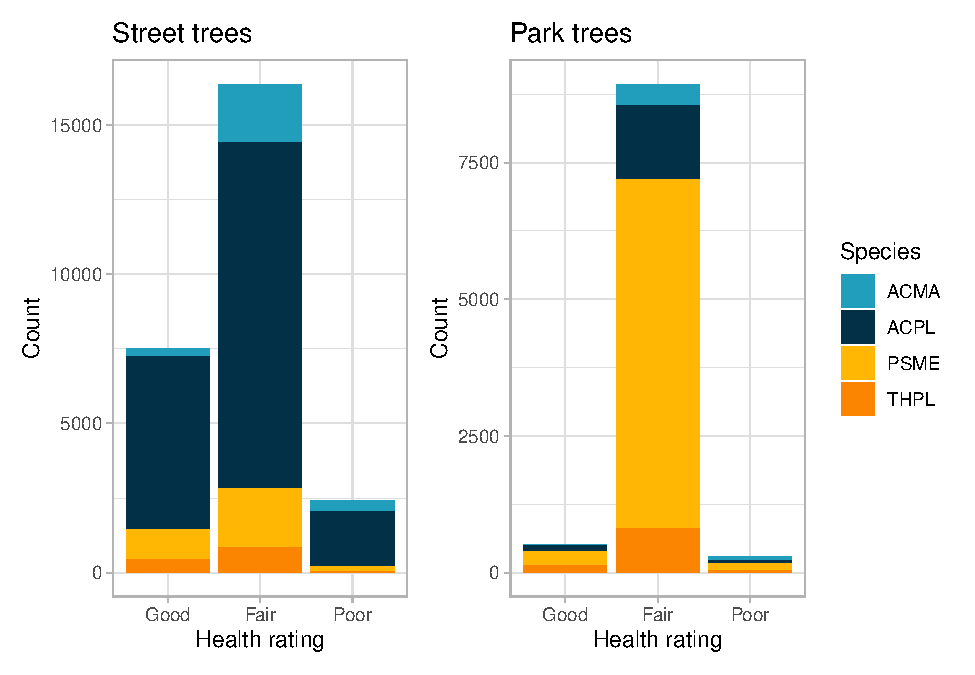
\includegraphics{thesis_files/figure-latex/rating-ratios-1} 

}

\caption{Distribution of Health Ratings in the Portland Tree Inventories}\label{fig:rating-ratios}
\end{figure}
\hypertarget{canopy-width-and-tree-height-model}{%
\subsection{Canopy width and tree height model}\label{canopy-width-and-tree-height-model}}

The park tree dataset contains measurements for tree height, canopy
width, and DBH, but the street tree dataset only contains measurements
for DBH. In order to successfully filter out all trees shorter than 25
feet tall, a height measurement is necessary. Canopy width is an
essential factor of the radius pixel selection method, which is
discussed below (section \ref{radiusmethod}). Using RStudio, I created
a statistical model to predict tree height and crown width based on tree
DBH and species in order to be able to use the same pixel selection
methods for both the park and street tree inventories (section
\ref{canopy-model-results}).

\hypertarget{satellite-imagery}{%
\section{Satellite Imagery}\label{satellite-imagery}}

The multispectral satellite imagery used in this thesis was accessed
through Planet Labs Education and Research Program, which provides
limited non-commercial access to PlanetScope satellite imagery for those
with a college or university email address. The available imagery had a
pixel resolution of 3 meters, and a 4-band product (RGB-NIR). The bands
in a satellite product refer to the reflectance wavelength that is
picked up by the satellite. For a 4-band satellite product, the
wavelengths are split into red, green, blue, and near-infrared (NIR)
bands (Table \ref{tab:wavelength}). In the raw PlanetScope product,
these 4 bands come compressed in one \texttt{.tif} image.
\begin{longtable}[t]{ll}
\caption[4-band satellite wavelength ranges]{\label{tab:wavelength}Wavelength ranges for 4-band Planetscope satellite bands}\\
\toprule
Band name & Wavelength range\\
\midrule
Blue & 455 - 515 nm\\
Green & 500 - 590 nm\\
Red & 590 - 670 nm\\
NIR & 780 - 860 nm\\
\bottomrule
\end{longtable}
PlanetScope satellite imagery (Planet Labs, 3m resolution, 4-band
RGB-NIR) was used for vegetation index calculation. PlanetScope, also
known as the Flock, is a constellation of approximately 130 satellites .
The first 28 PlanetScope satellites were launched in July 2014, and the
newest batch of satellites were launched in January 2022. PlanetScope,
operated by Planet, is a constellation of approximately 130 satellites,
able to image the entire land surface of the Earth every day (a daily
collection capacity of 200 million km\(^2\)/day). PlanetScope images are
approximately 3 meters per pixel resolution ({``Planet Imagery Product Specifications''} 2022). A
downloaded satellite product for an area of interest is comprised of
multiple scene products. Each scene product is an individual image of a
swath of land that is at least partially contained within the area of
interest. (Figures \ref{fig:2016-swath}, \ref{fig:2019-swath},
\ref{fig:2021-swath}).

I downloaded satellite images corresponding to the summers of when the
data was collected (2016, 2019, and 2021). Images were first filtered
for those captured in July of each year, since images taken during the
middle of the on-leaf period have been shown to be most sensitive in
detecting a statistical difference in tree health measured by NDVI
(Fang et al. 2020). The remaining images were then filtered for minimal cloud
cover and maximum coverage of the area of study. The final selected
images were taken between 6:30 and 7pm on 6 July 2016, 31 July 2019, and
26 July 2021 (Table \ref{tab:sat-products}).
\begin{longtable}[t]{llrl}
\caption[Satellite product specifications]{\label{tab:sat-products}Satellite product specifications for PlanetScope multispectral satellite image products}\\
\toprule
Collection date & Collection time & Number of scene products & Satellite ID\\
\midrule
2016-07-06 & 18:55 & 5 & 0c22\\
2019-07-31 & 18:42 & 4 & 0f42\\
2021-07-26 & 18:40 & 4 & 1003\\
\bottomrule
\end{longtable}
For each of the chosen dates, I downloaded the available analytic
product from Planet. The analytic multispectral imagery products are
orthorectified, calibrated, corrected for terrain distortions, and
transformed to Top of Atmosphere radiance to ensure accurate geolocation
and cartographic projection.

\hypertarget{ndvi-calc-methods}{%
\section{NDVI calculation}\label{ndvi-calc-methods}}

The NDVI calculations were done using Python in PyCharm. Besides minor
alterations, the processing code came from Planet's instructions on
calculating NDVI from 4-band PlanetScope data (Planet, n.d.). NDVI is
calculated from the red and NIR satellite bands, as shown in Equation
\eqref{eq:ndvi-eq}. NDVI is calculated for each individual pixel of the
satellite image.
\begin{equation}
  \mathrm{NDVI} = \frac{(NIR - Red)}{(NIR + Red)} 
  \label{eq:ndvi-eq}
\end{equation}
\begin{figure}[H]

{\centering 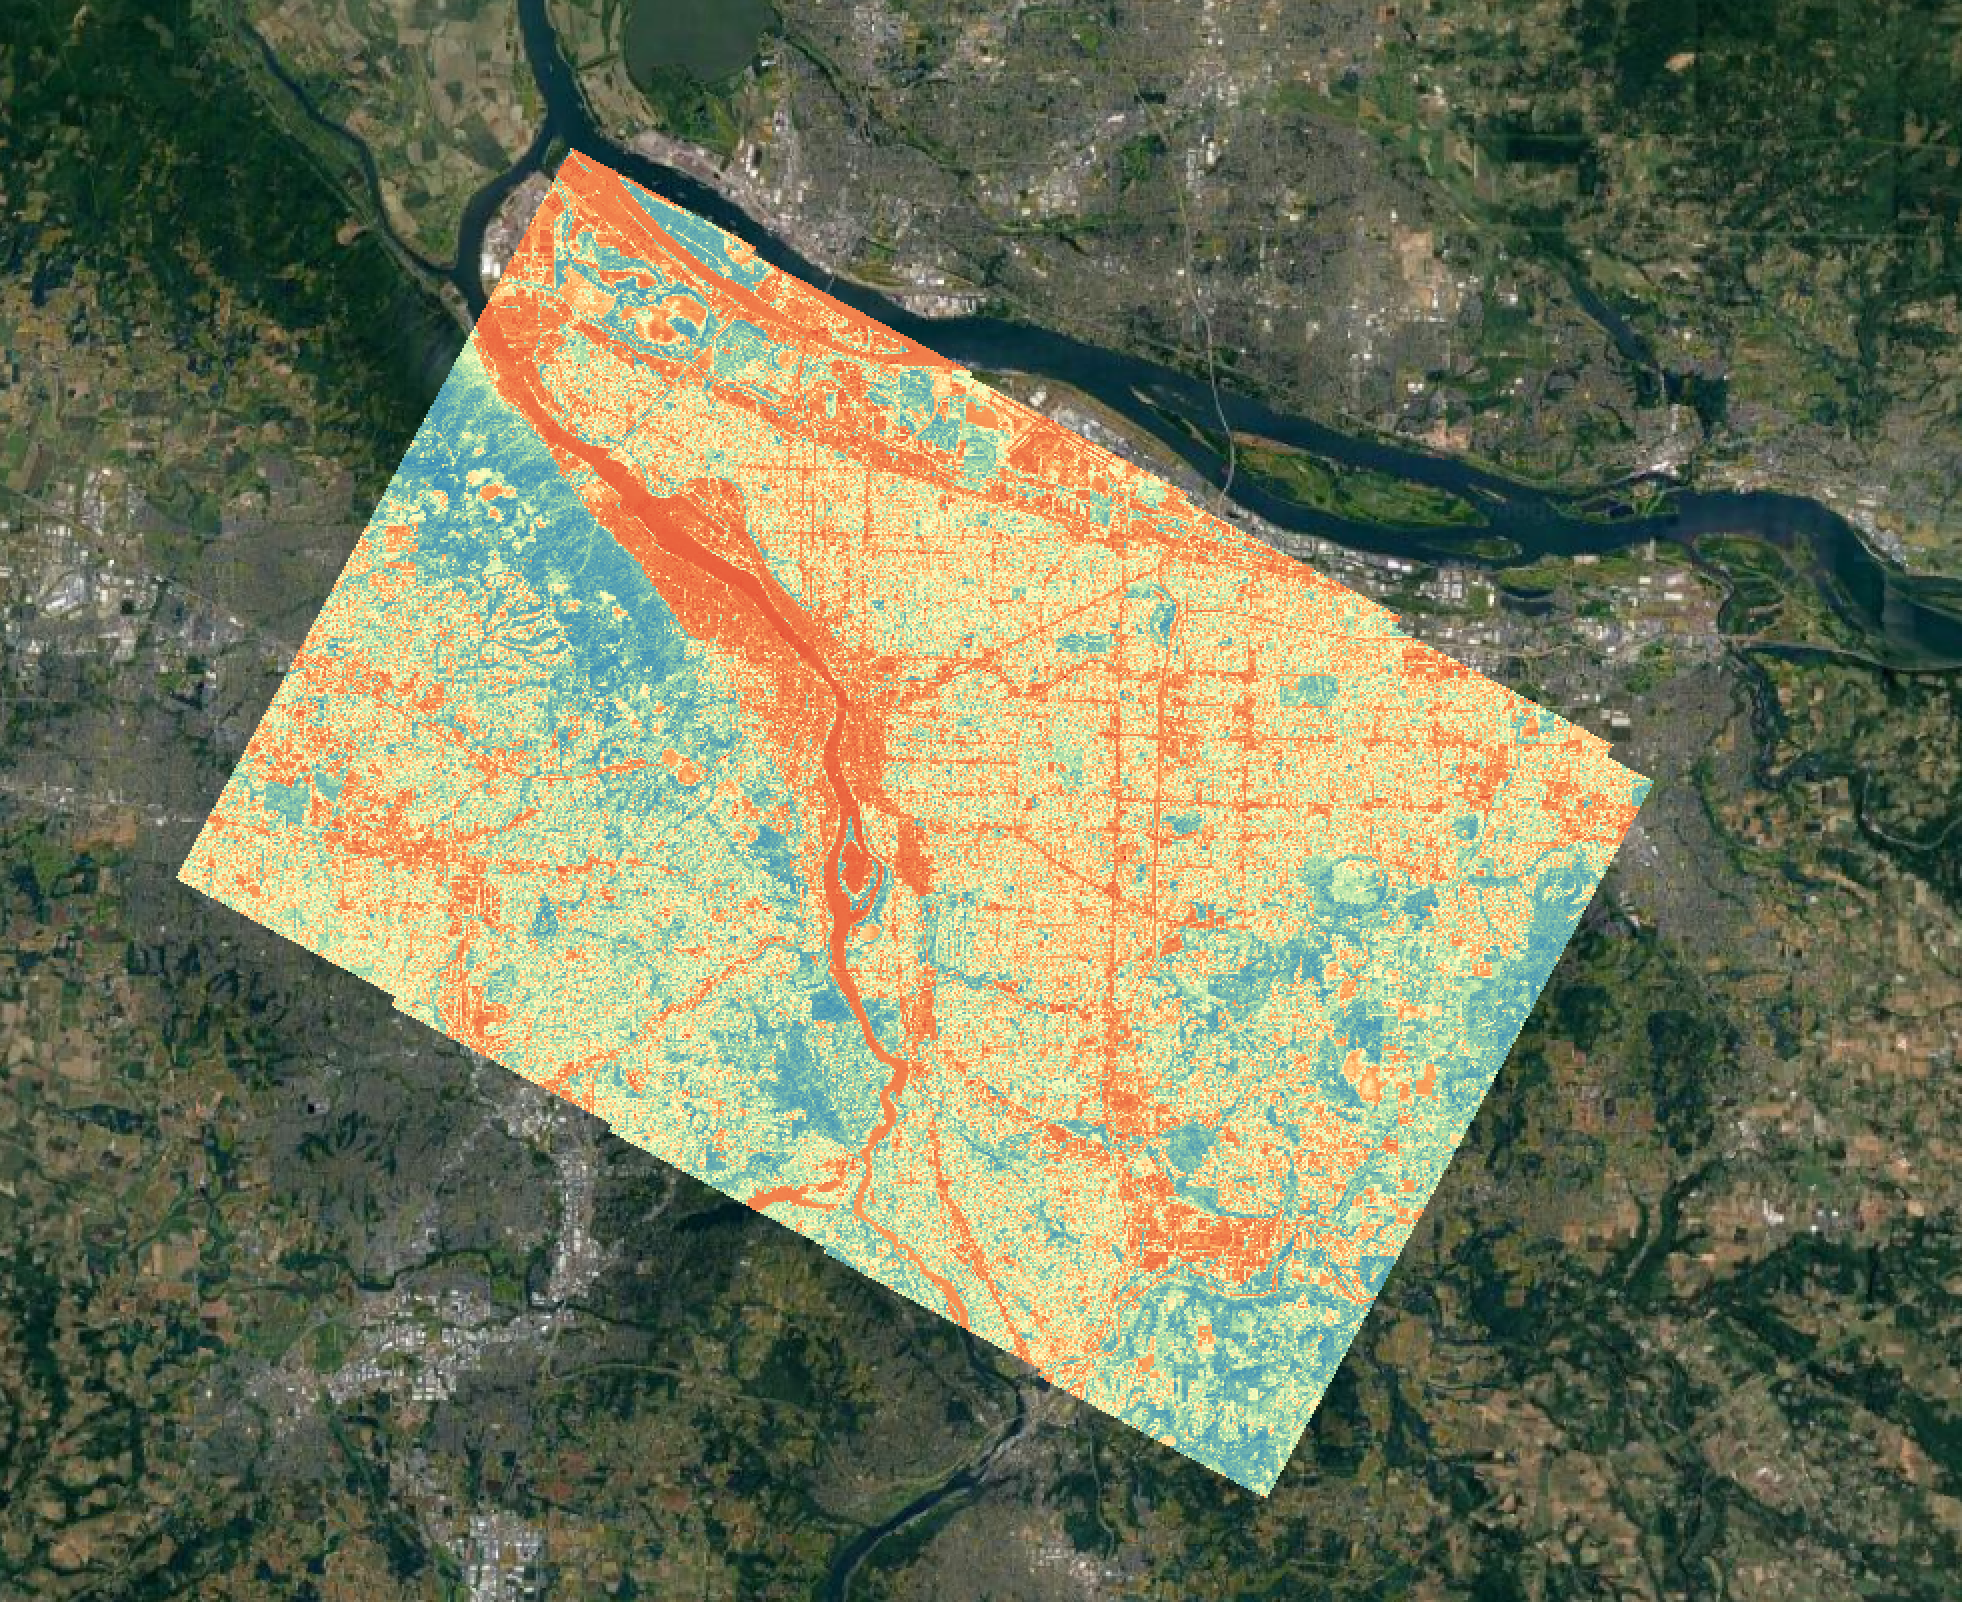
\includegraphics[width=0.32\linewidth,]{figure/2016_ndvi} 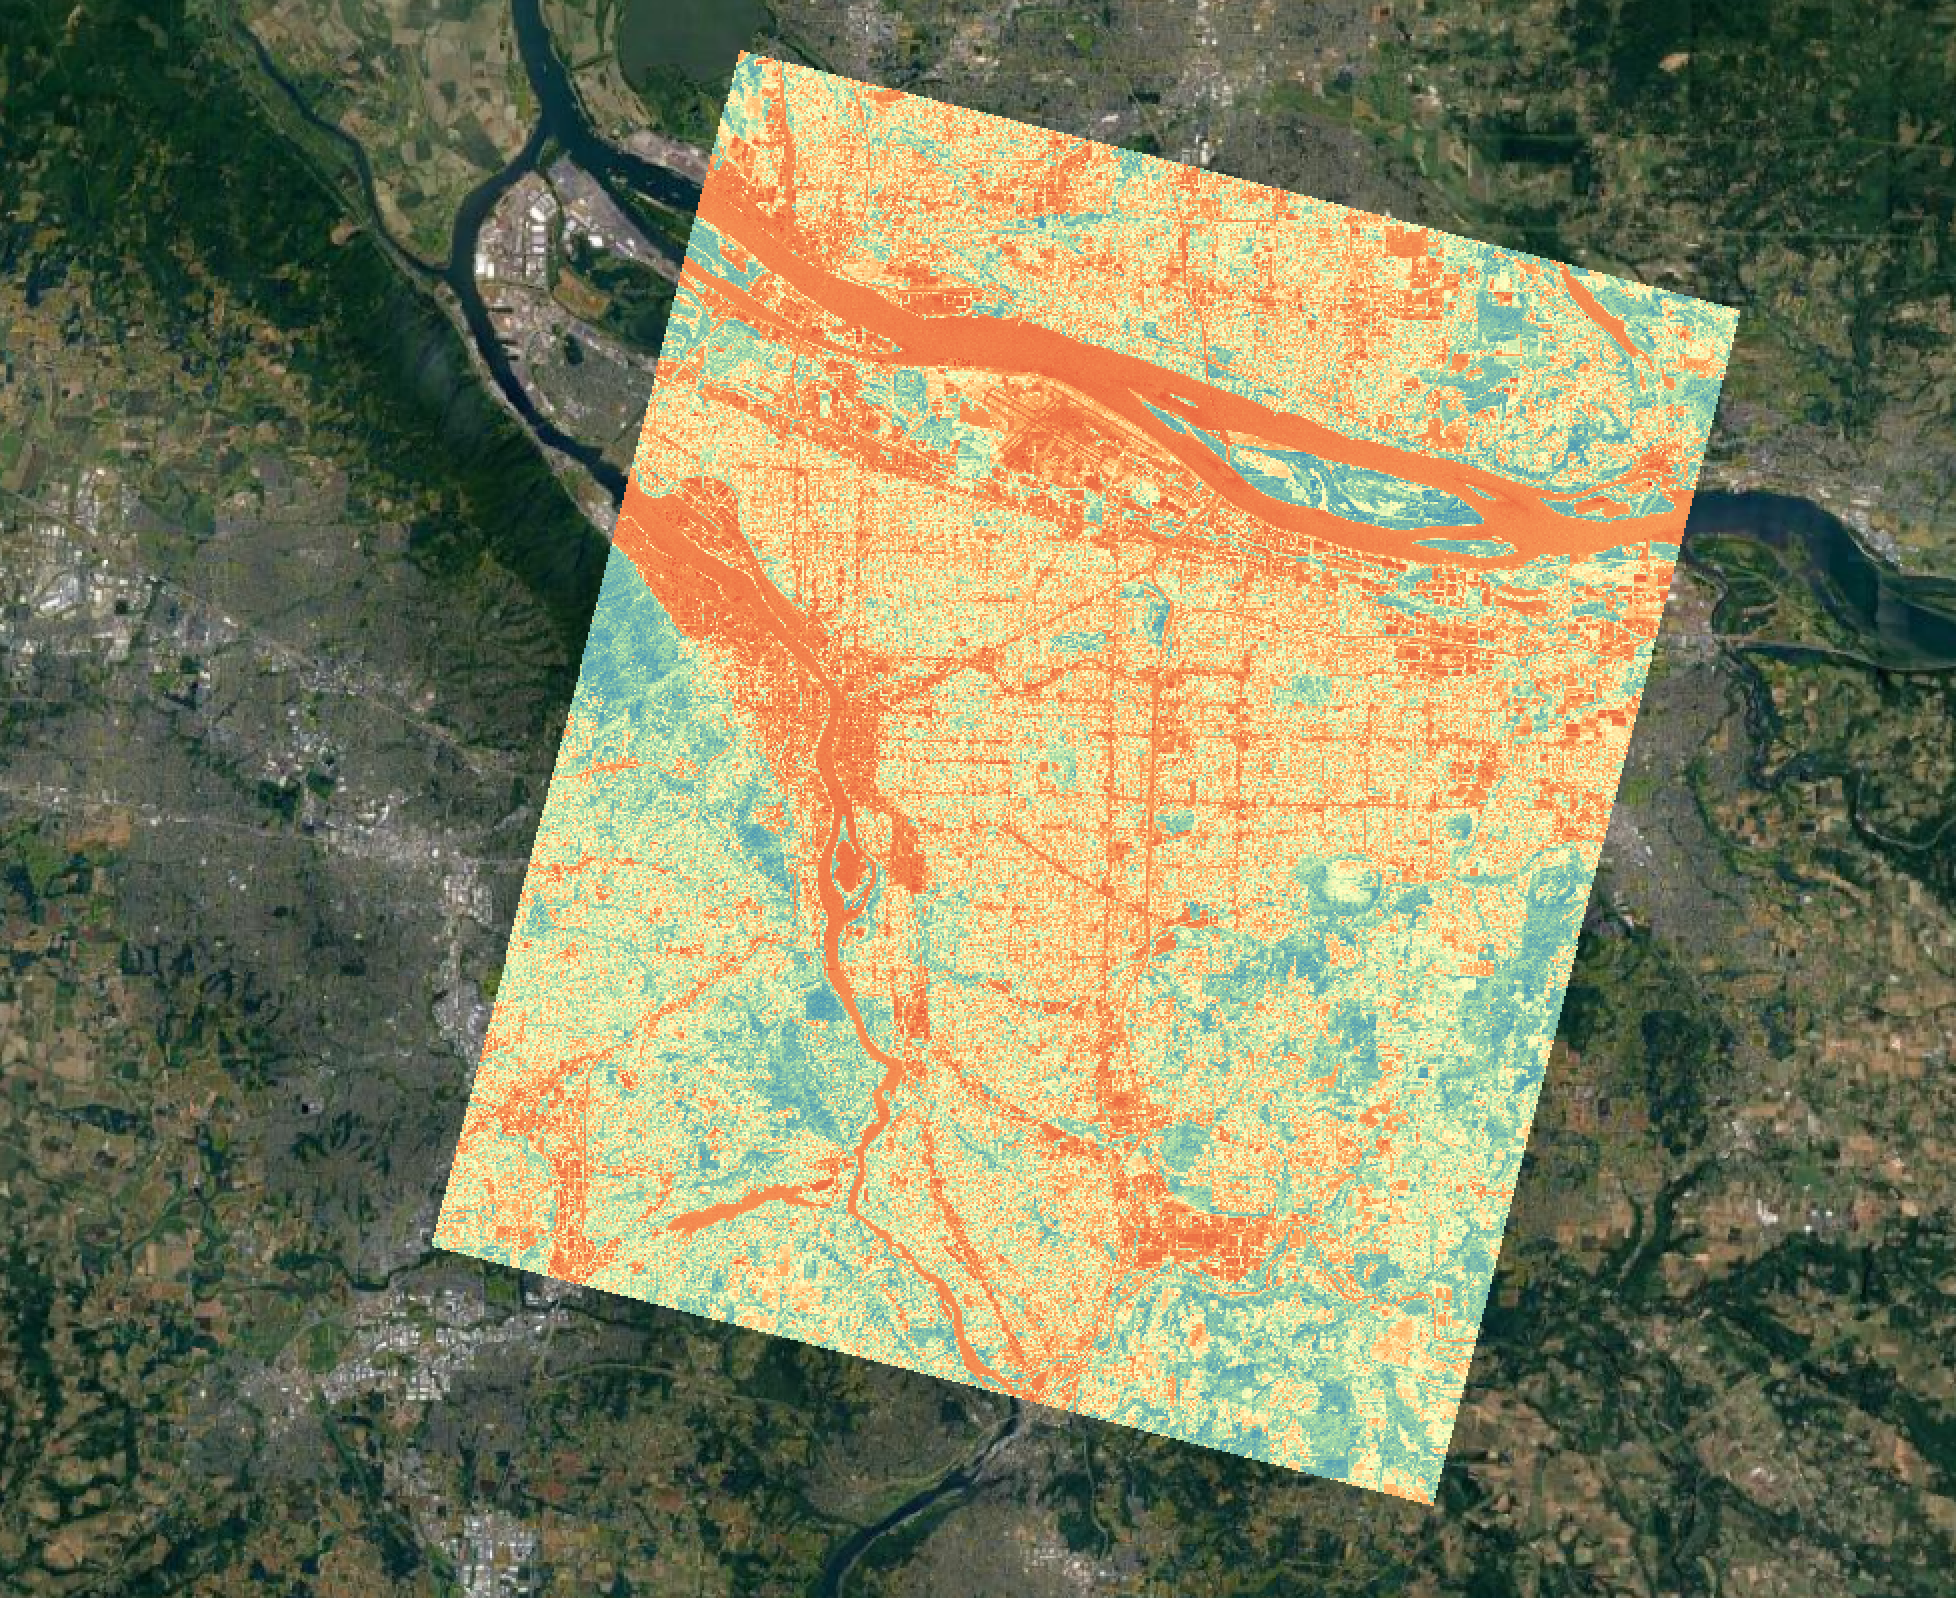
\includegraphics[width=0.32\linewidth,]{figure/2019_ndvi} 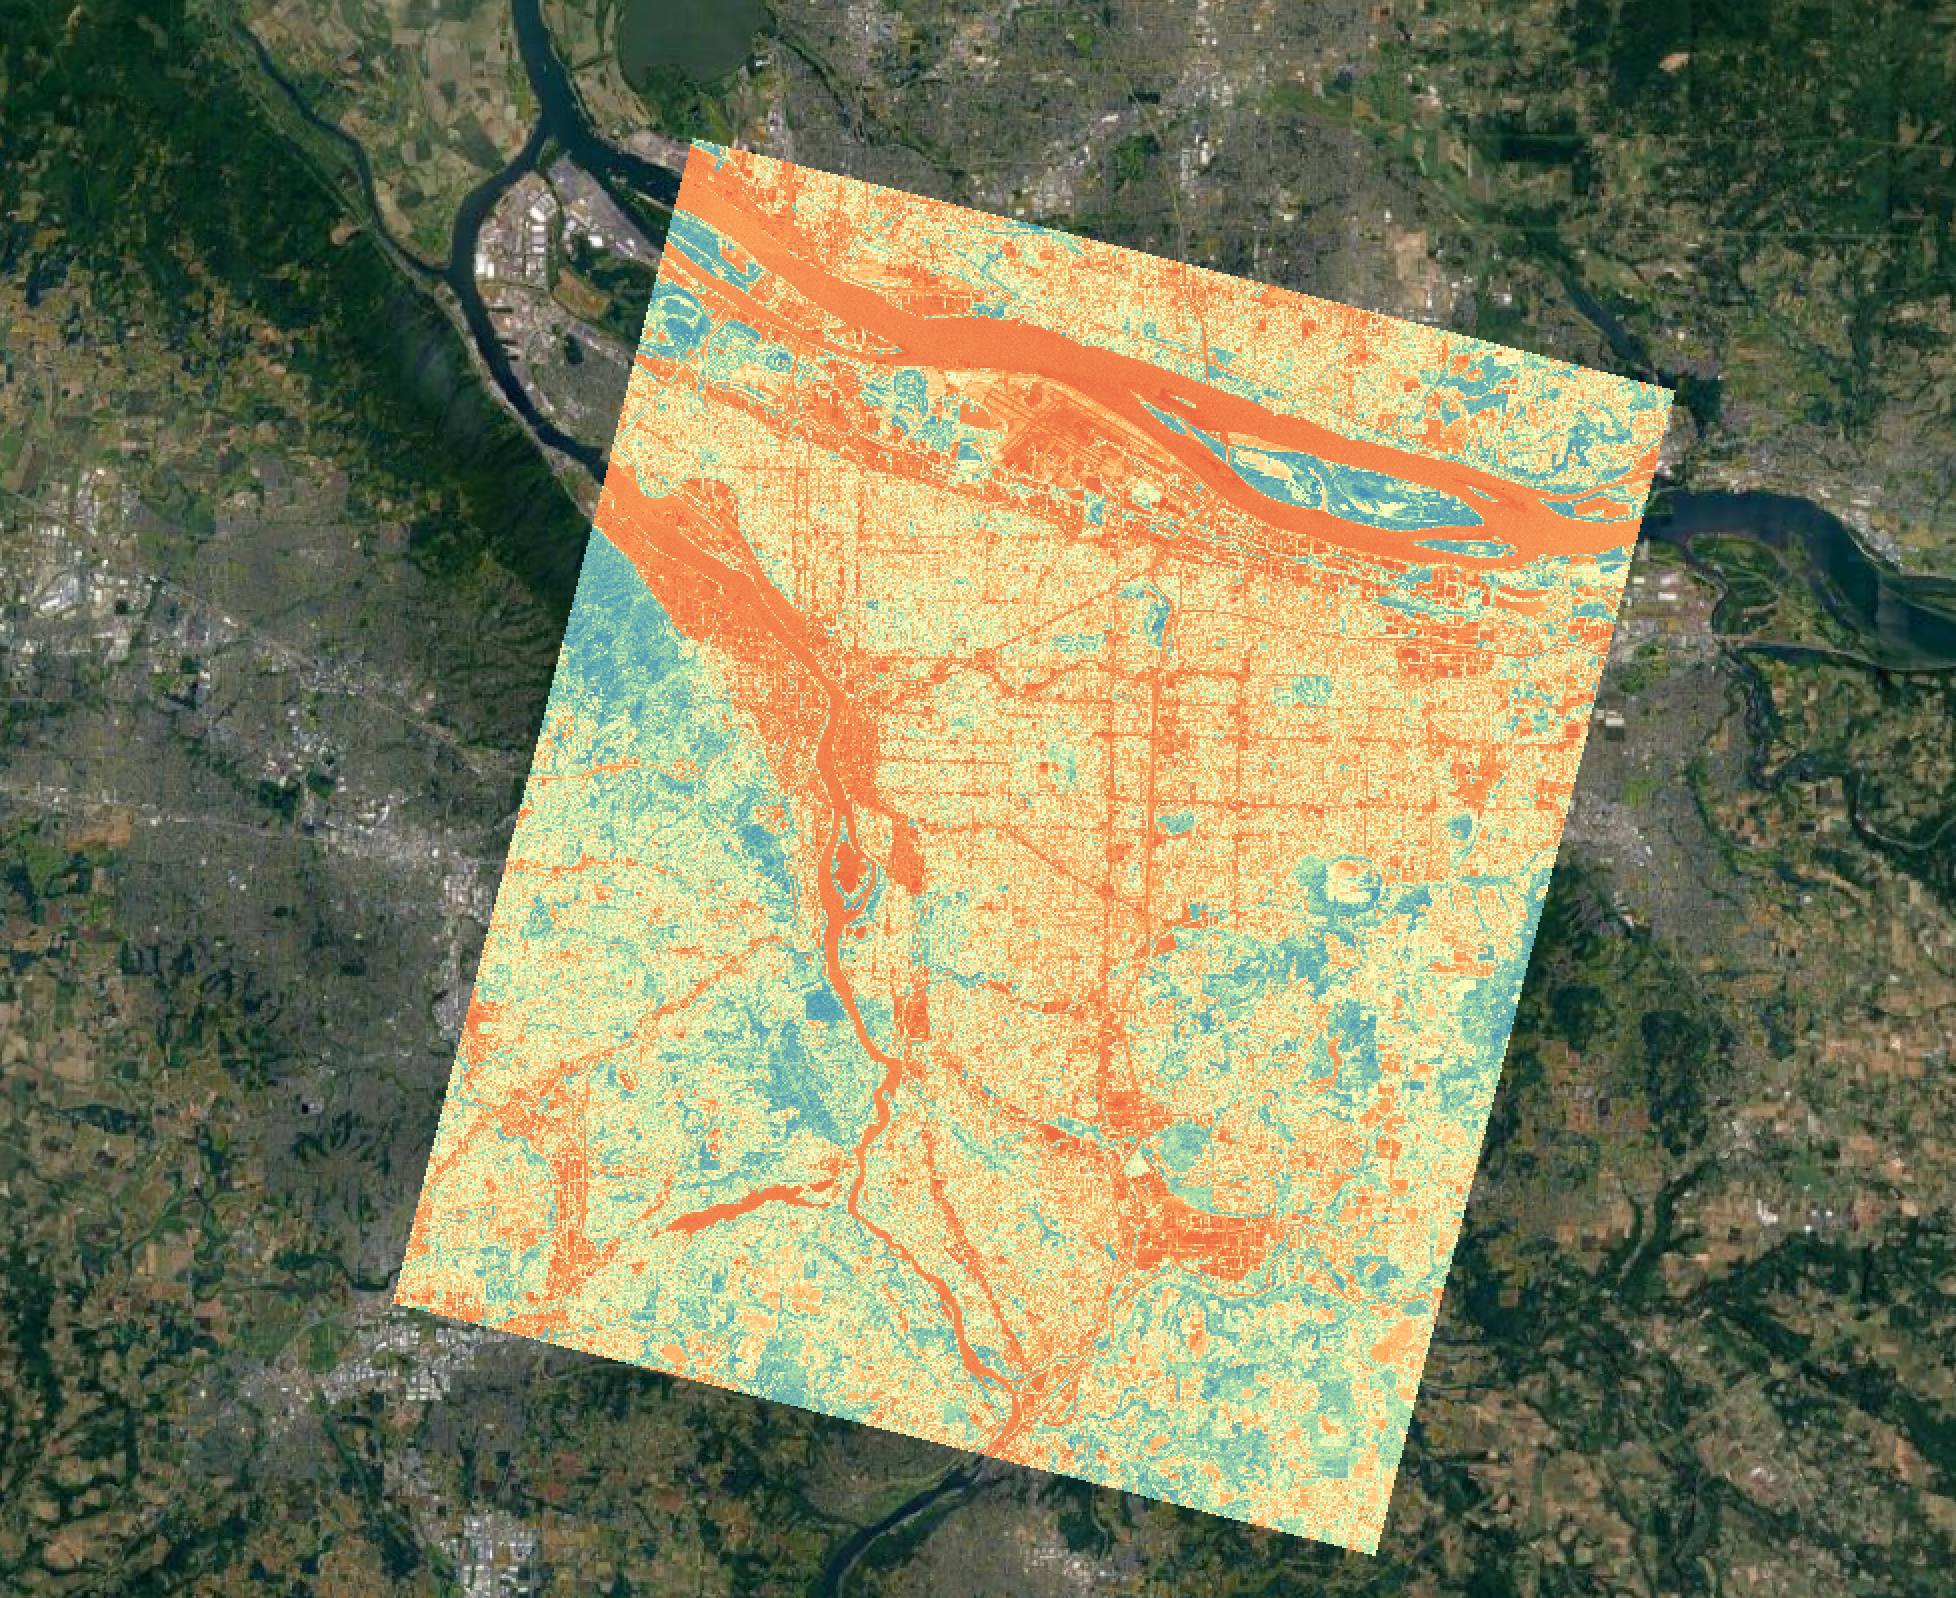
\includegraphics[width=0.32\linewidth,]{figure/2021_ndvi} 

}

\caption{Product areas for 2016, 2019, and 2021 satellite scenes}\label{fig:areafigs}
\end{figure}
\hypertarget{chm}{%
\section{Canopy Height Model}\label{chm}}

A canopy height model for the Portland metro area was developed using
LiDAR and satellite spectral imagery collected in the summer of 2014
({``Canopy 2014''} 2016). The purpose of this data is to monitor natural areas in
the Portland metro area, specifically change over time analysis and the
examination of the potential loss of habitat in riparian areas. The
canopy was detected using both NDVI values and LiDAR feature heights.
Errors and noise in the data, such as electrical lines above tree tops,
were cleaned using geometric post-processing. The canopy height model
was clipped to remove anything below ten feet to eliminate any
understory shrubs or grasses that were included in the raw data
({``Canopy 2014''} 2016).

\hypertarget{tree-crown-delineation-and-pixel-selection}{%
\section{Tree Crown Delineation and Pixel Selection}\label{tree-crown-delineation-and-pixel-selection}}

The goal of tree crown delineation is to understand where the foliage of
a tree is located. This is extremely important because we want to ensure
that the satellite pixels used for health analysis have measurements
that belong to the given tree. Previous papers such as have used manual
tree crown delineation (Xiao et al. 2005), or chosen a standardized radius for
all trees in their sample (Fang et al. 2020). Manual tree crown delineation
would be extremely time consuming, especially when trying to examine
data on a city-wide level. Additionally, with a standardized radius,
there will be many trees that have crowns either larger or smaller than
the standardized radius. If the true crown is smaller than that of the
radius, pixels that correspond to things like grass or pavement will be
included in the measurement analysis. Conversely, if the true crown is
larger than the chosen radius, the edges of the tree will be ignored,
and valuable data will be lost. With both of these methods, any
overlapping tree crowns were removed from the final analysis, even
further reducing the sample size.

In this thesis, I test three different methods of pixel selection for
NDVI analysis. First, I test a ``point method'' which uses the NDVI value
from a single pixel directly below an inventoried trees location point.
Second, I use crown width measurements and predictions to create a
variable radius method, and average the NDVI pixels within the created
circle. Lastly, I use a LiDAR created canopy height model for Portland's
urban canopy with \texttt{ForestTools} canopy delineation algorithm to create
canopy polygons for NDVI analysis (Plowright et al. 2021).

For the following examples, I use Berkeley Park, located in SE Portland,
to demonstrate the different delineation techniques. We sampled 6 CNH
trees in Berkeley Park: 2 Bigleaf Maple, 1 Norway Maple, 2 Douglas Fir,
and 1 Western Redcedar (Figure \ref{fig:berkeley-park}).
\begin{figure}[H]

{\centering 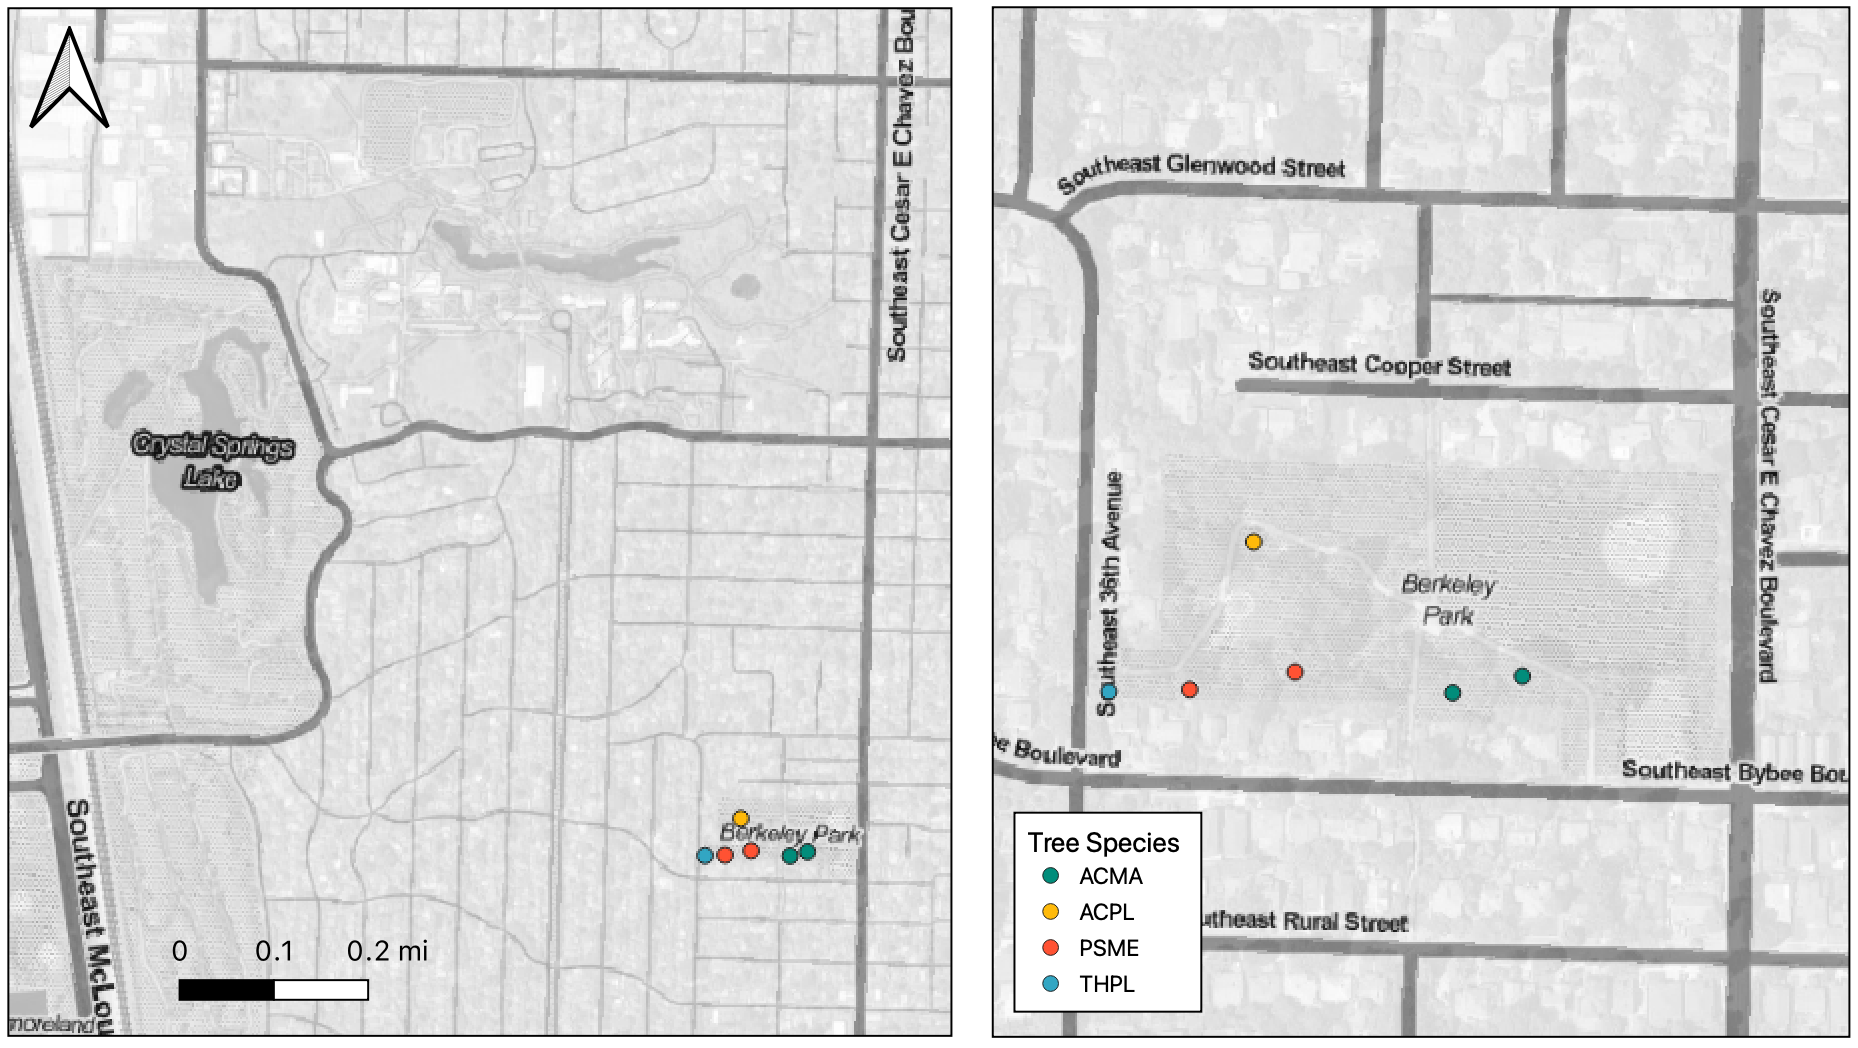
\includegraphics[width=1\linewidth,]{figure/berkeley_park} 

}

\caption{Berkeley Park and CNH trees}\label{fig:berkeley-park}
\end{figure}
\hypertarget{point-method}{%
\subsection{Point method}\label{point-method}}

For the point method, I extracted the NDVI value from the
pixel directly underneath the tree location point. This is the simplest
of the three methods, since it obtains one NDVI value for one singular
pixel. The tree location points were sourced from the street and park
tree inventories and processed in QGIS (Figure \ref{fig:point-method}).
The main source of potential error with this technique is with the tree
point location. If the point was placed incorrectly, the NDVI value will
not be representative of the tree's greenness, or health.
\begin{figure}[H]

{\centering 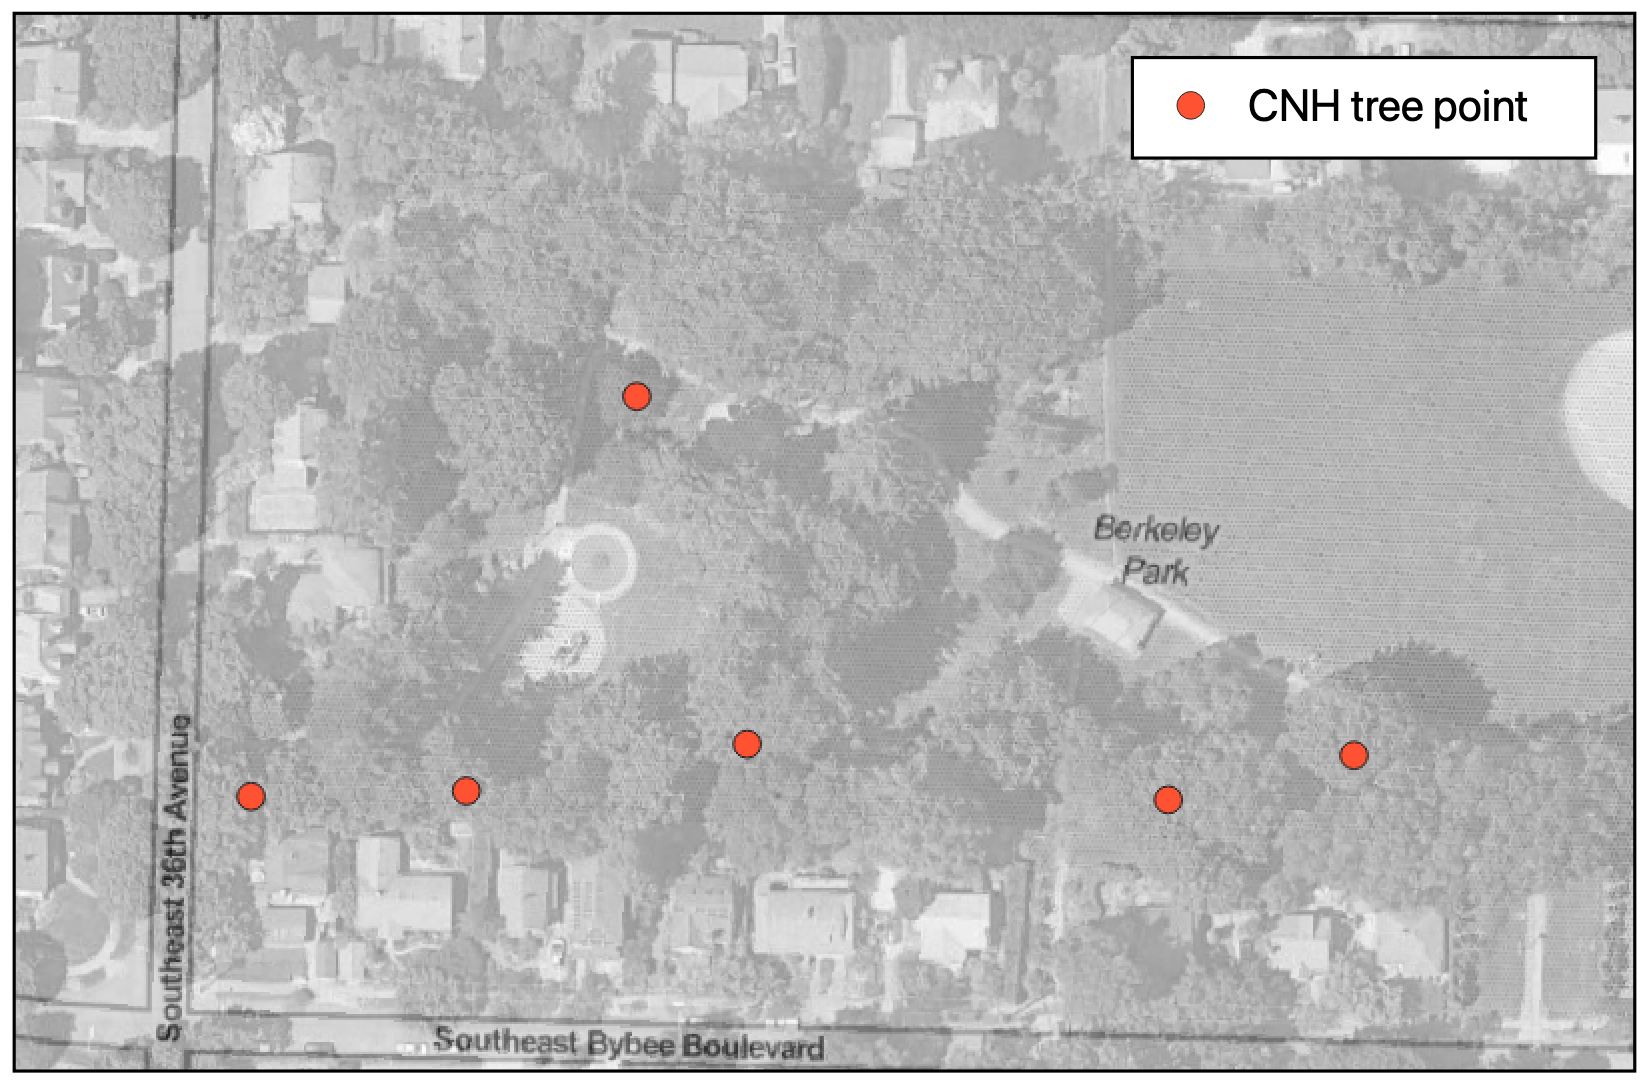
\includegraphics[width=0.8\linewidth,]{figure/points} 

}

\caption{CNH trees sampled in Berkeley Park}\label{fig:point-method}
\end{figure}
\hypertarget{radiusmethod}{%
\subsection{Radius method}\label{radiusmethod}}

The first method of tree crown delineation I used is based on the
individual crown width for each selected tree. In the Portland park tree
inventory, crown width is measured as an east to west diameter, and a
north to south diameter. To get the radius for the buffer, I took the
average of both measurements and divided it by 2. For the Portland
street tree inventory, crown width was not collected. I used the tree
height and crown width predictive model to create crown width
measurements. For each selected tree point, I created a buffer with the
radius of the measured or predicted tree canopy using QGIS (Figure
\ref{fig:point-radius}). To get NDVI for each tree in this method, I
averaged the value of all pixels in the buffer circle for each tree
using QGIS.

With the radius method, it involves the same risk as the point method
that if the central point is incorrectly located, the values will not be
representative. Additionally, average NDVI ratings obtained with this
method for trees with overlapping crowns will contain NDVI pixels that
belong to other trees. Previous studies have removed all overlapping
tree crowns when using a radius technique, but that can severely limit
sample size of available data for analysis, since especially in urban
areas and on streets, most of the trees will have overlapping crowns.
\begin{figure}[H]

{\centering 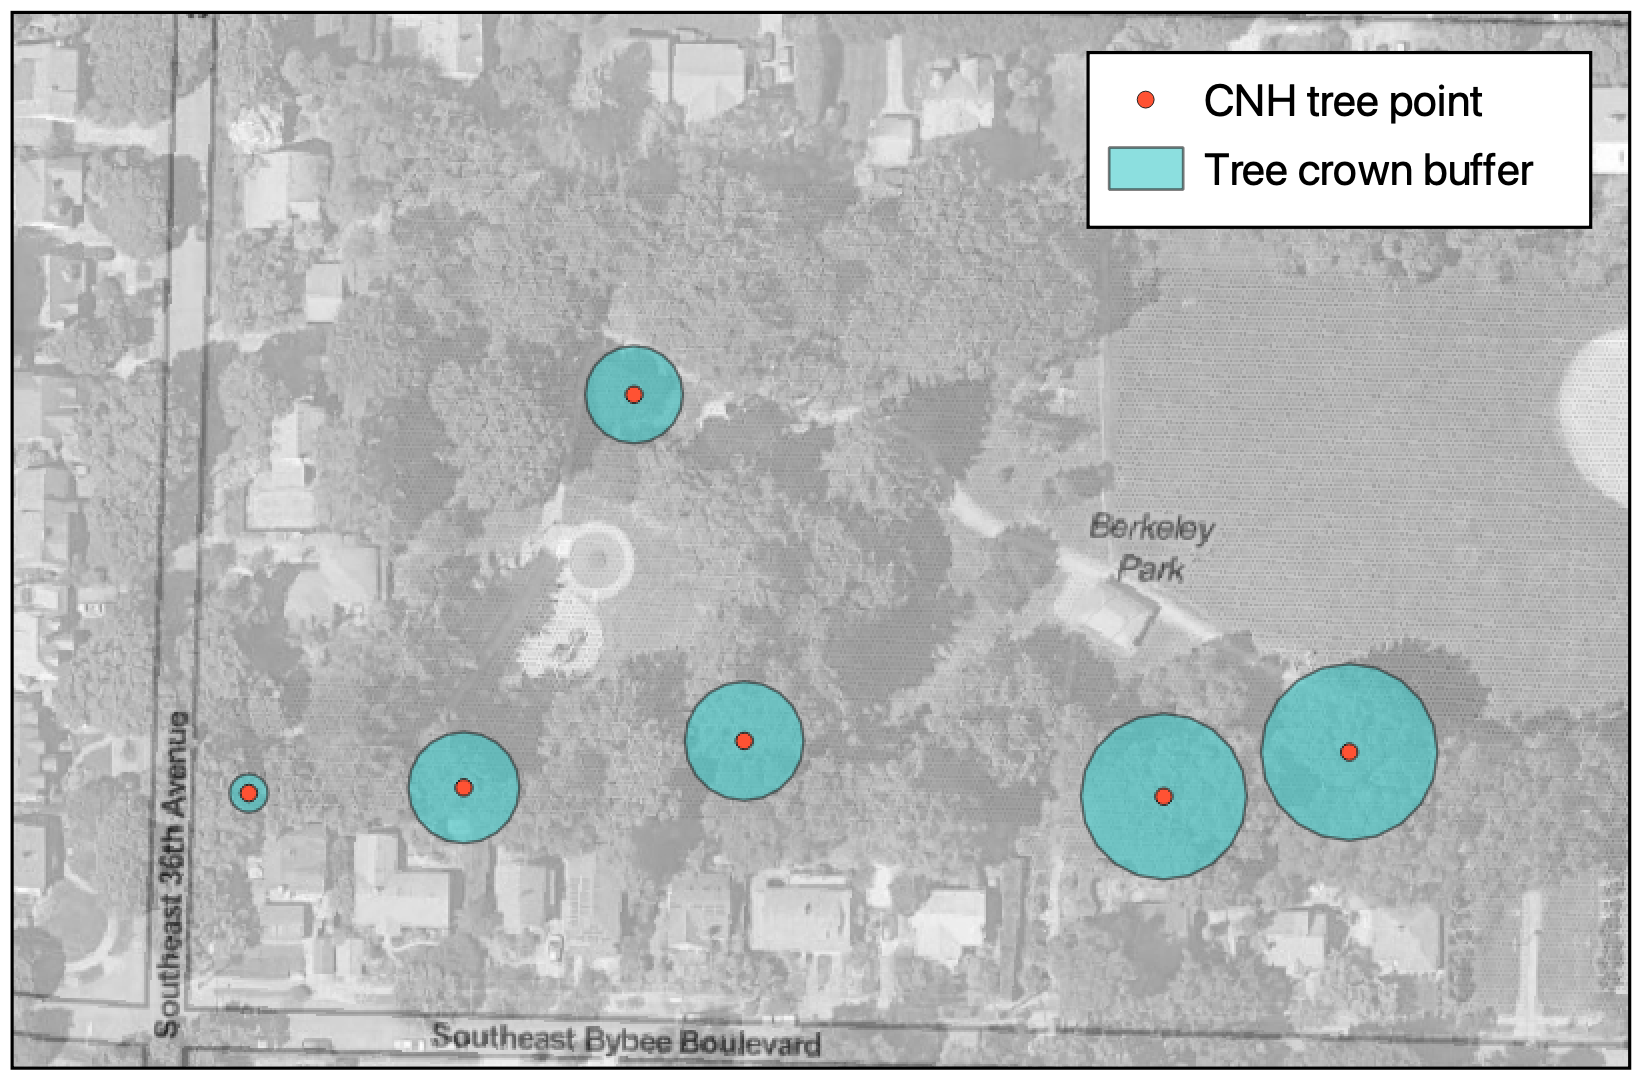
\includegraphics[width=0.8\linewidth,]{figure/point_radius} 

}

\caption{CNH trees with crown width buffer}\label{fig:point-radius}
\end{figure}
\hypertarget{lidar-method}{%
\subsection{LiDAR method}\label{lidar-method}}

The LiDAR method is the most complex and involved of the three tree
crown delineation methods but has the potential to be the most precise.

The \texttt{ForestTools} crown delineation algorithm is a modified watershed
delineation algorithm that takes a LiDAR file input, as well as treetop
location point file and outputs a polygon file with predicted tree
crowns. \texttt{ForestTools} also has the ability to predict treetop location
points based on LiDAR data, but that functionality introduced a lot of
error in my processing because it became difficult to re-associate
predicted treetop points with the actual tree location points that I was
analyzing.

The LiDAR canopy height model was clipped to a 30 meter buffer around
each selected tree point to reduce file size in the delineation
processing (Figure \ref{fig:lidar-buffer}). A 30m buffer was chosen to
ensure that no part of the tree canopy would be omitted from the
processing, and to include any near neighboring trees that may have
canopy that overlaps with the tree of interest. In order for the
algorithm to delineate tree crowns, it needs both LiDAR canopy data and
location points for the potential trees for delineation. With a smaller
buffer radius, the locations of neighboring trees would be omitted and
the canopy delineation algorithm would compute a tree crown as much
bigger than it actually is.

With the 30m buffer, all other inventoried trees that are contained
within the buffer were selected for inclusion as treetop location points
in addition to the trees of interest (Figure \ref{fig:buffer-points}).
A minimum tree height of 20 feet was included in the algorithm options
but since all sampled trees were already filtered for height
requirements, this may not be necessary.
\begin{figure}[H]

{\centering 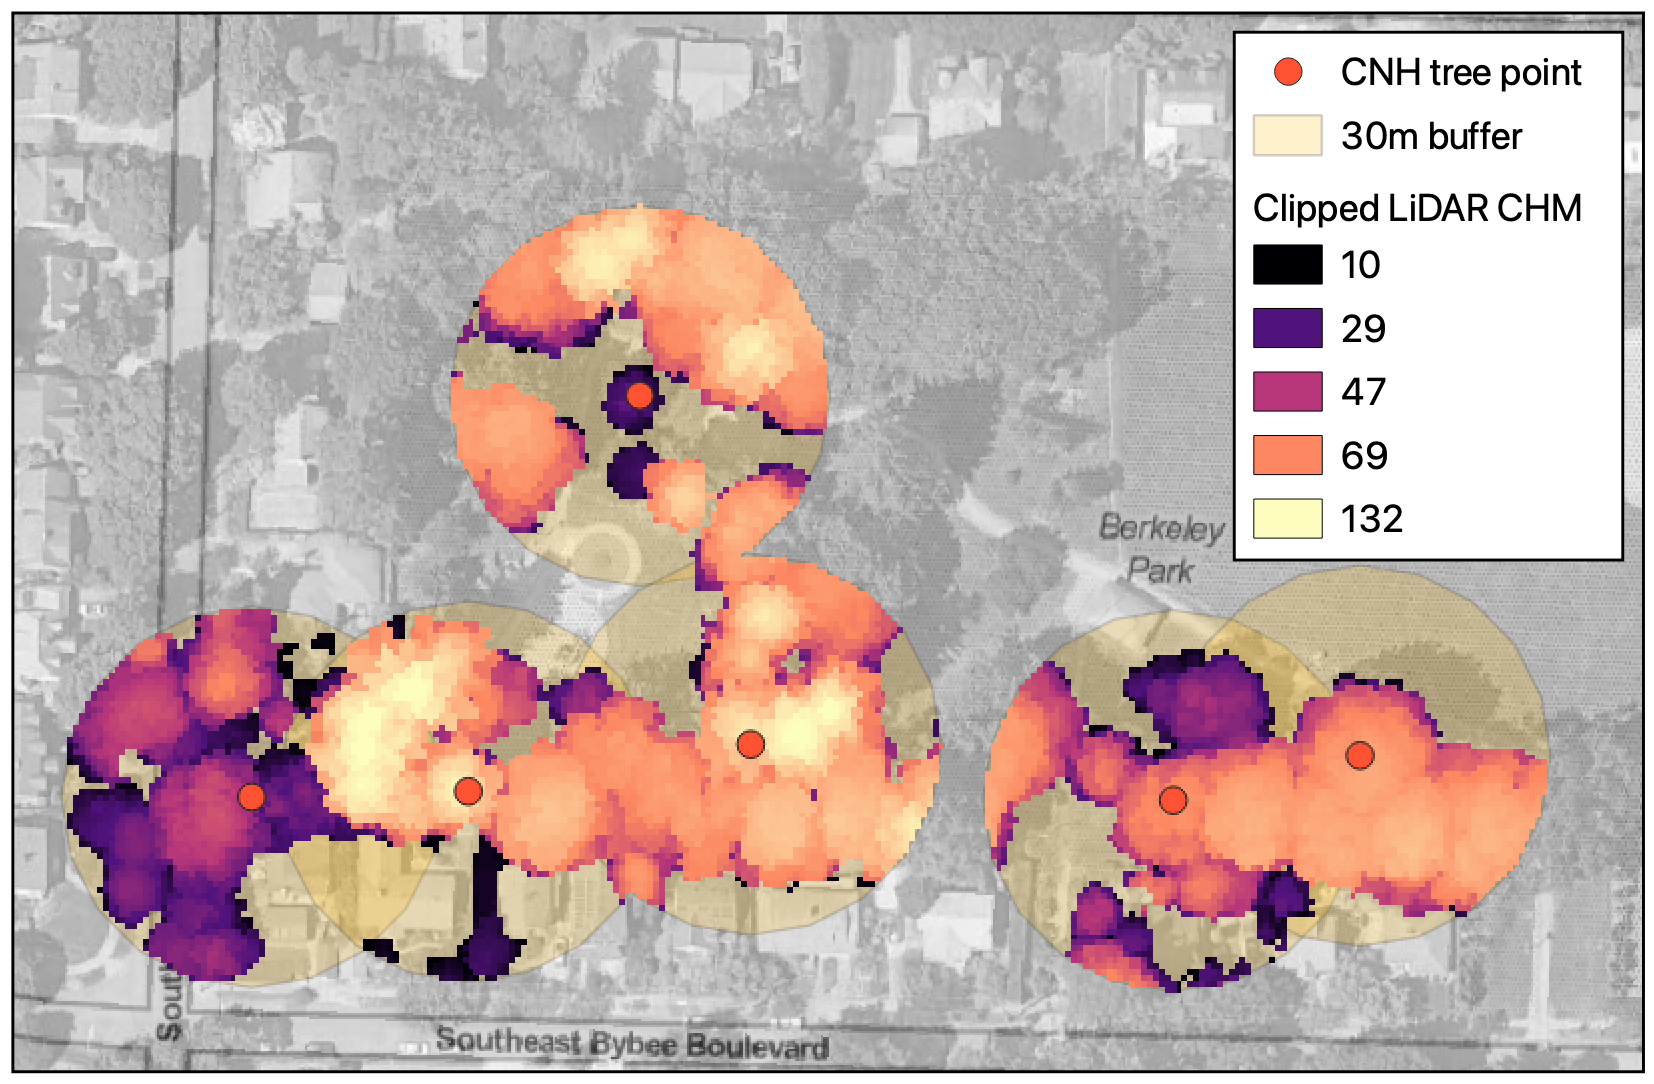
\includegraphics[width=0.8\linewidth,]{figure/lidar_buffer_scale} 

}

\caption{LiDAR data clipped to 30m tree buffer}\label{fig:lidar-buffer}
\end{figure}
\begin{figure}[H]

{\centering 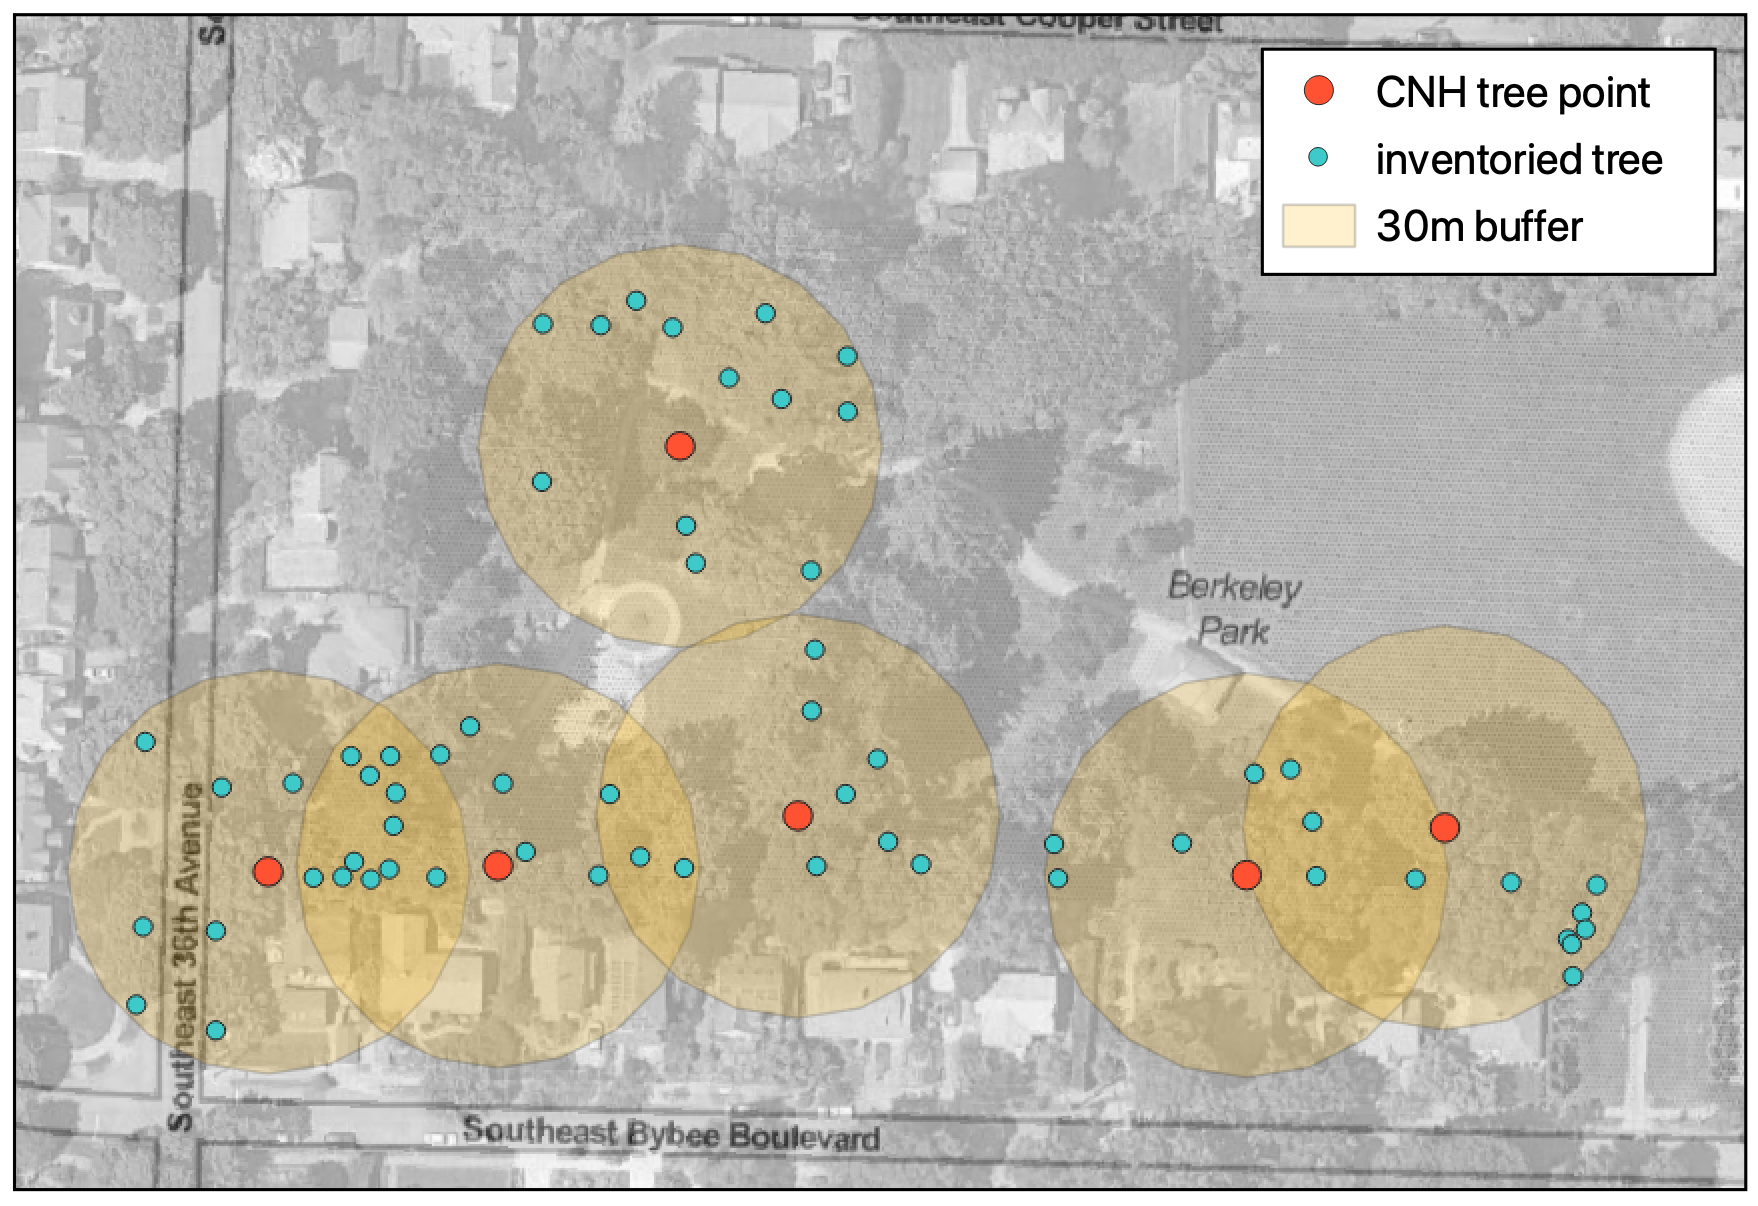
\includegraphics[width=0.8\linewidth,]{figure/buffer_all_points} 

}

\caption{All inventoried trees within the 30m buffer}\label{fig:buffer-points}
\end{figure}
\begin{figure}[H]

{\centering 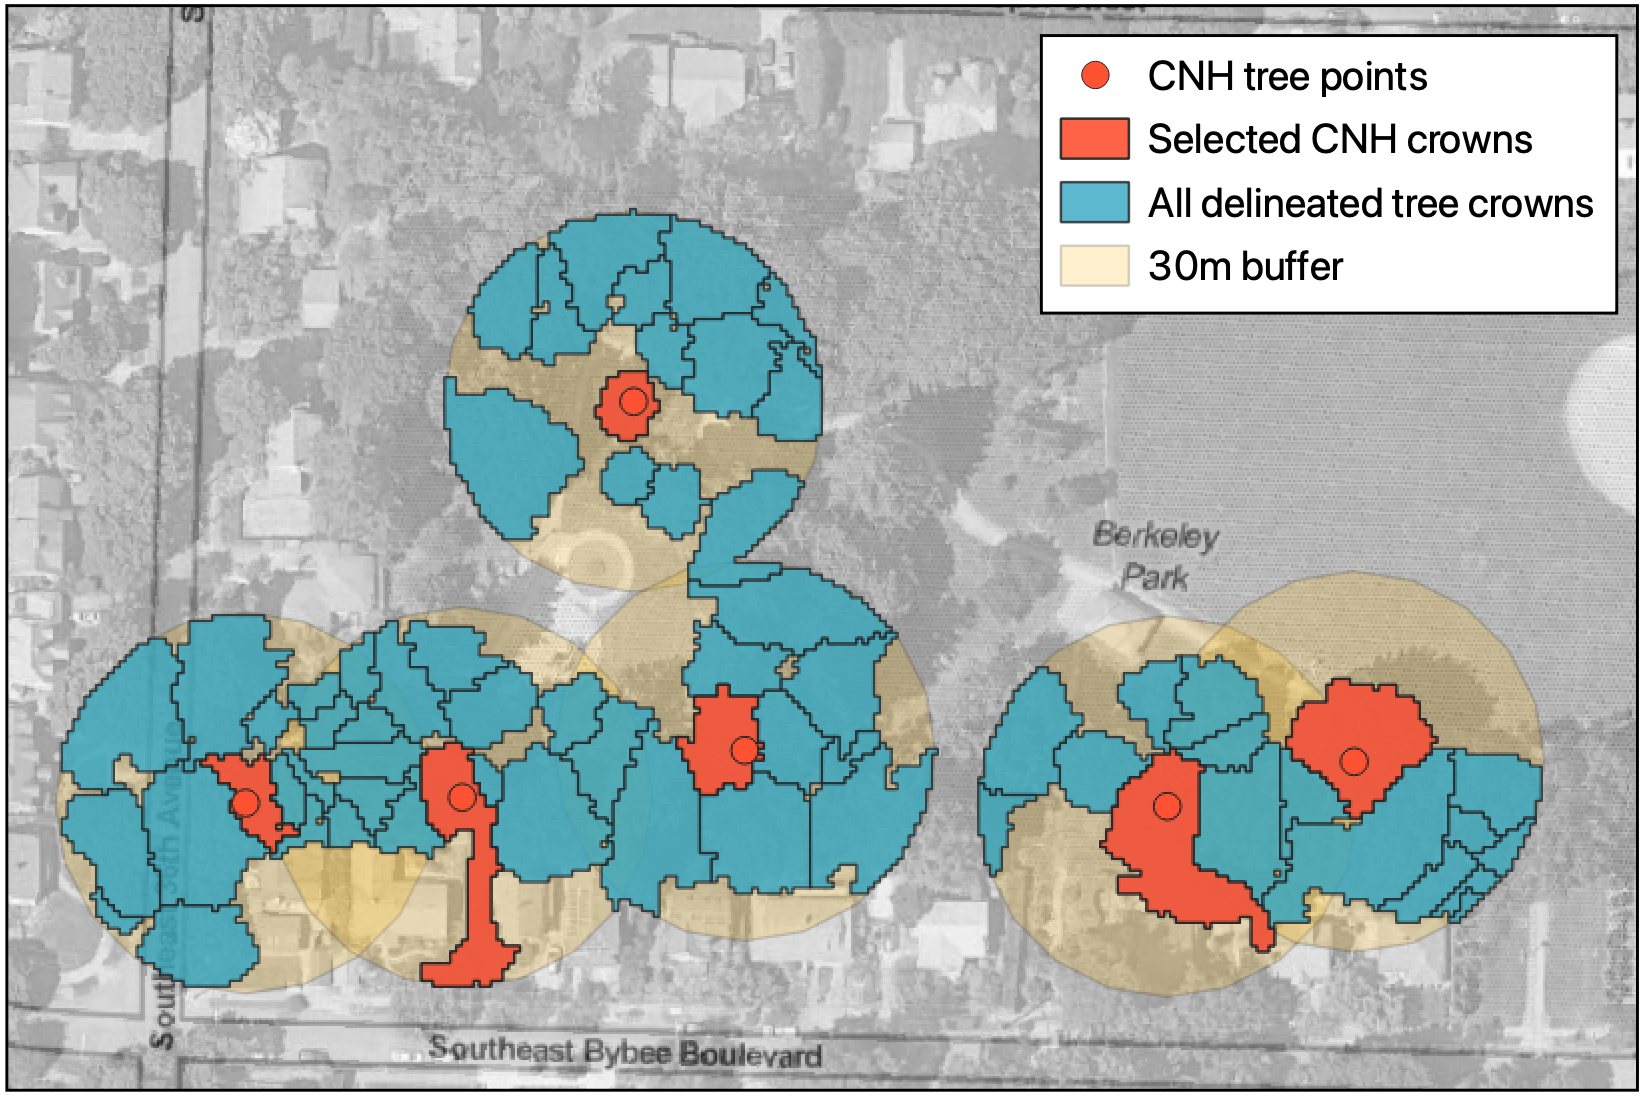
\includegraphics[width=0.8\linewidth,]{figure/selected_lidar} 

}

\caption{LiDAR tree crown delineations with selected CNH crowns}\label{fig:unnamed-chunk-4}
\end{figure}
\begin{figure}[H]

{\centering 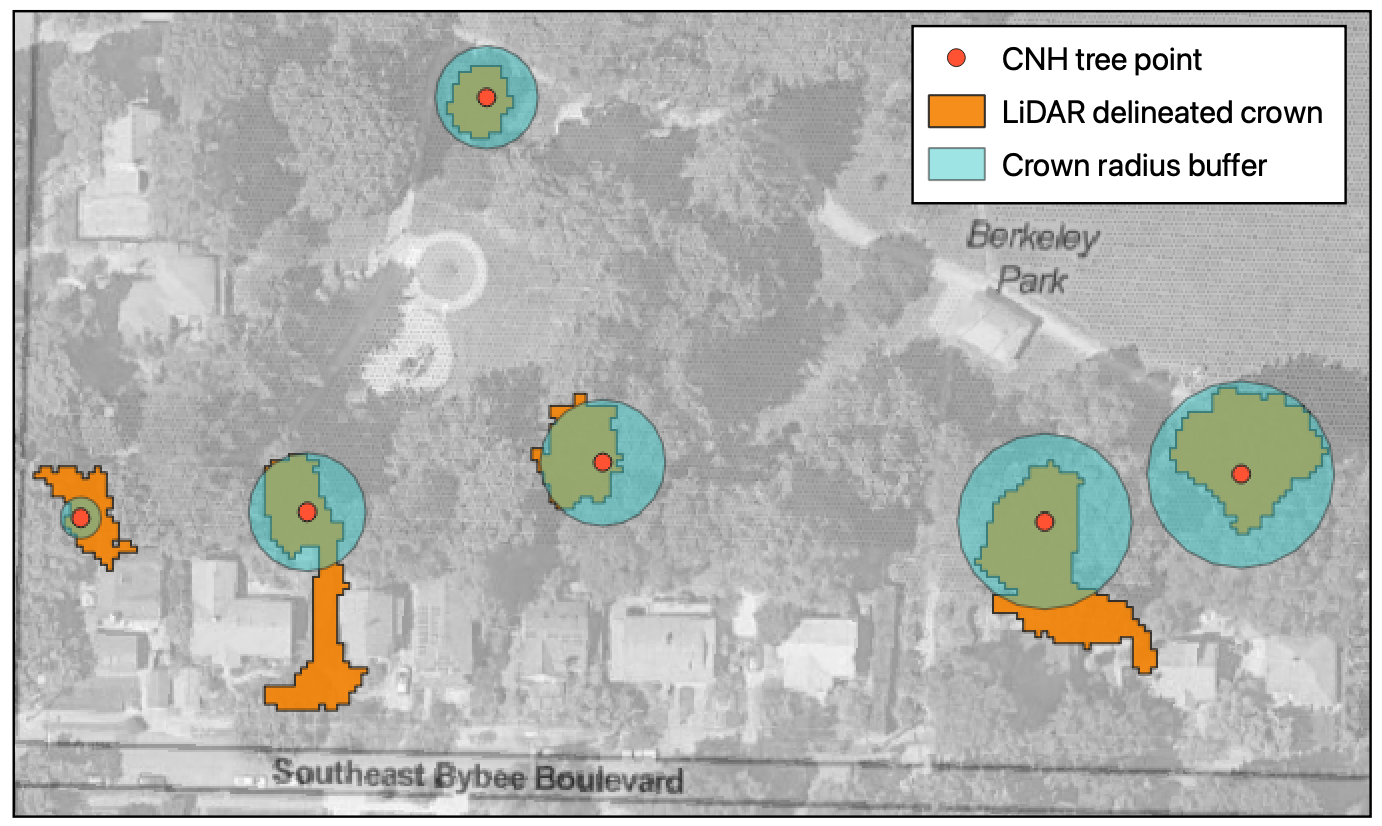
\includegraphics[width=0.9\linewidth,]{figure/layered_outputs} 

}

\caption[Pixel selection method comparison]{Point, Radius, and LiDAR pixel selection methods for Berkeley Park}\label{fig:layered-outputs}
\end{figure}
These three processes were repeated for random samples of 100 park trees
and 100 street trees, stratified for tree species. Due to restrictions
in file size for LiDAR processing, the sampling had to be constrained to
an area of East Portland (Figure \ref{fig:clip-extent}). This extent
was chosen to align with the sampling region of the CNH data, though it
had to be shrunk slightly.
\begin{figure}[H]

{\centering 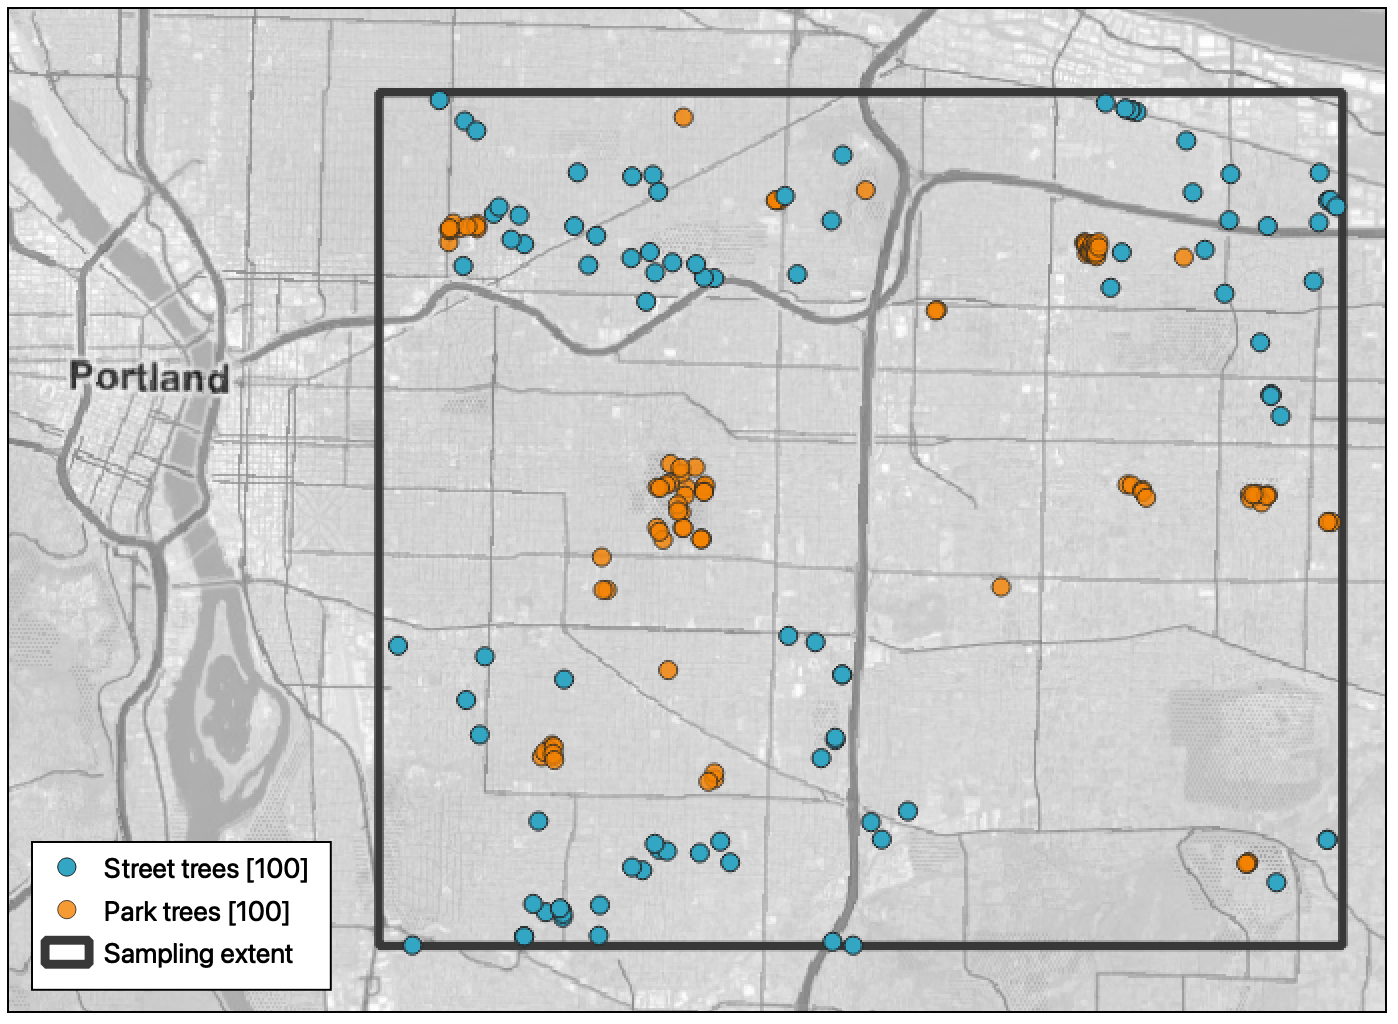
\includegraphics[width=0.8\linewidth,]{figure/extent_and_samples} 

}

\caption{Geographic extent and random sampling}\label{fig:clip-extent}
\end{figure}
\begin{figure}[H]

{\centering 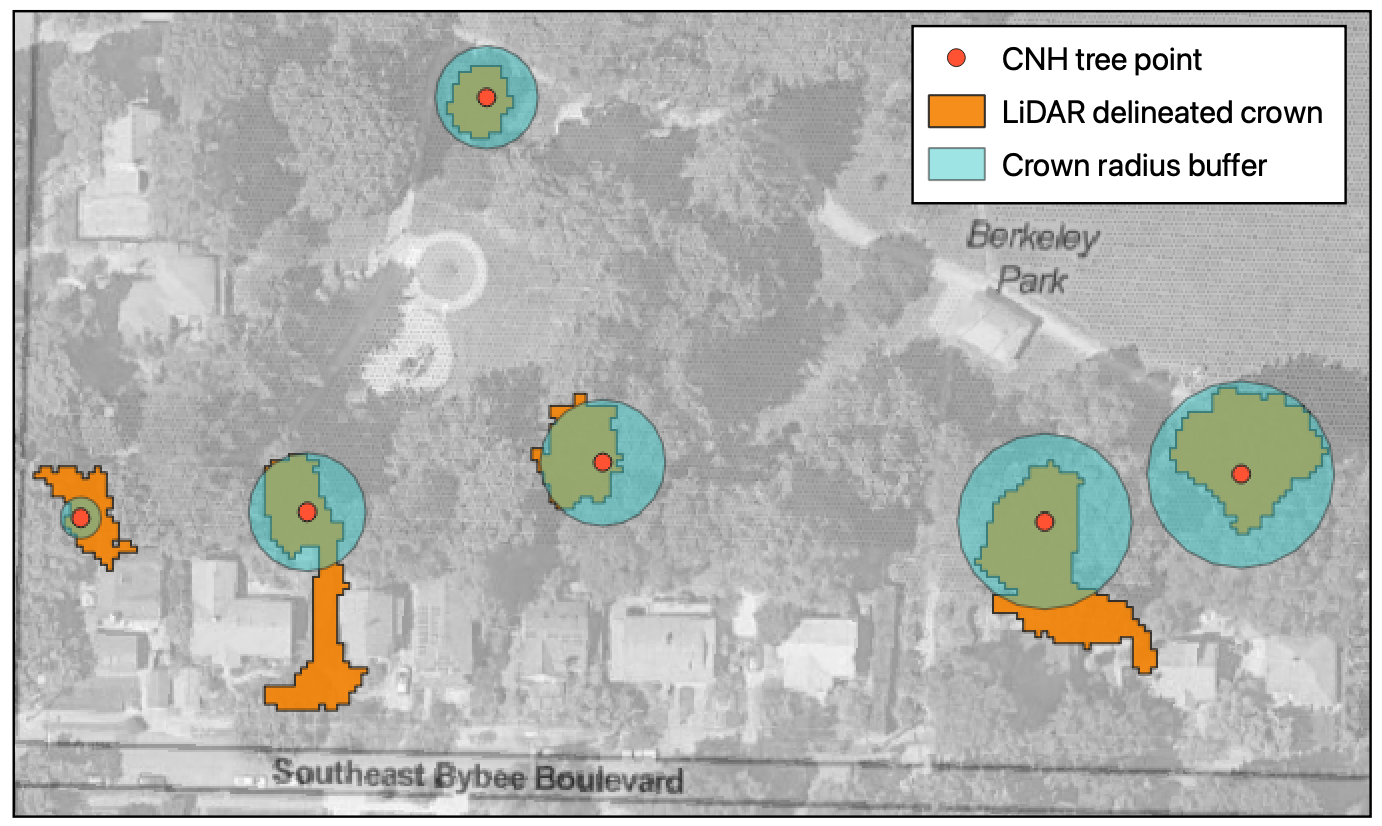
\includegraphics[width=0.8\linewidth,]{figure/layered_outputs} 

}

\caption{LiDAR tree crown delineations with selected CNH crowns}\label{fig:unnamed-chunk-5}
\end{figure}
\hypertarget{modeling-tree-health}{%
\section{Modeling Tree Health}\label{modeling-tree-health}}

To tie all of my smaller pieces of data analysis together, I created a
model to predict tree health categorization from NDVI values. I chose an
ordinal logistic regression, which is used to model and predict the
relationship between an ordinal categorical response variable and one or
more explanatory variables, which can be either categorical or
continuous. An ordinal logistic regression (OLR) is applicable when
there are three or more categories that have a natural and inherent
ordering of levels, but the intervals between these levels are not
necessarily equal. an OLR model is a modified binary logistic regression
model that incorporates the ordinal nature of the dependent variable by
defining the probabilities differently. Instead of solely considering
the probability of an individual event, an OLR considers the
probabilities of that event and all events that are ordered before it
(Shi, n.d.; Venables et al. 2002). The function \texttt{polr()} within the \texttt{MASS} R package is
used to fit a logistic regression model to an ordered factor response
(Ripley 2021).

In order to use this type of model, I tested each model for the
Proportional Odds Assumption which a necessary prerequisite of running
an ordinal logistic regression. I used the Brant Test for ordinal logit
models which is in the \texttt{brant} package (Schlegel et al. 2020; Brant 1990).

For each model, I created a confusion matrix to examine the validity of
the model. A confusion matrix is a calculated cross-tabulation of
observed and predicted classes, which in this case is health
categorization, along with associated statistics. The two main
statistics I use in my data analysis are overall accuracy and an
un-weighted Kappa statistic. ``Accuracy'' \eqref{eq:accuracy} refers to the
sensitivity \eqref{eq:sensitivity} and specificity \eqref{eq:specificity}
of the prediction.
\begin{equation}
  \textrm{Sensitivity}= \frac{\textrm{True positive}}{\textrm{True positive + False negative}}
  \label{eq:sensitivity}
\end{equation}
\begin{equation}
  \textrm{Specificity}= \frac{\textrm{True negative}}{\textrm{True negative + False positive}}
  \label{eq:specificity}
\end{equation}
\begin{equation}
  \textrm{Accuracy}= \frac{\textrm{Sensitivity + Specificity}}{2}
  \label{eq:accuracy}
\end{equation}
Kappa (\(\kappa\)) refers to Cohen's Kappa Statistic which is used to
measure inter and intra-rater reliability for categorical items
\eqref{eq:kappa} (McHugh 2012; Cohen 1960). In this case, the ``raters''
are the measured vs predicted health categorizations.
\begin{equation}
  \kappa = \frac{p_o - p_e}{1 - p_e} = \frac{1 - p_o}{1 - p_e}
  \label{eq:kappa}
\end{equation}
where \(p_o\) is the relative observed agreement between the reference and
prediction, and \(p_e\) is the hypothetical probability of agreement by
chance.

For \(k\) categories, \(N\) observations to categorize and \(n_{ki}\) the
number of times rater \(i\) predicted category \(k\):
\begin{equation}
\mathrm{p_e} = \frac{1}{N^2}\sum{n_{k1}n_{k2}}
\end{equation}
\begin{equation}
  \mathrm{p_e} = \sum_{k}\widehat{p_{k12}} = \sum_{k} \widehat{p_{k1}}\widehat{p_{k2}} = \sum_{k}\frac{n_{k1}}{N}\frac{n_{k2}}{N} =            \frac{1}{N^2}\sum{n_{k1}n_{k2}}
\end{equation}
Where \(\widehat{p_{k12}}\) is the estimated probability that both raters
1 and 2 will classify the same item as category \(k\), while
\(\widehat{p_{k1}}\) is the estimated probabilities that rater 1 will
classify an item as category \(k\). This is based on the assumption that
the rating of the two raters are independent. \(\widehat{p_{k1}}\) is
estimated from the number of items classified as category \(k\) by rater 1
(\(n_{k1}\)) divided by the total number of items for classification
(\(N\)):\(\widehat{p_{k1}}=\frac{n_{k2}}{N}\). These equations and
relationships are the same for rater 2. If the two raters (in this case
the reference and prediction categorizations) are in complete agreement,
then kappa = 1.

For each model, I evaluate the success and ability to predict health
rating in a few different ways. First, I examine the calculated accuracy
and kappa values. A higher kappa value is more important than a higher
accuracy score because kappa takes into account the various sizes of the
categories and the probability of the prediction occurring by chance,
whereas accuracy does not. Additionally, I look at the false positives
(a \textbf{poor} tree getting rated \textbf{good}) and false negatives (a \textbf{good}
tree being rated \textbf{poor}). Both of these values should be as low as
possible, but in this case reducing the number of false positives is
most important because if a tree in \textbf{poor} health was rated as
\textbf{good}, it may not be included in further health analysis and will be
missed when examining the spatial distribution of tree health.

\hypertarget{results}{%
\chapter{Results}\label{results}}

\hypertarget{canopy-model-results}{%
\section{Canopy Width and Tree Height Model}\label{canopy-model-results}}

I used a second order polynomial regression to predict both tree height
and crown width from tree DBH. The tree height predictions were used to
filter out trees below 25 feet in height, and the crown width
predictions were used in the radius method of pixel selection for NDVI
analysis. There are numerous expected differences between the species
due to functional tree type. For example, the average DBH for ACMA and
PSME are relatively close, but the average height for a PSME individual
is nearly twice as tall as an ACMA (Table \ref{tab:tree-stats-table}).
Because of this, DBH would have a very different effect on the outcome
of both models depending on the species of the tree. I included species
as an interaction term in the model to account for these expected
differences between species, meaning that both DBH and species were used
to predict crown width and tree height. I tested a linear model as well
as second and third order polynomial models for both predictive models
(Figures \ref{fig:test-height-model}, \ref{fig:test-width-model}). A
second order polynomial was chosen for the predictive models because it
not only encapsulated the relationship between DBH and tree height as
well as DBH and canopy width, but it also was the most accurate when
modeling the individual species. When I modeled each species
individually for both tree height and canopy width, I got the same
results as if I created one model and included species as an interaction
term.
\begin{table}[H]

\caption[Physiological Tree Measurements]{\label{tab:tree-stats-table}Average physiological measurements for selected species in the Park Trees database.}
\centering
\begin{tabular}[t]{lrrr}
\toprule
Species & Avg. DBH & Avg. Tree Height & Avg. Crown Width\\
\midrule
ACMA & 29.28 & 69.49 & 49.39\\
ACPL & 20.34 & 49.77 & 44.80\\
PSME & 29.57 & 112.14 & 39.47\\
THPL & 18.11 & 50.14 & 24.14\\
\bottomrule
\end{tabular}
\end{table}
The tree height model has an adjusted R-squared value of 0.7834, and a
P-value of \textless{} 2.2e-16 (Figure \ref{fig:height-model}, Appendix
equations \eqref{eq:a1}, \eqref{eq:a3}, \eqref{eq:a5}, \eqref{eq:a7}). This
model was most effective for ACMA and PSME, but was not statistically
significant for ACPL or THPL. This is likely due to the similar average
DBH and tree height values between ACMA and PSME. While the average DBH
values for ACMA and PSME are very similar, the average height values are
extremely different, with the average PSME individual standing twice as
tall as the average ACMA individual (Table \ref{tab:tree-stats-table}).
An issue with the second degree model is the decrease in predicted tree
height. This decrease is not seen in the park tree model, but the street
tree height predictions for all species show a visible decrease after
the inflection point of the model. Given that the tree height
predictions were only used for filtering out trees below 25 feet in
height, an extremely precise model was not necessary for the purposes of
this thesis.

The crown width model has an adjusted R-squared value of 0.7269, and a
P-value of \textless{} 2.2e-16 (Figure \ref{fig:width-model-g}, Appendix
equations \eqref{eq:a2}, \eqref{eq:a4}, \eqref{eq:a6}, \eqref{eq:a8}). The
coefficients for the canopy width model had statistically significant
p-values for all species. There is consistent variation in the average
crown width measurements between all species (Table
\ref{tab:tree-stats-table}). With the visualization of the street tree
canopy width predictions, the only extreme decrease after the model
inflection point is seen in the ACPL predictions. The canopy width model
played a larger role in this thesis than the tree height model because
it was essential for the radius method of pixel selection for all street
trees.
\begin{figure}[H]

{\centering 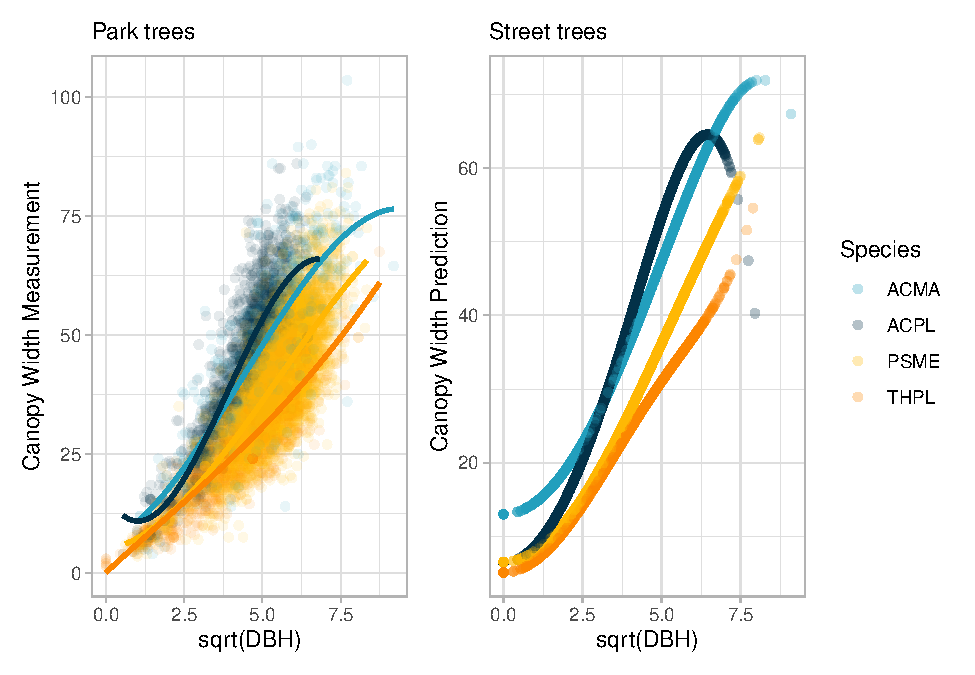
\includegraphics[width=0.8\linewidth,]{thesis_files/figure-latex/width-model-g-1} 

}

\caption[Crown width predictive model]{Second order polynomial model for predicting tree crown width based on measured DBH and species, with predictions for street trees. (R-squared = 0.7269,  P < 2.2e-16)}\label{fig:width-model-g}
\end{figure}
\hypertarget{health-rating-vs.-tree-type-and-tree-species}{%
\section{Health Rating vs.~Tree Type and Tree Species}\label{health-rating-vs.-tree-type-and-tree-species}}

For all trees collected as part of the CNH field work, I examined the
potential existing relationships between measured health rating and tree
functional type, as well as between health rating and tree species. A
Chi-Square Test of Independence was performed to assess the relationship
between health rating and functional tree type. There was a significant
relationship between the two variables (\(X^2\)(2, N=112) = 10.184, p =
0.00615). Within functional tree type, both conifers and broadleaf trees
were most likely to be rated as \textbf{fair}, but within health category a
\textbf{good} or a \textbf{poor} tree were most likely a broadleaf tree, and a
\textbf{fair} tree was most likely a conifer (Tables
\ref{tab:table-freq-test-1}, \ref{tab:table-freq-test-2}). A
Chi-Square Test of Independence was performed to assess the relationship
between health rating and tree species. There was a significant
relationship between the two variables (\(X^2\)(6, N=112) = 22.368, p =
0.00104). Within tree species, ACMA, PSME, and THPL were all most likely
to be rated as \textbf{fair}, but ACPL was most likely to be rated as
\textbf{good}. Within health category, a \textbf{poor} tree was most likely an
ACMA individual, a \textbf{fair} tree was equally likely to be a PSME or THPL
individual, and a \textbf{good} tree was most likely an ACPL individual
(Tables \ref{tab:table-freq-test-3}, \ref{tab:table-freq-test-4}).
\begin{longtable}[t]{lrr}
\caption[Frequency table of functional tree type and health rating for CNH trees]{\label{tab:table-freq-test-1}Frequency table of functional tree type and health rating for CNH trees. There is a statistically significant relationship between the two variables ($X^2$(2, N=112) = 10.184, p = 0.00615)}\\
\toprule
  & broadleaf & conifer\\
\midrule
poor & 9 & 6\\
fair & 28 & 40\\
good & 22 & 7\\
\bottomrule
\end{longtable}
\begin{longtable}[t]{lrr}
\caption[Probability table of functional tree type and health rating for CNH trees]{\label{tab:table-freq-test-2}Probability table of functional tree type and health rating for CNH trees. }\\
\toprule
  & broadleaf & conifer\\
\midrule
poor & 0.0803571 & 0.0535714\\
fair & 0.2500000 & 0.3571429\\
good & 0.1964286 & 0.0625000\\
\bottomrule
\end{longtable}
\begin{longtable}[t]{lrrrr}
\caption[Frequency table of functional tree type and health rating for CNH trees]{\label{tab:table-freq-test-3}Frequency table of functional tree type and health rating for CNH trees. There is a statistically significant relationship between the two variables ($X^2$(2, N=112) = 10.184, p = 0.00615)}\\
\toprule
  & ACMA & ACPL & PSME & THPL\\
\midrule
poor & 7 & 2 & 1 & 5\\
fair & 16 & 12 & 20 & 20\\
good & 6 & 16 & 4 & 3\\
\bottomrule
\end{longtable}
\begin{longtable}[t]{lrrrr}
\caption[Probability table of functional tree type and health rating for CNH trees]{\label{tab:table-freq-test-4}Probability table of functional tree type and health rating for CNH trees.}\\
\toprule
  & ACMA & ACPL & PSME & THPL\\
\midrule
poor & 0.0625000 & 0.0178571 & 0.0089286 & 0.0446429\\
fair & 0.1428571 & 0.1071429 & 0.1785714 & 0.1785714\\
good & 0.0535714 & 0.1428571 & 0.0357143 & 0.0267857\\
\bottomrule
\end{longtable}
\hypertarget{health-rating-vs.-ndvi-point-method-obtained-data}{%
\section{Health Rating vs.~NDVI: Point Method Obtained Data}\label{health-rating-vs.-ndvi-point-method-obtained-data}}

With the selection of CNH trees and 2021 NDVI data, a statistical
analysis of the point value method shows that there is a statistically
significant difference in NDVI values between health categorizations of
\textbf{fair} and \textbf{good} (ANOVA, \(F_{2, 109} = 3.892\), \(P = 0.023\),
TukeyHSD). There is a general positive correlation between NDVI and
health category, specifically \textbf{fair} and \textbf{good}. The relationship
between health and NDVI is more apparent in the two maple species, but
still holds in the \textbf{fair} and \textbf{good} categories in the two
coniferous species (Figure \ref{fig:point-species}). While the
difference between NDVI values and health ratings is statistically
significant for the point data as a whole, this is not true for all
species. The difference in NDVI between \textbf{fair} and \textbf{good} rated
trees is only statistically significant for THPL, meaning that this
statistically significant relationship in the point method data is
entirely driven by the THPL measurements (ANOVA: \(F_{2, 25} = 3.834\),
\(P = 0.0353\); TukeyHSD: \textbf{good}-\textbf{fair} \(P = 0.031\)). There is no
statistical significance when split by functional tree type.





\begin{figure}[H]

{\centering 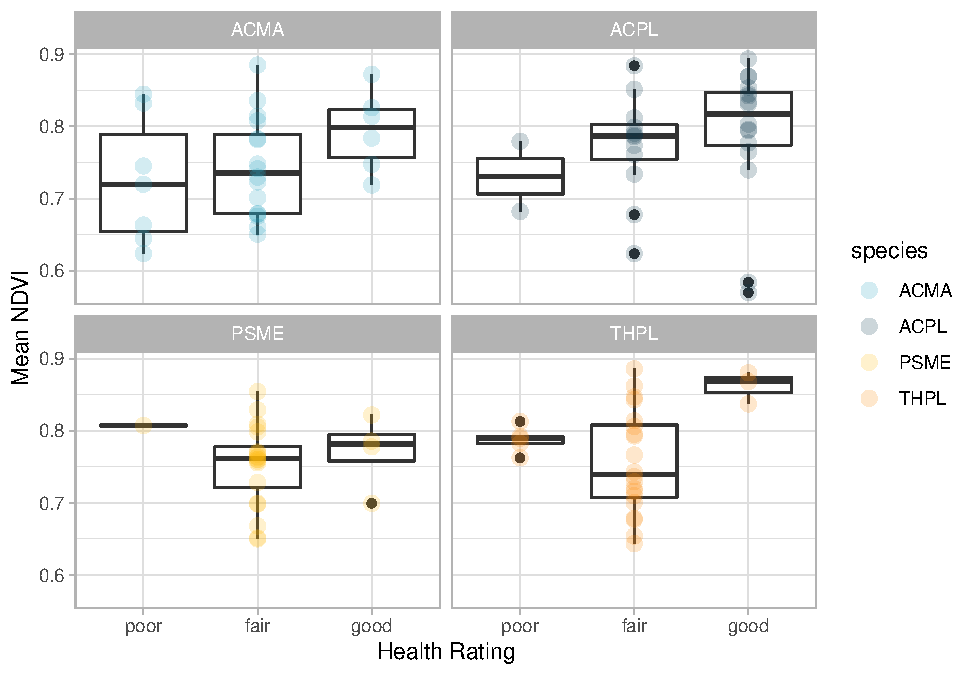
\includegraphics[width=1\linewidth,]{thesis_files/figure-latex/point-species-1} 

}

\caption[Point Method NDVI and Health Rating, by Species]{NDVI extracted for CNH trees using the point method
compared to CNH tree health categorization. There is a statistically
significant difference between \textbf{fair} and \textbf{good} (ANOVA,
\(F_{2, 109} = 3.892\), \(P = 0.023\), TukeyHSD)}\label{fig:point-species}
\end{figure}
\hypertarget{health-rating-vs.-ndvi-radius-method-obtained-data}{%
\section{Health Rating vs.~NDVI: Radius Method Obtained Data}\label{health-rating-vs.-ndvi-radius-method-obtained-data}}

With the radius method of pixel selection and crown delineation, there
is a statistically significant difference in the mean NDVI values for
health categories (ANOVA, \(F_{2,109}=4.923\), \(P = 0.0089\); TukeyHSD:
\textbf{good-poor} \(P = 0.033\), \textbf{good-fair} \(P = 0.014\)). Similar to the
point method, there is a larger difference in average NDVI between the
\textbf{fair} vs \textbf{good} categories than \textbf{poor} vs \textbf{fair}, which is
statistically significant in the radius method results (Figure
\ref{fig:radius-species}). When the statistical analysis is split by
tree species, there is no statistical significance. When split by
functional tree type, there is a statistcally significant difference in
the NDVI values between \textbf{good} and \textbf{poor} health ratings for
broadleaf trees (ANOVA, \(F_{2,56}=3.976\), \(P = 0.0243\), TukeyHSD).
\begin{figure}[H]

{\centering 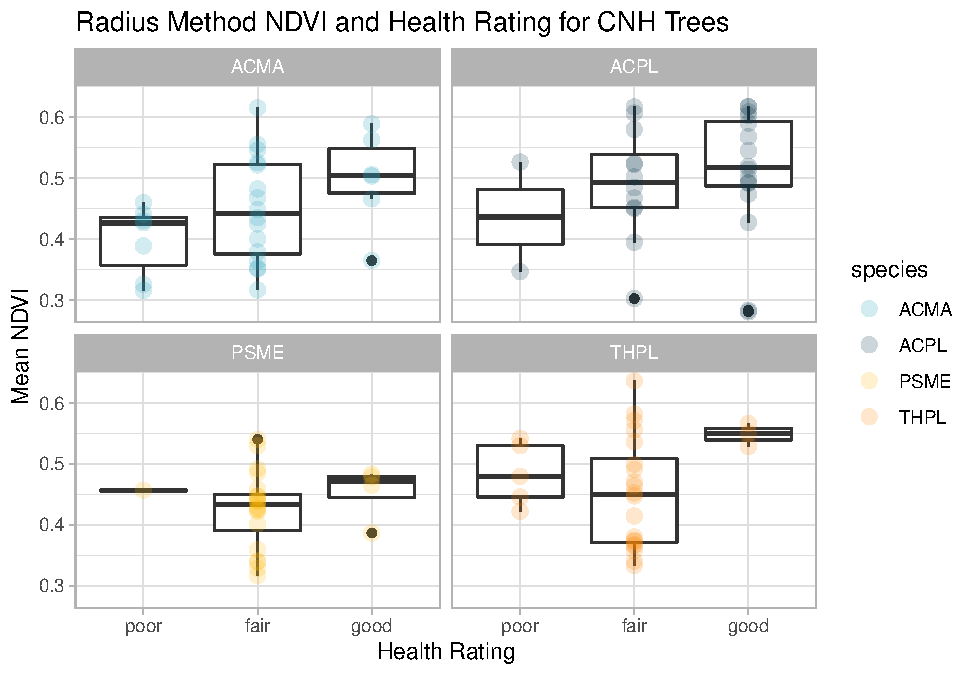
\includegraphics[width=1\linewidth,]{thesis_files/figure-latex/radius-species-1} 

}

\caption[Radius method mean NDVI and health condition by species]{Boxplot of average NDVI from radius method and health condition, by species. The relationship between NDVI and health category is strongest in the maples, but still somewhat aparent in the conifers. (ANOVA, $F_{2,109}=4.923$, $P = 0.0089$; TukeyHSD: good-poor $P = 0.033$, good-fair $P = 0.014$)}\label{fig:radius-species}
\end{figure}
\hypertarget{health-rating-vs.-ndvi-lidar-method-obtained-data}{%
\section{Health Rating vs.~NDVI: LiDAR Method Obtained Data}\label{health-rating-vs.-ndvi-lidar-method-obtained-data}}

There is a statistically significant difference in NDVI between health
categories for the LiDAR method, specifically between \textbf{good} and
\textbf{fair} (ANOVA, \(F_{2,101} = 5.405\), \(P = 0.00589\), TukeyHSD). The same
relationship between NDVI and health condition for the maples that was
seen in the point and radius method is seen here (Figure
\ref{fig:lidar-species}). Again, when split by species, there is no
statistical significance. However, when split by functional tree type
there is a statistically significant difference between the average NDVI
values for \textbf{good} and \textbf{poor} health categories for broadleaf trees
(ANOVA, \(F_{2,51} = 3.498\), \(P = 0.0377\), TukeyHSD).







\begin{figure}[H]

{\centering 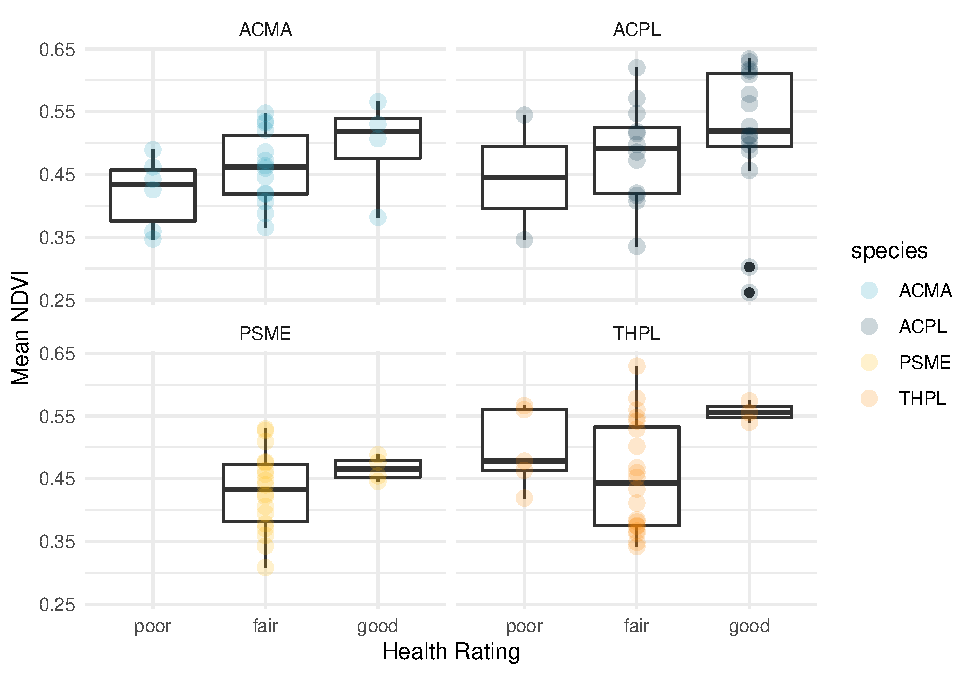
\includegraphics[width=1\linewidth,]{thesis_files/figure-latex/lidar-species-1} 

}

\caption[NDVI and health condition for LiDAR method]{Boxplot of average NDVI from LiDAR method and health
condition for each species. Due to the nature of the LiDAR delineation
algorithm, no crown was detected for the PSME individual with a \textbf{poor}
health rating. The difference between \textbf{good} and \textbf{fair} average
NDVIs is statistically significant (ANOVA, \(F_{2,101} = 5.405\),
\(P = 0.00589\), TukeyHSD)}\label{fig:lidar-species}
\end{figure}
Another aspect of the LiDAR delineation method is the potential for data
loss. Five ACMA and three PSME individuals were lost in the LiDAR crown
delineation process. If this was with a very large sample size the data
loss would likely not be detrimental but especially with a sample size
such as mine, a loss of eight trees is a loss of 5\% of the total data,
17\% loss for ACMA, and 12\% loss for THPL.

\hypertarget{method-comparison}{%
\section{Method Comparison}\label{method-comparison}}

There is no statistically significant difference in NDVI values for the
three different pixel selection methods, which were standardized to
z-scores for NDVI (ANOVA, \(F_{2, 325}=0\), \(P = 1\)). For each method,
Z-scores were calculated for the NDVI values. The mean Z-score for point
method NDVI for trees rated \textbf{poor} is above zero meaning that the raw
NDVI value for a \textbf{poor} rated tree is higher than the mean average
NDVI value for point method trees. For the radius and LiDAR data, the
average z-score for \textbf{poor} rated trees is below the mean average NDVI
value for each method. Interestingly, the mean z-score for \textbf{poor}
LiDAR trees is higher than for \textbf{fair} trees (Figure
\ref{fig:methods-all-species}).

When the species are clumped with raw NDVI measurements, the three
methods show very similar patterns, though the NDVI values are higher
for the point method than either of the other two methods (Figure
\ref{fig:methods-species}). When all three methods are compared along
with species, we can see that the general trend of health rating and
NDVI is consistent within each species. The pattern between health
rating and NDVI is also very similar between trees of the same
functional type (Figure \ref{fig:methods-species}). Because of these
similarities in health rating and NDVI values for trees belonging to the
same functional type, I included additional testing examining the
difference in species specificity addition versus functional type
separation.
\begin{figure}[H]

{\centering 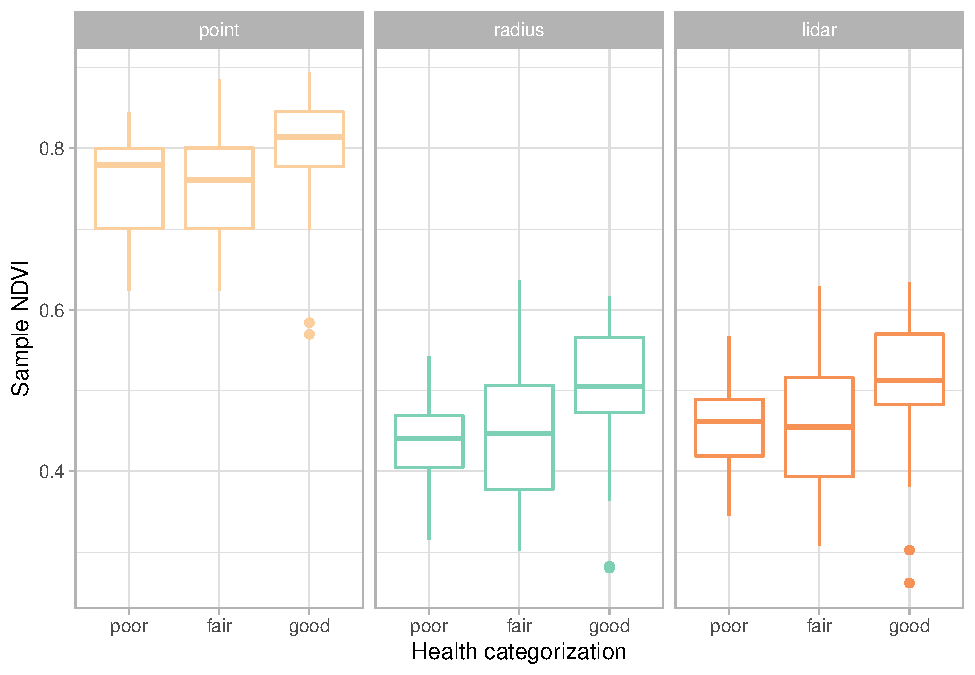
\includegraphics[width=0.8\linewidth,]{thesis_files/figure-latex/methods-all-species-1} 

}

\caption[Z-score of NDVI and health rating comparison across methods]{Z-score of NDVI values from all three pixel selection methods with CNH health rating. There is no statistically significant difference in NDVI trends between pixel selection methods. (ANOVA, $F_{2, 325}=0$, $P = 1$)}\label{fig:methods-all-species}
\end{figure}
\begin{figure}[H]

{\centering 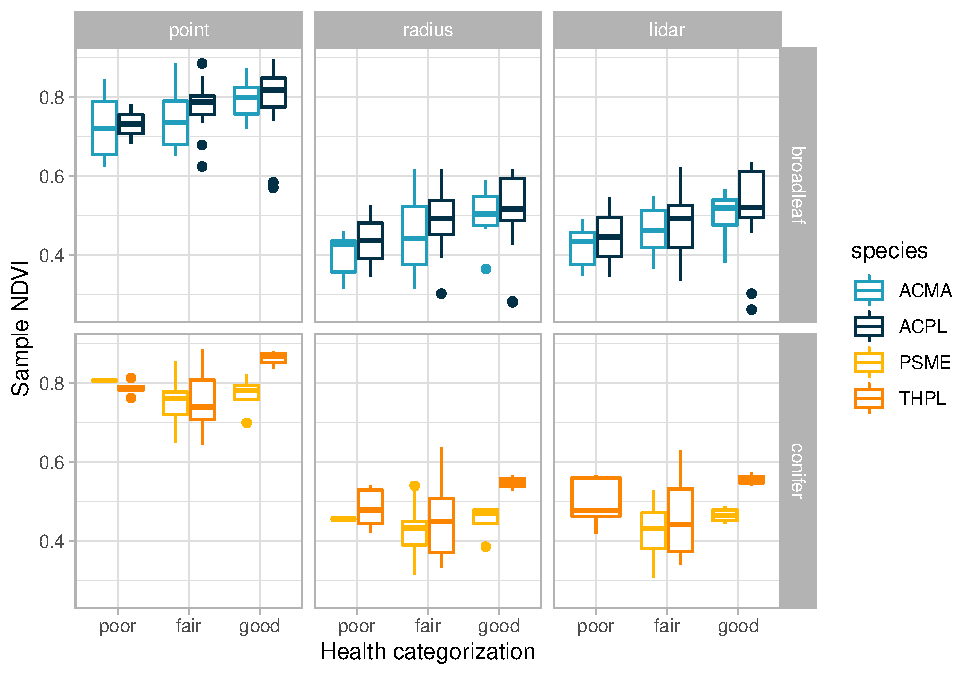
\includegraphics[width=0.9\linewidth,]{thesis_files/figure-latex/methods-species-1} 

}

\caption[Average NDVI comparison between species and methods.]{Average NDVI for each health category, split by functional tree type and pixel selection method. The general trends remain the same for each individual species, but varies between functional type. The same trends can be seen for trees of the same functional type (broadleaf vs conifer).}\label{fig:methods-species}
\end{figure}
Another important factor to consider when comparing the three pixel
selection methods is the amount of pixels used in the NDVI analysis. For
the point method, each NDVI value is based off one singular point. For
both LiDAR and Radius methods, the NDVI used in prediction is an average
of all NDVI values captured within the pixel selection method, but the
number of pixels used varies between methods and species (Figure
\ref{fig:ndvi-counts-graph}).
\begin{figure}[H]

{\centering 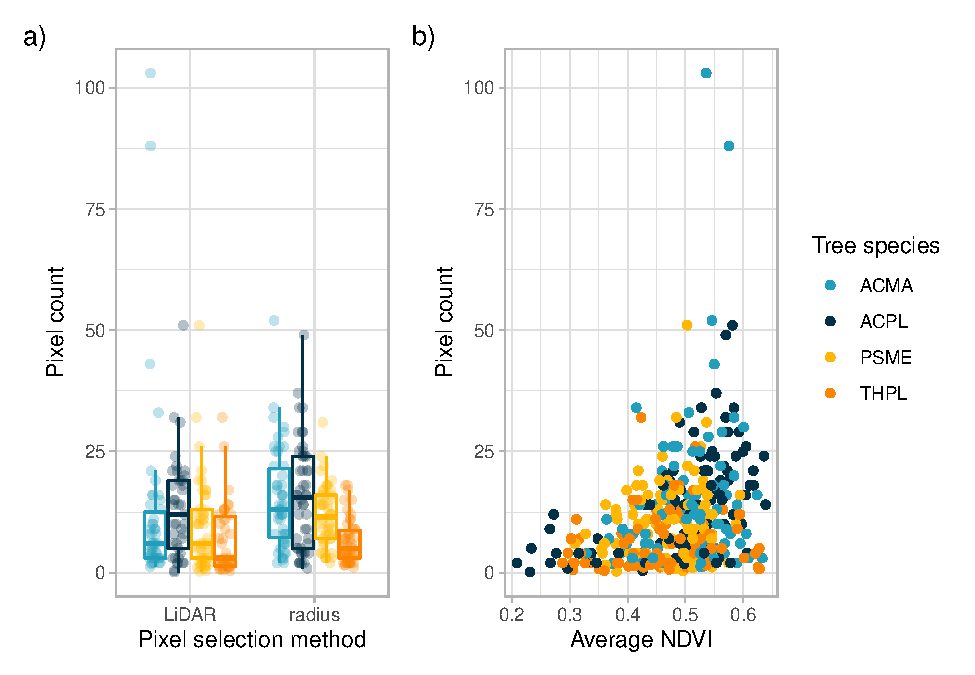
\includegraphics[width=0.9\linewidth,]{thesis_files/figure-latex/ndvi-counts-graph-1} 

}

\caption[Pixel counts for NDVI calculation, by method, and for sample NDVI.]{Comparison of pixel counts used in NDVI calculations. (a) Boxplot of pixel counts used for each species in the LiDAR and radius methods. For both methods, the maples had more outliers than the conifers, and THPL had the lowest average number of pixels used. (b) Pixel count and average NDVI per tree.}\label{fig:ndvi-counts-graph}
\end{figure}
\hypertarget{predictive-model}{%
\section{Predictive Model}\label{predictive-model}}

I used ordinal logistic regression models with the goal of predicting
tree health rating from NDVI. In order to determine the impact of
differentiating by species in predictive models, I ran three different
models for each point selection method, moving from least to most
specific: a model that only uses NDVI to predict health rating, a model
that includes functional tree type as an interaction term, and a third
model that includes species as an interaction term (Table
\ref{tab:model-table}).

Due to the limited sample size of the data I am working with, the
following models are trained and tested on the same data, which is the
CNH tree data collected summer 2021. I chose to do this because of the
limited sample size of CNH trees, and the uneven size of the health
category ratings. Because of this, it is important to note that the
model tests are an idealized version of a true model. However, it is
important to note that they are idealized version of how model testing
and training would work in reality.

With the point method data, the first model using only NDVI as a
predictor (health rating \textasciitilde{} point NDVI) led to all tree points being
rated as \textbf{fair} (Figure \ref{fig:point-model-split}a). For the
continuous variable of NDVI, the coefficient value of 7.041 can be
interpreted as that with one unit increase in NDVI, the log of odds of
having a \textbf{good} health rating increase by 7.041. With the t-value of
2.479, this is statistically significant at the .05 level. The intercept
for \textbf{poor} vs \textbf{fair} shows that the log of odds of a tree being
rated as \textbf{poor} versus \textbf{fair} or \textbf{good} is not statistically
significant, but the log odds of a tree being rated \textbf{poor} or \textbf{fair}
versus \textbf{good} are statistically significant.

The model using tree type as an additional predictor (health rating \textasciitilde{}
point NDVI * tree type) had an increase in predictions of \textbf{good}
health trees, and increased kappa from 0\% to 15\% (Figure
\ref{fig:point-model-split}b). The overall accuracy only increased by
2\%, but kappa is more informative in terms of model validity than the
accuracy score. With this model, one unit increase in NDVI will lead to
an increase in the log odds of having a \textbf{good} rating by 10.2 (t-value
= 2.685). The impact of a tree being classified as a conifer, versus a
broadleaf tree, were not statistically significant at the 0.05 level.
Again, the intercept for \textbf{poor} vs \textbf{fair} is not statistically
significant, but the log odds of a tree being rated \textbf{poor} or \textbf{fair}
versus \textbf{good} are statistically significant.

Using tree species instead of tree type in the model (health rating \textasciitilde{}
point NDVI * species) further improved the kappa of the model. The
number of \textbf{good} trees that were correctly predicted increased from 7
to 13, but additionally the number of \textbf{fair} trees that were correctly
predicted dropped from 64 to 59, with the new predictions as \textbf{good}
(Figure \ref{fig:point-model-split}c). None of the models that used the
point method obtained data were able to correctly predict any trees with
\textbf{poor} health categorization, and in models b and c, each had one
\textbf{poor} tree that was incorrectly predicted as \textbf{good}.
\begin{figure}[H]

{\centering 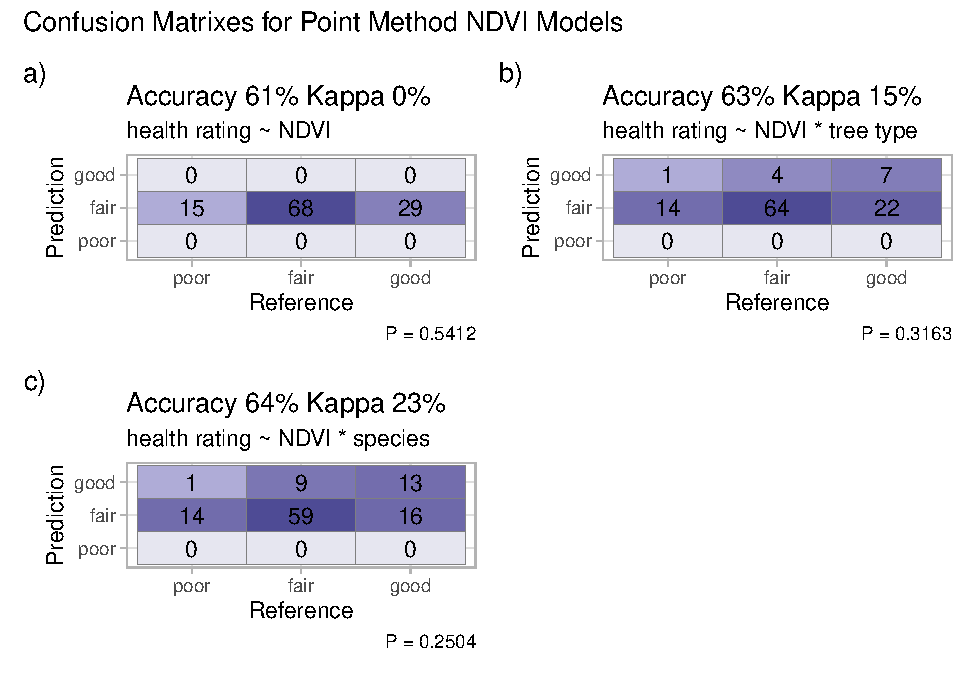
\includegraphics[width=0.9\linewidth,]{thesis_files/figure-latex/point-model-split-1} 

}

\caption[Confusion matrixes for Point method predictive models]{Confusion Matrix results for three predictive models, using point method obtained NDVI data to predict three health rating. (a) Model only using NDVI to predict health rating. (b) Model using both NDVI and functional tree type (broadleaf vs confier) to predict health rating. (c) Model using NDVI and tree species to predict health rating.}\label{fig:point-model-split}
\end{figure}
Using just NDVI as a predictor in the model (health rating \textasciitilde{} radius
NDVI) still performs the worst of the three models, with 96\% of the
sampled trees being predicted as \textbf{fair} (Figure
\ref{fig:radius-model-split}a). Similar to the point method with no
interaction term (health rating \textasciitilde{} point NDVI), the \textbf{fair} vs \textbf{good}
intercept is the only one that is statistically significant. However,
this model has a t value of 3.68, meaning this model performs better
than the point method model with the same formula. When using tree type
as predictor variables (health rating \textasciitilde{} radius NDVI * tree type),
there was an increase in the number of trees being rated as in \textbf{good}
health of 9 trees in total, but only 6 of those were additional correct
predictions (Figure \ref{fig:radius-model-split}b). Again, the
intercept of \textbf{fair} vs \textbf{good} is statistically significant, meaning
that the log of odds of a tree in this model being rated \textbf{poor} or
\textbf{fair} versus \textbf{good}. The main takeaway from the radius method
models is that with the inclusion of species as an interaction term with
the radius data (health rating \textasciitilde{} radius NDVI * species), we see our
first predictions of the \textbf{poor} category. There is no increase in
statistical significance of the log odds between the previous model and
this one. The radius method does involve more pixels than the point
method, and with the range in NDVI values being lower than that of the
point method it makes sense that there is an increase in \textbf{poor} rated
trees. However, out of the 15 reference trees with health ratings of
\textbf{poor}, only one was correctly predicted as such (Figure
\ref{fig:radius-model-split}c).
\begin{figure}[H]

{\centering 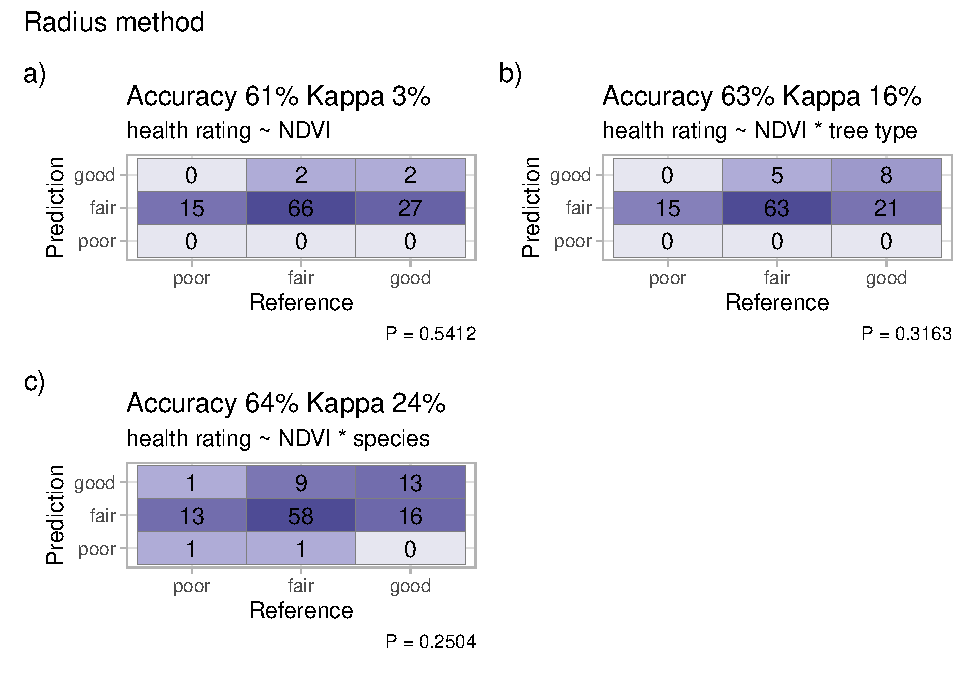
\includegraphics[width=0.9\linewidth,]{thesis_files/figure-latex/radius-model-split-1} 

}

\caption[Confusion matrixes for Radius method predictive models]{Confusion matrixes for each species predictions with radius method data. (a) Model using only NDVI to predict health rating. (b) Model with the addition of functional tree type as a predictor. (c) Model using tree species as a variable when predicting tree health rating.}\label{fig:radius-model-split}
\end{figure}
The LiDAR data was the most effective at predicting tree health across
all three pixel selection methods. With the first model using only NDVI
to predict health rating (health rating \textasciitilde{} LiDAR NDVI), more trees were
correctly predicted as \textbf{good} than the same model with the other two
methods (Figure \ref{fig:lidar-model-split}a). With the addition of
tree type as a predictor variable (health rating \textasciitilde{} LiDAR NDVI * tree
type), the number of correctly predicted \textbf{good} trees increased, but
most importantly, the number of \textbf{fair} trees predicted as \textbf{good}
remained the same where with the other two methods, that count had
increased as well. However, this model also included a \textbf{good} tree
being predicted as \textbf{poor} which no other variations of the models did
(Figure \ref{fig:lidar-model-split}b). The last model with species as
an interaction term (health rating \textasciitilde{} LiDAR NDVI * species) was the
most effective of all 9 models, with the highest accuracy and kappa, as
well as the smallest p-value (Figure \ref{fig:lidar-model-split}c).
\begin{figure}[H]

{\centering 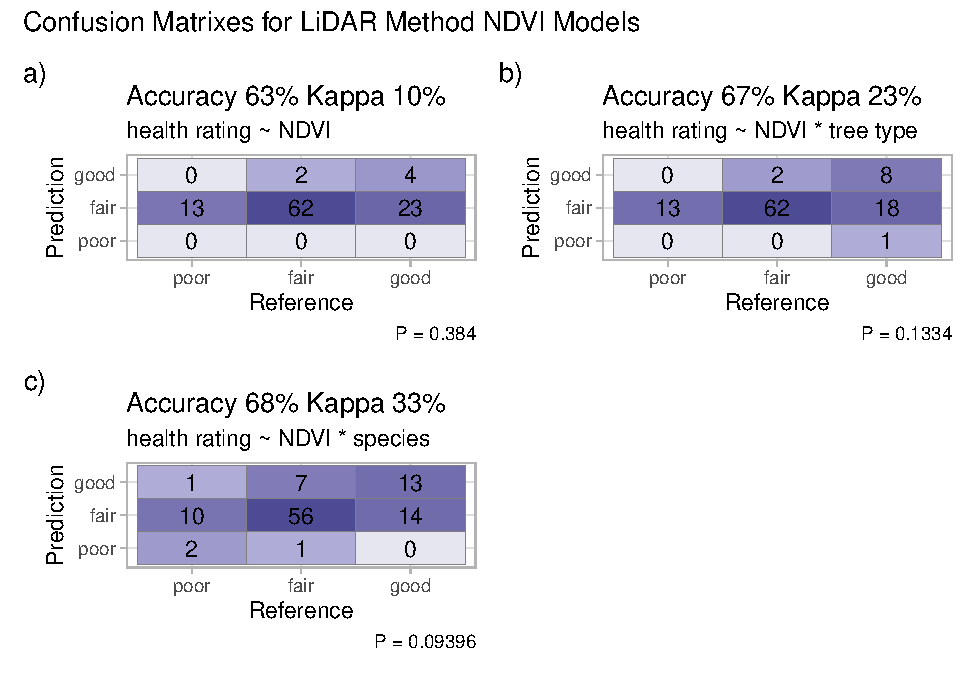
\includegraphics[width=0.9\linewidth,]{thesis_files/figure-latex/lidar-model-split-1} 

}

\caption[Confusion matrixes for LiDAR method predictive models]{Confusion matrixes for each species predictions with LiDAR method obtained NDVI values. (a) Model using NDVI to predict tree health category. (b) Model using functional tree type in addition to NDVI for health prediction. (c) Model with species as a predictor variable for NDVI based tree health category.}\label{fig:lidar-model-split}
\end{figure}
\begin{figure}[H]

{\centering 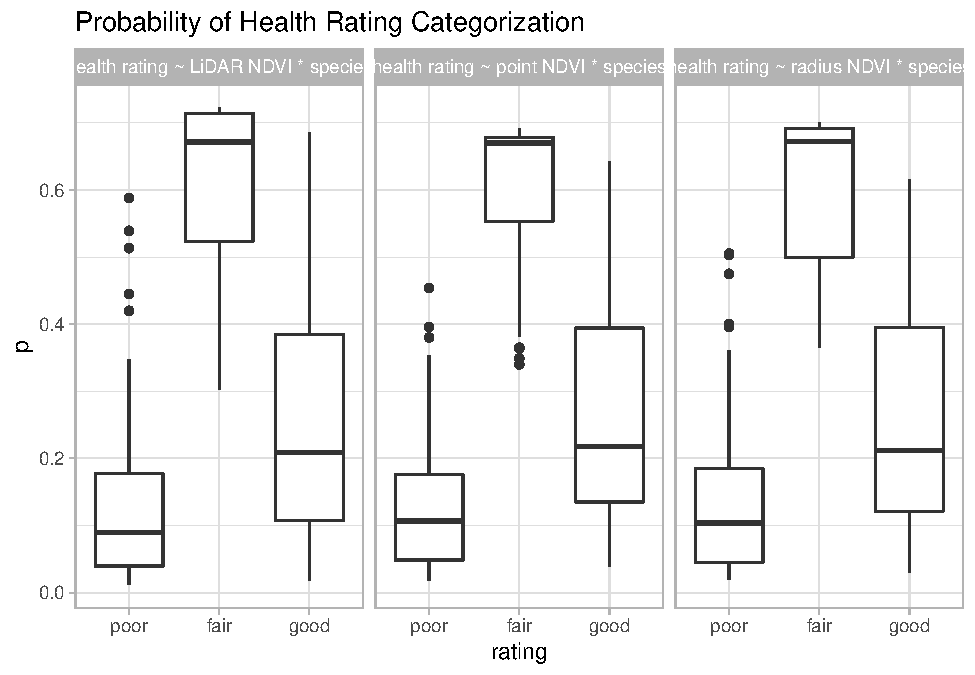
\includegraphics{thesis_files/figure-latex/prob-graph-1-1} 

}

\caption{Boxplot of probabilities of health group categorization}\label{fig:prob-graph-1}
\end{figure}
With the results of the models using species as an interaction term for
each of the three pixel selection methods (health rating \textasciitilde{} point NDVI
* species; health rating \textasciitilde{} radius NDVI * species; health rating \textasciitilde{}
LiDAR NDVI * species), I compared the probabilities of a given tree
being assigned each health category (Figure \ref{fig:prob-graph-1}).
For each prediction, a probability of assignment to each health category
is created (Table \ref{tab:preds-head}). The probability of a tree
being predicted as \textbf{good} stays fairly consistent across the three
methods, but the most interesting aspect is the probability of a
\textbf{poor} rating, which increases across models. This is consistent with
the confusion matrixes created for each model.

Given the uneven number of data points available for the varying health
conditions, I down-sampled each health rating to the smallest number of
points in a given category (Point = 15, Radius = 15, LiDAR = 13). When
the predictive models were ran with equal category sizes, the results
were statistically significant for all three pixel selection models. The
point and radius method models correctly predicted the health ratings
for most of the \textbf{poor} and \textbf{good} rated trees but not for \textbf{fair}
rated trees, which is the opposite of what we saw with the previous
models. The LiDAR model had the highest proportion of correctly
predicted health ratings across all three health categories (Figure
\ref{fig:final-model-small}).

I repeated the probability of assignment analysis with the downsampled
models (Figure \ref{fig:downsample-probs}). The probabilities of
assignment to each health category are much more even now, though the
average probability for a \textbf{fair} prediction is still higher than the
average probability of a \textbf{poor} or \textbf{good} rating prediction.
\begin{figure}[H]

{\centering 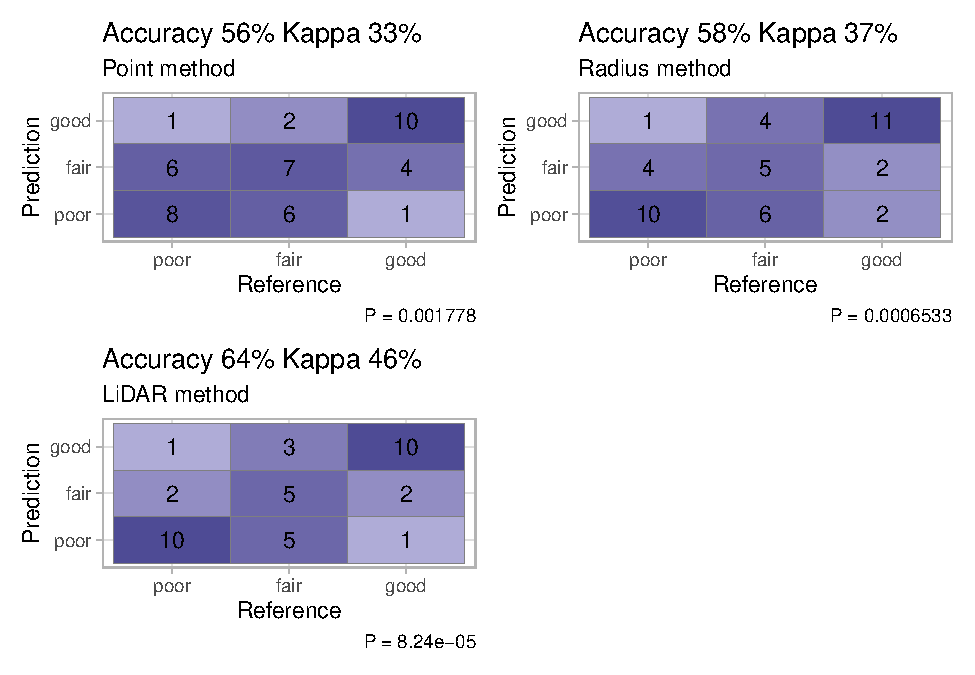
\includegraphics[width=0.9\linewidth,]{thesis_files/figure-latex/final-model-small-1} 

}

\caption{Confusion matrixes for downsampled predictive models}\label{fig:final-model-small}
\end{figure}
\begin{figure}[H]

{\centering 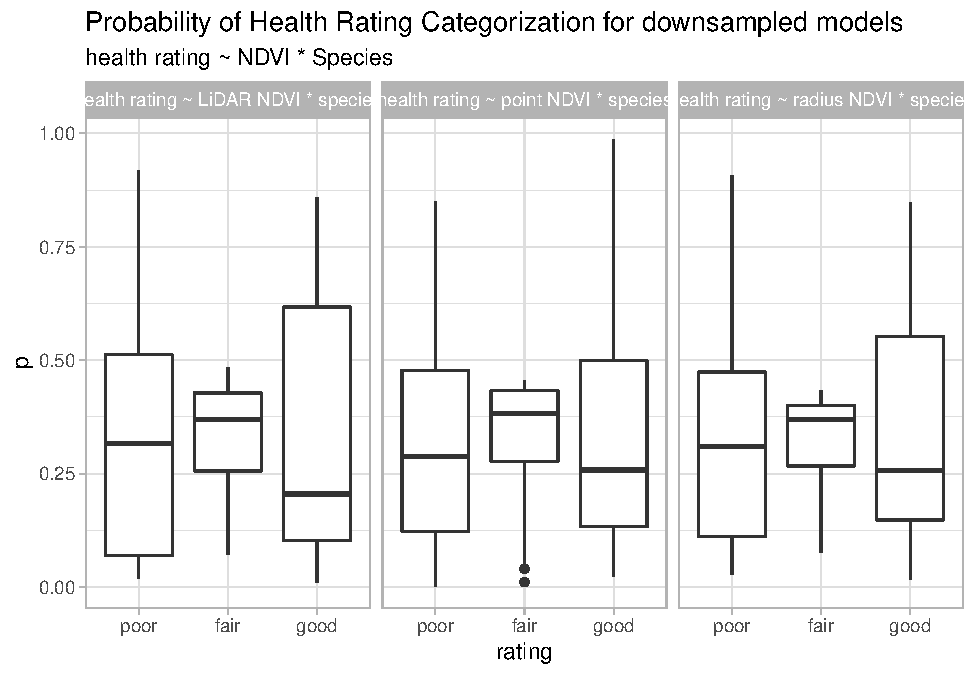
\includegraphics{thesis_files/figure-latex/downsample-probs-1} 

}

\caption{Probability of Assignment Analysis with Downsampled Data}\label{fig:downsample-probs}
\end{figure}
To ensure that the results of the downsampled LiDAR data model were not
caused by the random downsampling, I ran the model 6 times with
different random samples each time (Appendix
\ref{fig:lidar-model-test}). While the values of each predicted
category did differ, the p-value for the model was significant for each
test. The accuracy values ranged from 54\% to 67\%, and the kappa values
ranged from 31\% to 50\% (Table \ref{tab:model-test-table}).

\hypertarget{health-predictions-for-portland-trees}{%
\section{Health Predictions for Portland Trees}\label{health-predictions-for-portland-trees}}

I used the
final downsampled LiDAR model to predict health rating for a random
sample of 100 park and 100 street trees, with LiDAR calculated NDVI
values. Due to the data loss in the LiDAR processing, the final data set
contains 175 trees (85 street trees, 90 park trees) (Table
\ref{tab:final-lidar-counts}). This data was input into the final LiDAR
model, created with the downsampled data. A health rating was predicted
based on NDVI and tree species. The resulting health predictions were
graphed along with sample NDVI (Figure \ref{fig:final-lidar-plot}).
For ACMA, there is a clear relationship between sample NDVI and health
prediction which matches that seen in earlier data analysis. For ACPL,
there is a large difference between the NDVI of \textbf{fair} and \textbf{good}
trees, which also appears for PSME. for the THPL predictions, the
average NDVI for \textbf{poor} trees is higher than those for \textbf{fair} trees.
\begin{figure}[H]

{\centering 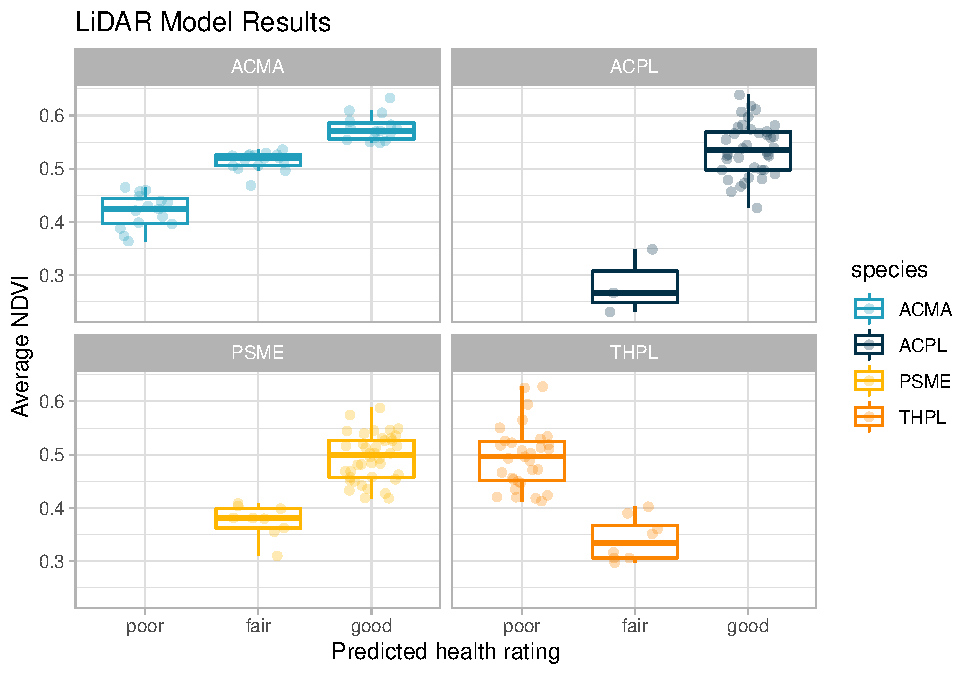
\includegraphics[width=0.9\linewidth,]{thesis_files/figure-latex/final-lidar-plot-1} 

}

\caption{Health rating predictions for random sample of Portland trees}\label{fig:final-lidar-plot}
\end{figure}
\hypertarget{discussion}{%
\chapter{Discussion}\label{discussion}}

The primary goals of this thesis were to investigate the impact of
functional type or species specification in predictive health models, as
well as an investigation of the impacts and outcomes of three different
pixel selection and tree crown delineation models. In summary, the
predictive models with species specificity as well as the models that
used NDVI data obtained through the LiDAR tree crown delineation had the
best results. However, each method had limitations despite their
effectiveness which will be discussed in further detail below.

\hypertarget{strengths-and-limitations-of-different-delineation-techniques}{%
\section{Strengths and limitations of different delineation techniques}\label{strengths-and-limitations-of-different-delineation-techniques}}

The three pixel selection methods (point, radius, and LiDAR) were used
to help answer the question \emph{which pixels are we using?} This was a
necessary part of this thesis methodology because in order to utilize
NDVI as a health metric, it was essential to select specific NDVI pixels
from satellite imagery for analysis. Three different methods of pixel
selection and tree crown delineation were tested: a point method which
used the single NDVI value from directly below a tree location point; a
radius method which averaged the NDVI values of all pixels contained
within a buffer circle defined by the measured or predicted tree crown
width; and a LiDAR method which used a modified watershed delineation
algorithm in conjunction with LiDAR canopy height model data to
delineate tree crowns into predicted polygon shapes (Figure
\ref{fig:layered-outputs-2}).
\begin{figure}[H]

{\centering 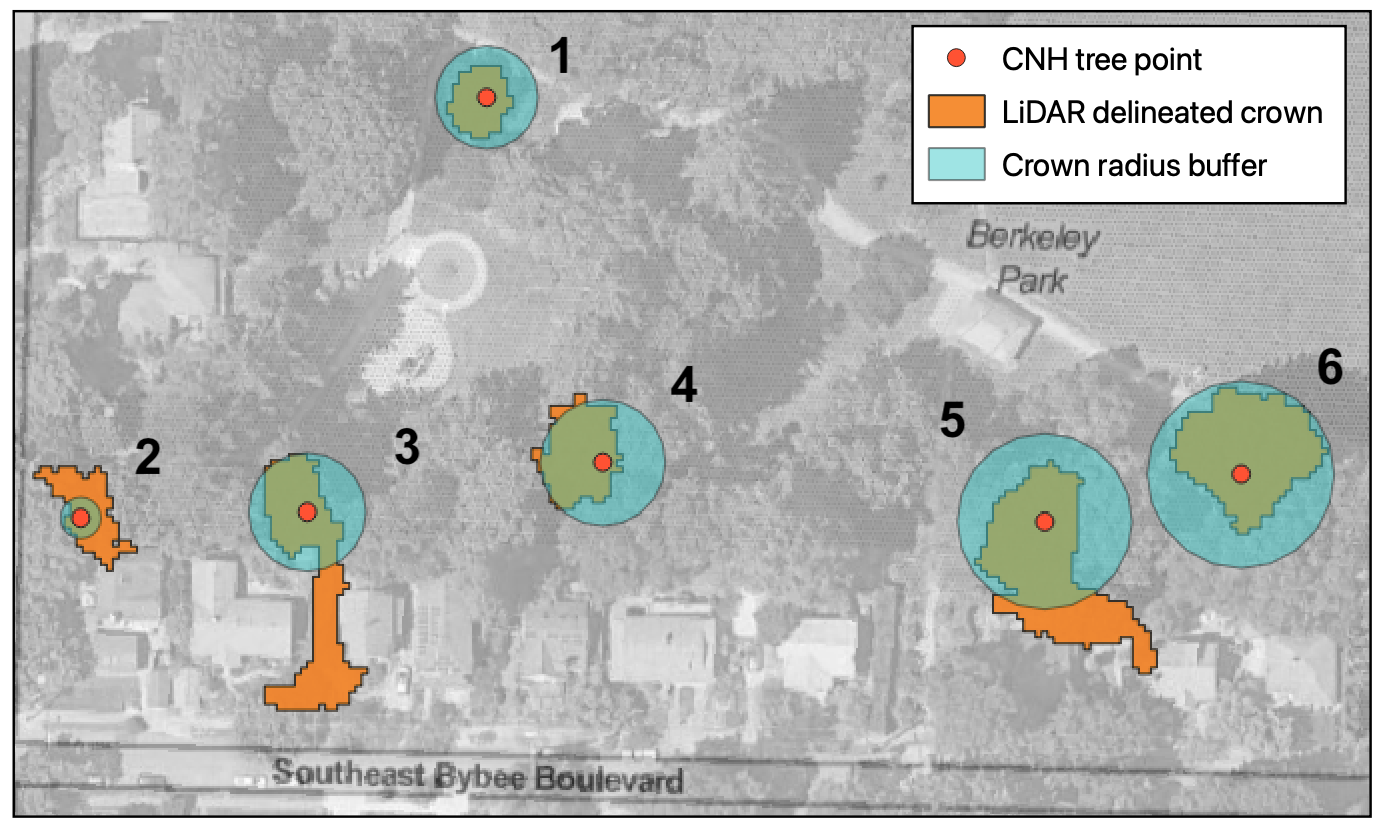
\includegraphics[width=0.9\linewidth,]{figure/layered_outputs_2} 

}

\caption[Pixel selection method comparison with numbered trees]{Point, Radius, and LiDAR pixel selection methods for Berkeley Park with numbered trees}\label{fig:layered-outputs-2}
\end{figure}
The single pixel point method results in an NDVI value representative
for the center-most section of a tree crown which may be effective for
small trees, but overlooks much of the data from the tree crown as a
whole, leading to this method being a poor representation of NDVI and
tree health for trees with larger canopies. The point method is the
simplest method, obtaining a single NDVI value from the individual pixel
that spatially contains an individual tree location point. The
statistically significant difference in the NDVI values for trees
categorized as \textbf{fair} and \textbf{good} seems to be primarily driven by the
THPL data (\ref{fig:point-species}). Given that only one pixel value is
used to represent the NDVI of an entire tree in the point method, that
single pixel likely misrepresents the health of the tree. If the
location point is incorrect, the NDVI value may not belong to the tree
of interest. The pixel method NDVI values statistically significantly
higher than the NDVI values obtained through the other two pixel
selection methods. This can be attributed to the use of a single pixel
rather than an average of pixel NDVI values. The approximated center of
the tree represented by the tree location point will generally be
greener than pixels on the edge because the NDVI value for a pixel is
the average NDVI for all data within that pixel, and the central pixel
likely contains mostly tree canopy, and ideally little to no information
on ground cover surrounding the tree. Because of this, the single pixel
point method is more likely to produce less ``noise'' within the data from
edge effects and non-canopy pixels. This is emphasized in figure
\ref{fig:layered-outputs-2}, which highlights the large variance in
pixel selection extent for the three methods and how much data is missed
by the point method. This model may be best for small trees or trees
that experience patterns of dieback positioned around their center and
trunk in contrast to the edges of the canopy. One of the main
limitations of the point method is the limited scope of data used in
analysis. However, this limitation does not exist for the radius method.

The radius method averages the NDVI values of pixels within a buffered
circle with the size defined by the measured or predicted tree canopy
width. This data had a statistically significant difference in average
NDVI values between \textbf{good} and \textbf{poor} categorized trees as well as
\textbf{good} and \textbf{fair} categorized trees (figure
\ref{fig:radius-species}). There is a larger difference between
\textbf{fair} and \textbf{good} than \textbf{fair} and \textbf{poor}, which is also seen in
the point method data. Where the scope of the pixel data is too narrow
(only using the value of a singular pixel) the scope of the radius
method can be too broad and pixels belonging to other trees will be
included. A large issue that can arise with the radius method data is
the overlapping of tree crowns, and pixels being used in the NDVI
analysis for multiple trees (Figure \ref{fig:overlap-crowns}).
Overlapping crowns is an issue that often arises with tree crown
delineation. To deal with this, Xiao et al. (2005) chose to exclude any trees
with overlapping crowns from the final analysis. Fang et al. (2020) used a
version of the radius method where they calculated an average canopy
width and used that standardized size (a radius of 4.55 m) to extract
their NDVI averages for each tree. The paper does not mention how they
dealt with overlapping tree crowns, but perhaps their trees were widely
distributed enough and the radius of interest was small enough that
their values did not experience overlap. Using LiDAR as a pixel
selection method has the benefit of additional pixel data like the
radius method, but no overlapping crowns.
\begin{figure}[H]

{\centering 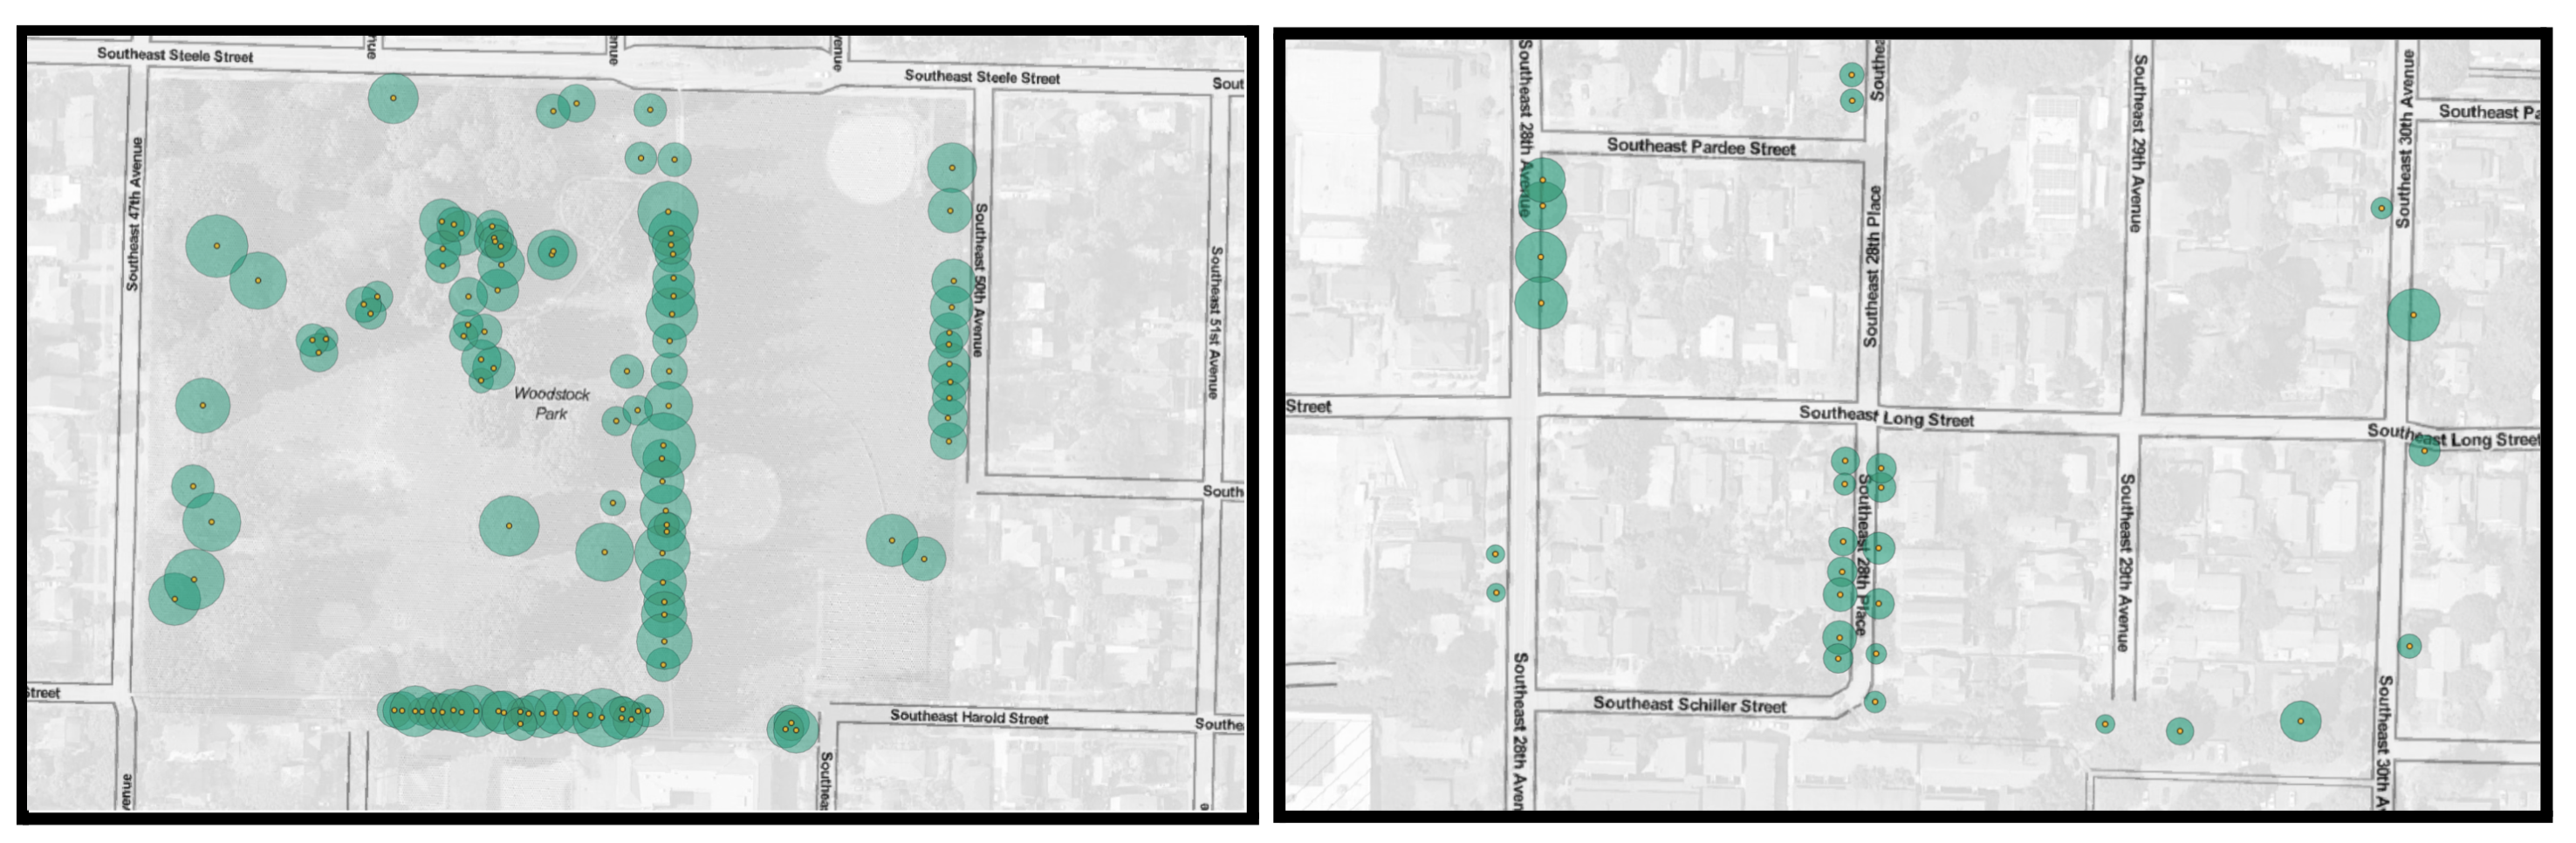
\includegraphics[width=1\linewidth,]{figure/overlapping-crowns} 

}

\caption[Examples of overlapping park and street tree crowns.]{Examples of tree crown buffers from radius method data with overlapping crowns for park trees (left) and street trees (right). While the frequency of overlapping crowns is much higehr for the park example, it is still apparent in the street trees as well. Given that these figures only include trees of the canary species, the occurance of overlapping tree canopies is likely even higher than this.}\label{fig:overlap-crowns}
\end{figure}
The LiDAR tree crown delineation was by far the most intensive pixel
selection method tested in this thesis, but was the most effective for
modeling purposes. In some cases (such as trees 1, 4, and 6 in figure
\ref{fig:layered-outputs-2}) the LiDAR delineation appears to be highly
effective in creating a polygon that is representative of a tree's
crown, without the inclusion of overlapping areas. However, there are
cases (such as trees 2, 3, and 5) where the canopy delineation algorithm
creates canopies for trees that are larger than reality. The LiDAR pixel
selection method also led to the most statistically significant
predictive models (\ref{fig:lidar-species}). Using LiDAR for canopy
delineation is complicated, but it is also quite effective.

Given the overall results of the three methods, I believe that the
radius and LiDAR methods are both valid choices for tree crown
delineation and pixel selection, but can have different intended uses
that will maximize the benefits of each model. The radius method is
fairly easy when compared to the LiDAR processing. It does have more
overlapping crowns, but fewer non-canopy pixels. Especially if the data
already contains a crown width measurement, the radius method can be a
decently simple method of selecting pixels for NDVI assessment. The
LiDAR method will not produce overlapping crowns but may include more
non-canopy pixels. If the goal is maximizing the accuracy of the tree
crown delineations, the the LiDAR method may be the best approach. A
future approach may be to use the LiDAR method to delineate tree crowns,
then trim the polygons based on the radius buffer to eliminate both
overlapping tree crowns as well as a majority of non-canopy pixels.

\hypertarget{evaluation-of-tree-health-predictions}{%
\section{Evaluation of Tree Health Predictions}\label{evaluation-of-tree-health-predictions}}

The final LiDAR model for predicting tree health based on NDVI and
species had promising results for the two maple species, especially
ACMA. The ACMA health predictions mirrored the pattern seen in the
measured health condition and LiDAR calculated NDVI. With ACPL, the
predictions showed effective separation of \textbf{fair} and \textbf{good}, but no
predictions of \textbf{poor} trees. A limitation for all of the models is
sample size. The models were only statistically significant when the
health rating groups were downsampled to equal sizes, and the accuracy
and kappa values varied depending on the sample of trees that was
included in the downsampled data (table \ref{tab:model-test-table}).
Additionally, the distribution of species across health rating with the
downsampled data is uneven (Table \ref{tab:species-counts-bleh}). Due
to data loss during the LiDAR canopy delineation, the final dataset used
for model training had no PSME individuals rated as \textbf{poor} health. In
the predictions, no PSME individuals were rated as \textbf{poor}, which in
context of the training dataset makes complete sense (Figure
\ref{fig:preds-counts}). If there is no basis for a prediction of a
specific health rating, that health rating will not be predicted. For
all species, an overall larger sample size would likely improve the
predictions and the model as a whole. This is easier said than done,
since while collecting field data and health analyses, the species
sampled can be controlled by selection, but their health cannot be. In
order to create a predictive model that works for more than just ACMA,
it is necessary to increase the size of data for model training.
\begin{table}

\caption{\label{tab:species-counts-bleh}Count of Species and Ratings in final dataset used for LiDAR downsampled model training}
\centering
\begin{tabular}[t]{lrrr}
\toprule
Species & Count Poor & Count Fair & Count Good\\
\midrule
ACMA & 6 & 3 & 2\\
ACPL & 2 & 2 & 9\\
THPL & 5 & 5 & 1\\
PSME & 0 & 3 & 1\\
\bottomrule
\end{tabular}
\end{table}
\hypertarget{impact-of-functional-tree-type-and-species-on-tree-health-assessments}{%
\section{Impact of Functional Tree Type and Species on Tree Health Assessments}\label{impact-of-functional-tree-type-and-species-on-tree-health-assessments}}

In all models and data analysis, very different patterns were seen
between the broadleaf deciduous trees (ACMA and ACPL) and the coniferous
evergreen trees (PSME and THPL). This is at least partially due to the
functional tree type and how these trees respond to environmental
conditions and declining health. Deciduous trees lose their leaves every
fall, and grow new ones every spring. Since their vegetation has a
shorter lifespan of one growing season, it is much more sensitive to
sudden and extreme environmental impacts. Declining health can be seen
in broadleaf trees as leaf damage or scorching, discoloration in the
foliage, or a decrease in the number of leaves grown each year.
Conversely, coniferous evergreen trees retain their foliage after each
growing season, adding new growth on to the end of branches. Since
evergreen trees cannot regrow all their foliage after a year with harsh
environmental conditions, their response is often seen in the loss of
branches and a reduction in overall canopy cover. Because of these
variations in response types, the models including functional type as a
predictor variable had higher levels of accuracy than the method only
using NDVI.

For each of the three pixel selection method models, the model that
differentiated the predictions by species was the most accurate. Because
of the differences in functional type and other species-specific
characteristics, it makes sense that increasing the specificity of the
model to species would improve the predictions. This additional
separation of tree species also highlighted the utility of the final
predictive model for separating ACMA individuals into distinct health
categories based on NDVI, but this did not hold true for the ACPL
predictions.

Separating the predictions by species was consistently more effective
than separating by functional type. Like with the tree crown
delineations, the species differentiation was the most effective, but
functional type specificity can do in a pinch. For the purpose of
obtaining a rough understanding of NDVI across various functional types
of trees, then specifying functional type instead of species will paint
an adequate picture of tree health. However, to maximize accuracy of
health predictions, species separation

\hypertarget{limitations-of-satellite-imaging}{%
\section{Limitations of Satellite Imaging}\label{limitations-of-satellite-imaging}}

While the use of satellite imaging for urban ecology applications is
becoming more frequent, there are still numerous avenues that need
additional research and improvement. The first of those is documentation
and access, which I will discuss further in the next section.

Another limitation of satellite imaging for tree health assessment is
seasonality. This limitation exists for field sampling as well, but must
be noted for remote sensing analysis. Especially with deciduous trees,
NDVI obtained outside of the peak growing season will not be able to get
anywhere close to an accurate health rating based on greenness. By
filtering for satellite images collected during the peak on-leaf period,
this variability can be limited. Fang et al. (2020) compared satellite images
from June, July, and August and found that the July image, which was
obtained for the peak on-leaf period for Washington D.C., was the most
accurate and effective when examining tree health.

Tree species also has a large impact on NDVI values due to the natural
variability in tree vegetation color. Coniferous trees are generally
much darker in color than deciduous trees. Between deciduous tree
species, there can be extensive variation in color as well. Some trees
have vegetation that naturally appears reddish or purple, so these
species would require a different type of vegetation index for health
modeling than species that are naturally quite green. Other vegetation
indices could be tested for their potential to better model the tree
health for coniferous trees.

While some of these limitations, such as seasonality, are inherent,
others that I experienced in this work were due to the type and
resolution of data that I was able to access. With higher resolution
satellite data, the NDVI values would be more specific to smaller areas
of the tree canopy, and could be used as part of the tree canopy
delineation as well. While there are numerous limitations of using
satellite imaging, the benefits do outweigh the limitations. The ability
to access and view data from past dates is invaluable. I hope that as
satellite data becomes more readily available to academics in the
future, it is also able to become more accessible to others in the
public sphere.

\hypertarget{open-source-data-and-accessible-science}{%
\section{Open Source Data and Accessible Science}\label{open-source-data-and-accessible-science}}

When beginning this thesis, a large goal of mine was to use only open
source and freely accessible data sources and programs. For much of the
thesis process, I thought I was meeting this goal. The satellite data I
used was accessed through PlanetScope's Education and Research Program,
which provided me with limited, non-commercial access to PlanetScope
satellite imagery. This is accessible after a short application,
provided that the applicant has a college or university email address.
This raises the question, is this truly an accessible data source? It
was free for me to use for this thesis, but I am able to do this thesis
and access the data because of the tuition I am playing to Reed College.

Both the street and park tree inventories were publicly available
through Portland's GIS opendata site, and the LiDAR canopy height model
was available through Portland's Regional Land Information System
(RLIS). The one processing task I was not able to do on an open source
software was the file conversion of the LiDAR CHM (canopy height model).
It is only available for download as a File Geodatabase, which is a
proprietary ArcGIS file type. In order to be able to utilize it in QGIS,
which is an opensource GIS software, I had to open the CHM file in
ArcGIS through Reed's institutional access, and export it as a \texttt{.tif}
file type. This is unfortunate, because it is very possible for
Portland's RLIS site to host the canopy height model in a different
format. However, in some ways the CHM may be more ``accessible'' than the
satellite data because even though it requires a proprietary software to
be able to use it, it is publicly accessible and anyone can download it.
While many of the data sources I used were openly accessible, throughout
this process it became apparent that the processing techniques were not.
I had to use three different platforms (RStudio, QGIS, and Python) to
conduct the work for this thesis for data analysis, mapping, and NDVI
processing of satellite data.

Satellite imagery with a 3m pixel size is relatively high resolution,
but less so in the context of urban ecology. The satellite data used in
Fang et al. (2020) was eight multispectral bands with a resolution of 1.2m, and
one panchromatic band with a spatial resolution of 0.3m. Satellite
imagery with this resolution or higher is unavailable to the public or
even for research purposes without payment or subscription to a data
hosting site. When I was working with PlanetScope data in the summer of
2020, I reached out to Planet Labs about gaining access to their higher
resolution data products and the possibility of purchasing individual
access to the data if needed. I was told that Planet does minimum
purchase orders of \$10,000 USD. While the availability of the basic
satellite imagery through Planet Labs is an incredible resource, it is
frustrating that the high price tag severely limits the accessibility of
much of their data.

While my goal was to use only publicly accessible data and open source
software for this thesis, in retrospect I realize that I was not
accessible. Many of the data sources I used had limitations or
restrictions that prevented them from being fully accessible. However,
that was out of my hands. I needed to use data for my thesis, and I was
lucky enough to have access to the data and software I needed.

\hypertarget{future-directions}{%
\section{Future Directions}\label{future-directions}}

For future work in modeling tree health, a combined pixel selection
using both the Radius and LiDAR methods could have promising results. By
calculating the areas of both the radius buffer circles and the LiDAR
canopies for each tree and using the smaller of the two areas, the
amount of overlapping tree crowns will be minimized along with the
overestimated LiDAR delineated crowns. Other studies have used an NDVI
threshold to exclude non-vegetation pixels, which was unrealistic to do
given the pixel size of the data I used. However, if this work could be
repeated with higher resolution NDVI data, masking of pixels based on an
NDVI threshold may be effective.

Additionally, altering the model to predict two conditions (\textbf{healthy}
vs \textbf{unhealthy}) may be more accurate, since all three pixel selection
methods had statistically significant differences between the \textbf{good}
and \textbf{fair} categories. This two condition model was used in Xiao et al. (2005).
Splitting the trees into two health categories instead of three would
increase the number of \textbf{unhealthy} trees predicted, since the trees
categorized as \textbf{fair} would be split between the \textbf{healthy} and
\textbf{unhealthy} ratings.

If I were able to continue this work, I would begin by conducting more
rigorous training and statistical testing on my predictive models. While
the polynomial models for tree height and crown width did have a
statistically better fit than the linear models, that was likely due to
over-fitting. I now believe that a linear model would have been a better
representation of the relationship seen in nature. A limitation of my
own work was the decision to train and test on the same dataset. While
the low sample size would still be an issue, bootstrapping or
cross-validation testing could be used to better fit the models without
over-fitting.

While there are many places that I know this thesis can be improved
upon, it still shows extremely promising results for the modeling of
urban maple species health in Portland, OR. While the species
specification and LiDAR delineation of may be time consuming and quite
involved, using the most specific method of tree specification and crown
delineation for pixel selection does provide the best results. The
ability to accurately predict health of urban trees from remotely sensed
data is an extremely important step towards understanding of urban
forest health dynamics so we can protect and maintain our urban forests.

\appendix

\hypertarget{data}{%
\chapter{Supplementary Data}\label{data}}

\hypertarget{additional-figures}{%
\section{Additional Figures}\label{additional-figures}}

\hypertarget{cnh-project-neighborhoods-and-classification}{%
\subsection*{CNH Project Neighborhoods and Classification}\label{cnh-project-neighborhoods-and-classification}}
\addcontentsline{toc}{subsection}{CNH Project Neighborhoods and Classification}
\begin{figure}[H]

{\centering 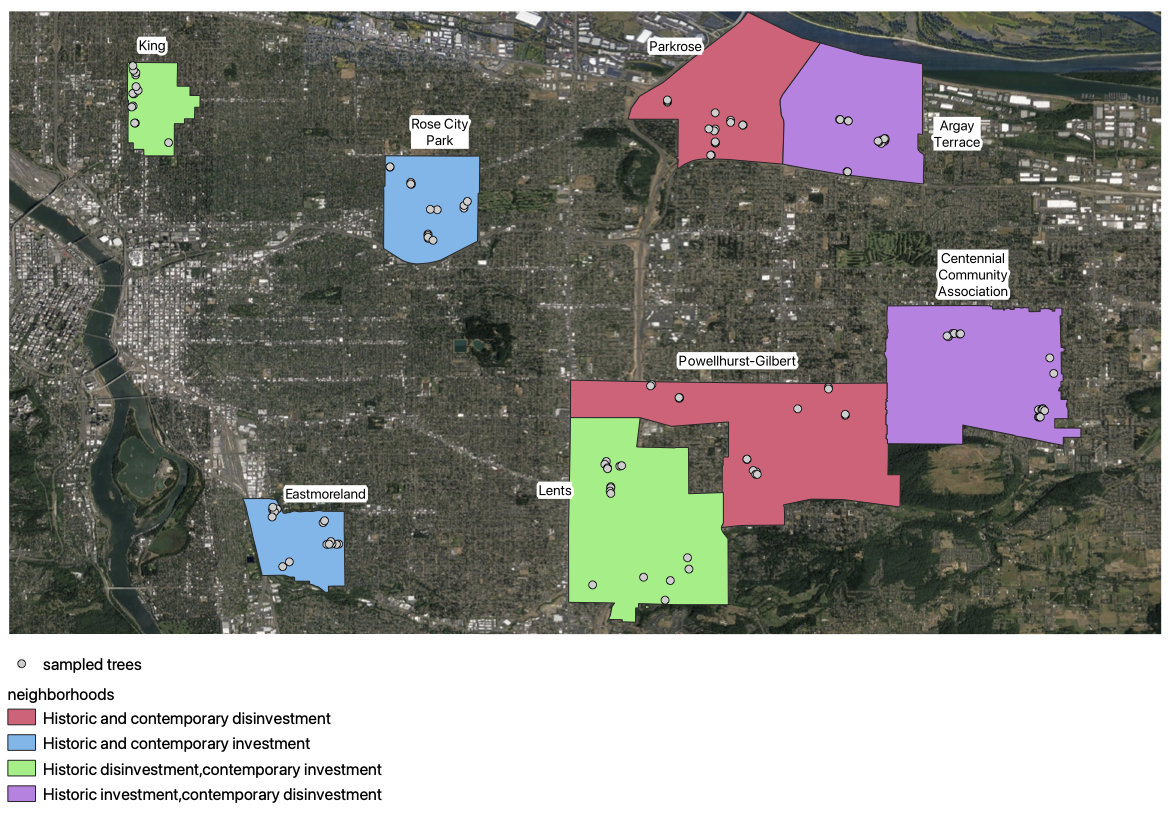
\includegraphics[width=1\linewidth,]{figure/neighborhoods_and_trees2} 

}

\caption{CNH sampled neighborhoods with classification}\label{fig:neighborhoods}
\end{figure}
\hypertarget{scene-products-and-satellite-swaths}{%
\subsection*{Scene products and satellite swaths}\label{scene-products-and-satellite-swaths}}
\addcontentsline{toc}{subsection}{Scene products and satellite swaths}
\begin{figure}[H]

{\centering \includegraphics[width=0.75\linewidth,]{figure/2016-bands} 

}

\caption{Satellite scene product swaths for 2016 PlanetScope data}\label{fig:2016-swath}
\end{figure}
\begin{figure}[H]

{\centering \includegraphics[width=0.75\linewidth,]{figure/2019-bands} 

}

\caption{Satellite scene product swaths for 2019 PlanetScope data}\label{fig:2019-swath}
\end{figure}
\begin{figure}[H]

{\centering \includegraphics[width=0.75\linewidth,]{figure/2021-bands} 

}

\caption{Satellite scene product swaths for 2021 PlanetScope data}\label{fig:2021-swath}
\end{figure}
\hypertarget{model-tests}{%
\subsection*{Model Tests}\label{model-tests}}
\addcontentsline{toc}{subsection}{Model Tests}
\begin{figure}[H]

{\centering 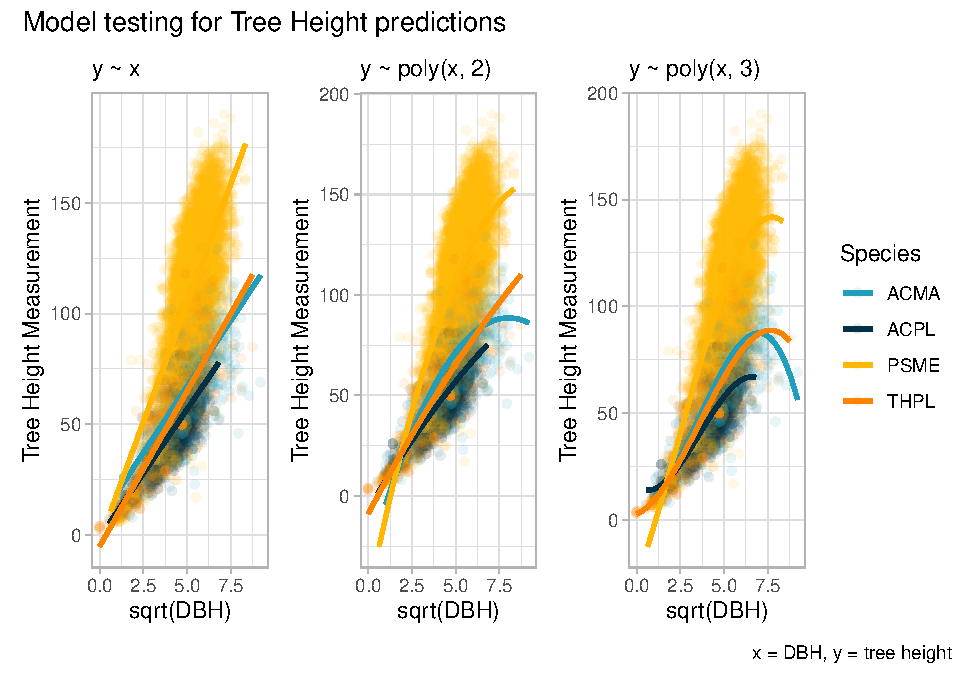
\includegraphics{thesis_files/figure-latex/test-height-model-1} 

}

\caption[Model tests for tree height predictions]{Predicting tree height from tree species and DBH. A linear, second degree, and third degree polynomial were tested, and raw polynomials were used.}\label{fig:test-height-model}
\end{figure}
\begin{figure}[H]

{\centering 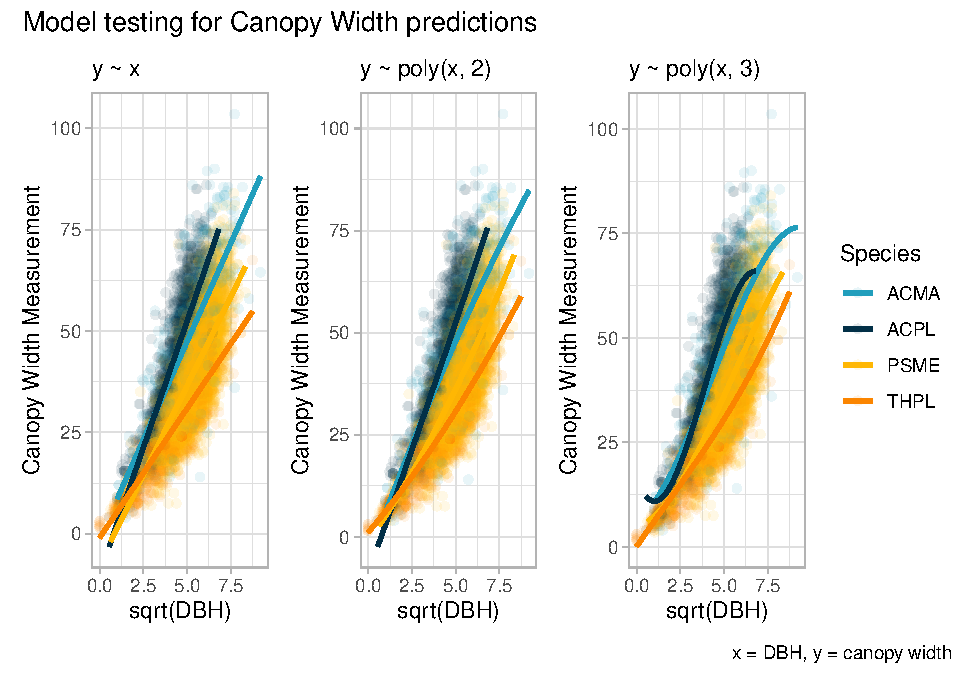
\includegraphics{thesis_files/figure-latex/test-width-model-1} 

}

\caption[Model tests for tree canopy width predictions]{Predicting canopy width from tree species and DBH. A linear, second degree, and third degree polynomial were tested, and raw polynomials were used.}\label{fig:test-width-model}
\end{figure}
\hypertarget{height-model-results-and-predictions}{%
\subsection*{Height model results and predictions}\label{height-model-results-and-predictions}}
\addcontentsline{toc}{subsection}{Height model results and predictions}
\begin{figure}[H]

{\centering 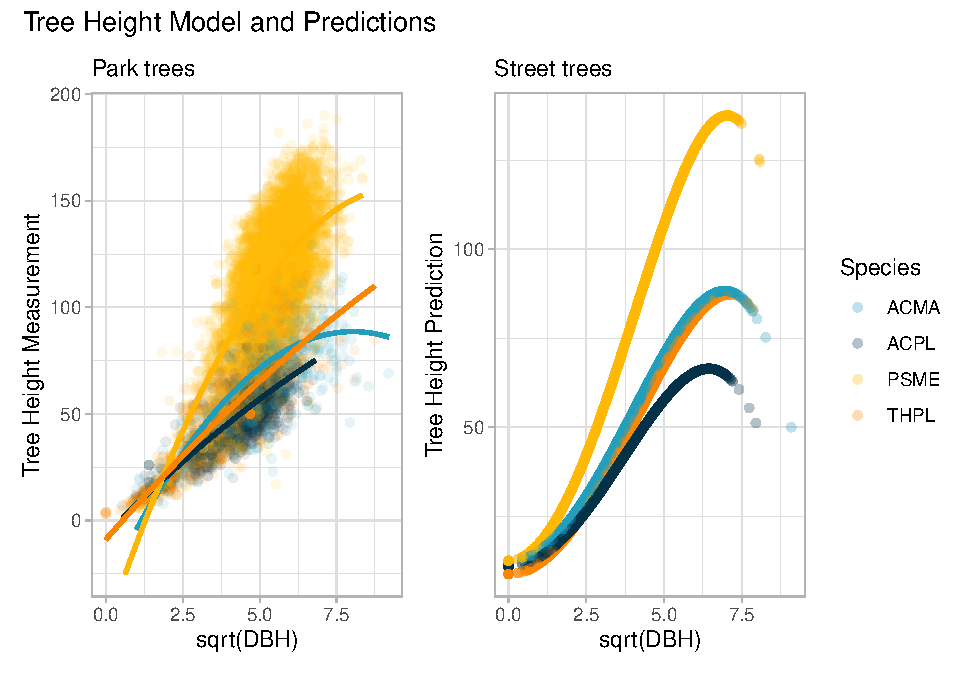
\includegraphics[width=0.8\linewidth,]{thesis_files/figure-latex/height-model-1} 

}

\caption[Tree height predictive model]{Predictive model for tree height from measured DBH. A second order polynomial regression was used in order to account for the variation between species. (Adjusted R-squared = 0.7834, P < 2.2e-16)}\label{fig:height-model}
\end{figure}
\hypertarget{lidar-model-tests}{%
\subsection*{LiDAR model tests}\label{lidar-model-tests}}
\addcontentsline{toc}{subsection}{LiDAR model tests}
\begin{figure}[H]

{\centering 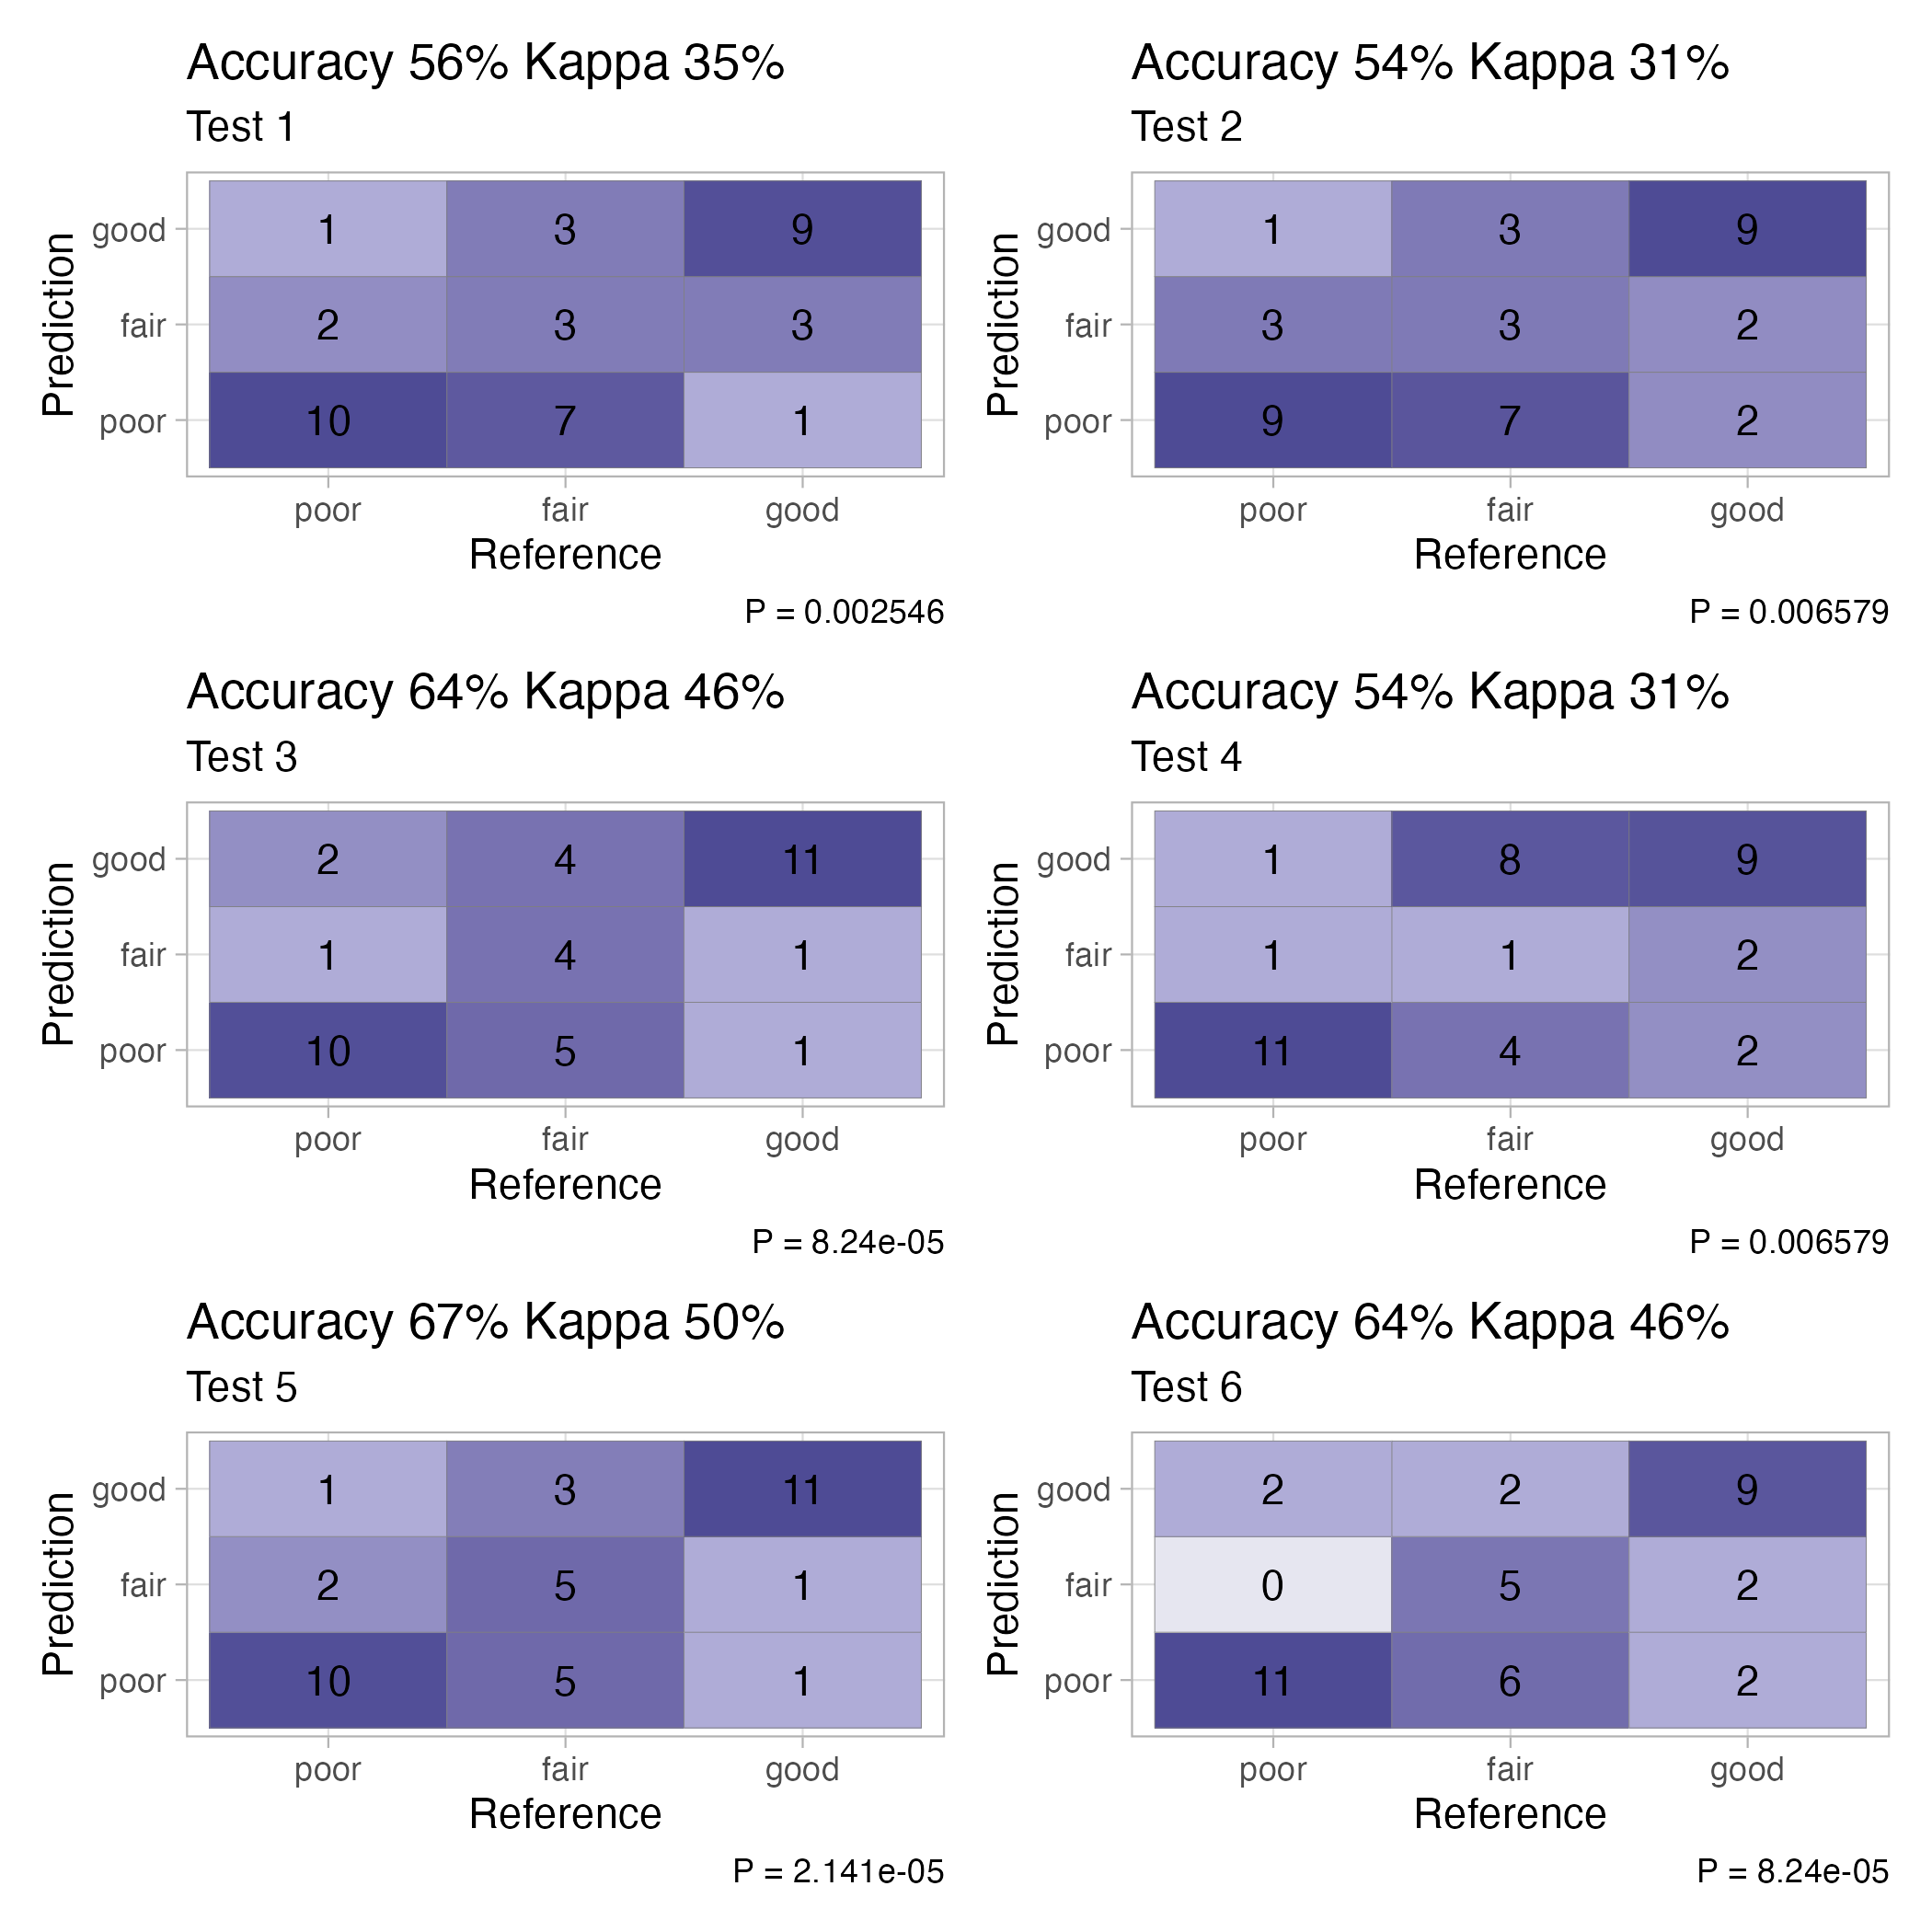
\includegraphics[width=1\linewidth,]{figure/test} 

}

\caption{Confusion matrixes for LiDAR predictive model tests}\label{fig:lidar-model-test}
\end{figure}
\hypertarget{predicted-health-rating-and-species-counts}{%
\subsection*{Predicted Health Rating and Species Counts}\label{predicted-health-rating-and-species-counts}}
\addcontentsline{toc}{subsection}{Predicted Health Rating and Species Counts}
\begin{figure}[H]

{\centering 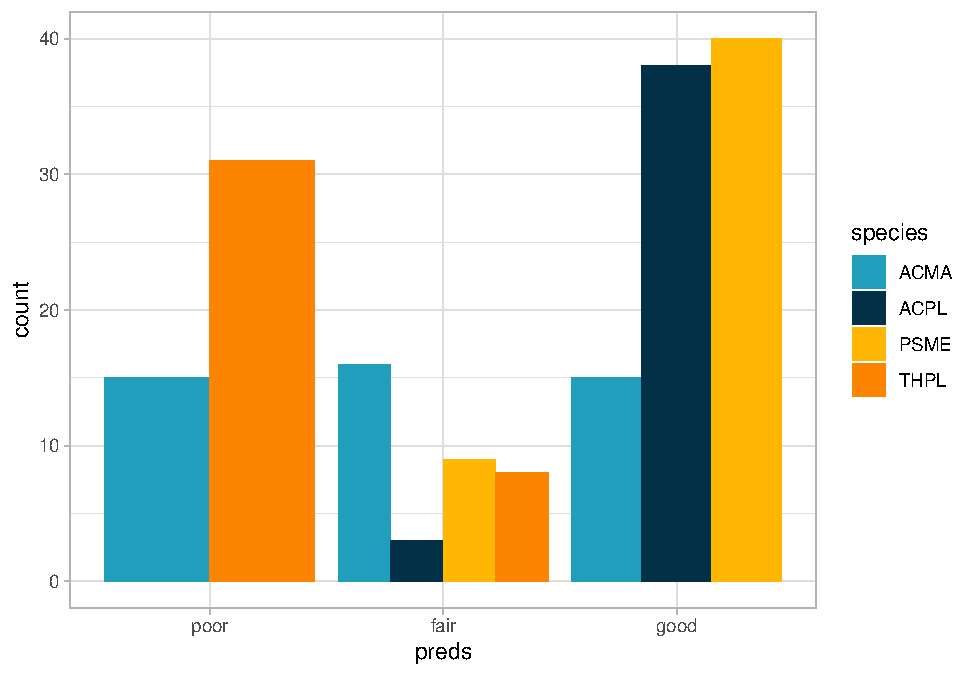
\includegraphics[width=0.9\linewidth,]{thesis_files/figure-latex/preds-counts-1} 

}

\caption{Graph of species counts for LiDAR health predictions}\label{fig:preds-counts}
\end{figure}
\hypertarget{additional-tables}{%
\section{Additional tables}\label{additional-tables}}

\hypertarget{variable-types-for-tree-inventories}{%
\subsection*{Variable types for tree inventories}\label{variable-types-for-tree-inventories}}
\addcontentsline{toc}{subsection}{Variable types for tree inventories}
\begin{longtable}[t]{llll}
\caption[Table of variables from tree inventory data]{\label{tab:var-type-table}Table of variables from the Portland park and street tree inventories, as well as sampled CNH variables.}\\
\toprule
Variable name & Street trees & Park trees & CNH2 trees\\
\midrule
\% canopy missing or dead & - & - & x\\
Address & x & - & -\\
Canopy base height & - & - & x\\
Carbon sequestration (lb) & - & x & -\\
Carbon sequestration (value) & - & x & -\\
\addlinespace
Carbon storage (lb) & - & x & -\\
Carbon storage (value) & - & x & -\\
Chlorophyll fluorescence & - & - & x\\
Common name & x & x & x\\
Crown width & - & x & x\\
\addlinespace
DBH & x & x & x\\
Edible (Y/N) & x & x & -\\
Evidence of injury, infestation, or disease & - & - & x\\
Evidence of watering & - & - & x\\
Family & x & x & x\\
\addlinespace
Foliage chrorophyll content & - & - & x\\
Foliage scorching & - & - & x\\
Functional type & x & x & -\\
Genus & x & x & x\\
Ground cover type & - & - & x\\
\addlinespace
Health Condition & x & x & x\\
Inventory Date & x & x & x\\
Leaf area index & - & - & x\\
Light level & - & - & x\\
Location (lat/long) & x & x & x\\
\addlinespace
Mature size (S/M/L) & x & x & -\\
Native (Y/N) & - & x & -\\
Nearest neighbor & - & - & x\\
Neighborhood & x & - & x\\
Nuisance (Y/N) & - & x & -\\
\addlinespace
Origin & - & x & -\\
Park name & - & x & x\\
Pollution removal (oz) & - & x & -\\
Pollution removal (value) & - & x & -\\
Presence of buildings within 25m & - & - & x\\
\addlinespace
Scientific name & x & x & x\\
Site development & x & - & -\\
Site size & x & - & -\\
Site type & x & - & x\\
Site width & x & - & -\\
\addlinespace
Species & x & x & x\\
Species factoid & - & x & -\\
Stomatal conductance & - & - & x\\
Stormwater (ft) & - & x & -\\
Stormwater (value) & - & x & -\\
\addlinespace
Structural value & - & x & -\\
Temperature (canopy, bole, air, ground) & - & - & x\\
Total annual services & - & x & -\\
Tree height & - & x & x\\
Volunteer or Staff? & x & x & -\\
\addlinespace
Wind speed & - & - & x\\
Wires (Y/N) & x & - & -\\
\bottomrule
\end{longtable}
\hypertarget{additional-information-on-health-predictive-model}{%
\subsection*{Additional Information on Health Predictive Model}\label{additional-information-on-health-predictive-model}}
\addcontentsline{toc}{subsection}{Additional Information on Health Predictive Model}
\begin{longtable}[t]{llllr}
\caption[Summary of results from various predictive models]{\label{tab:model-table}For each predictive model for tree health, this table contains the pixel selection method and predictors used, as well as the resulting accuracy, kappa, and p-value calculated in the confusion matrixes.}\\
\toprule
NDVI pixel method & Predictors & Accuracy & Kappa & P-value\\
\midrule
Point method & NDVI & 61\% & 0\% & 0.54120\\
Radius method & NDVI & 61\% & 3\% & 0.54120\\
LiDAR method & NDVI & 63\% & 10\% & 0.38400\\
Point method & NDVI * tree type & 63\% & 15\% & 0.31630\\
Radius method & NDVI * tree type & 63\% & 16\% & 0.31630\\
\addlinespace
LiDAR method & NDVI * tree type & 67\% & 23\% & 0.13340\\
Point method & NDVI * species & 64\% & 23\% & 0.25040\\
Radius method & NDVI * species & 64\% & 24\% & 0.25040\\
LiDAR method & NDVI * species & 68\% & 33\% & 0.09396\\
\bottomrule
\end{longtable}
\hypertarget{lidar-model-tests-1}{%
\subsection*{LiDAR model tests}\label{lidar-model-tests-1}}
\addcontentsline{toc}{subsection}{LiDAR model tests}
\begin{table}

\caption{\label{tab:model-test-table}Statistical values for LiDAR predictive model tests}
\centering
\begin{tabular}[t]{lllr}
\toprule
Test & Accuracy & Kappa & P-Value\\
\midrule
test 1 & 56\% & 35\% & 0.0025460\\
test 2 & 54\% & 31\% & 0.0065790\\
test 3 & 64\% & 46\% & 0.0000824\\
test 4 & 54\% & 31\% & 0.0065790\\
test 5 & 67\% & 50\% & 0.0000214\\
\addlinespace
test 6 & 64\% & 46\% & 0.0000824\\
\bottomrule
\end{tabular}
\end{table}
\hypertarget{prediction-probability-output-example}{%
\subsection*{Prediction Probability Output Example}\label{prediction-probability-output-example}}
\addcontentsline{toc}{subsection}{Prediction Probability Output Example}
\begin{table}[H]

\caption{\label{tab:preds-head}Selection of rows for LiDAR prediction probabilities}
\centering
\begin{tabular}[t]{rrr}
\toprule
poor & fair & good\\
\midrule
0.026 & 0.482 & 0.492\\
0.023 & 0.452 & 0.525\\
0.166 & 0.719 & 0.116\\
0.012 & 0.308 & 0.680\\
0.144 & 0.722 & 0.134\\
\bottomrule
\end{tabular}
\end{table}
\hypertarget{final-lidar-model-species-counts}{%
\subsection*{Final LiDAR Model Species Counts}\label{final-lidar-model-species-counts}}
\addcontentsline{toc}{subsection}{Final LiDAR Model Species Counts}
\begin{longtable}[t]{lr}
\caption[Species counts post LiDAR processing]{\label{tab:final-lidar-counts}Counts of each species in stratified random sample of park and street trees after LiDAR processing and NDVI calculation.}\\
\toprule
Species & Count\\
\midrule
ACMA & 46\\
ACPL & 41\\
PSME & 49\\
THPL & 39\\
\bottomrule
\end{longtable}
\hypertarget{additional-equations}{%
\section{Additional equations}\label{additional-equations}}

\hypertarget{tree-height-and-crown-width-predictive-model-equations}{%
\subsection*{Tree Height and Crown Width Predictive Model Equations}\label{tree-height-and-crown-width-predictive-model-equations}}
\addcontentsline{toc}{subsection}{Tree Height and Crown Width Predictive Model Equations}

\textbf{ACMA equations:} (\textit{x} = DBH)
\begin{equation}
\textrm{Tree Height} = 12.308 + 3.139x -0.032x^{2}  \\
\label{eq:a1}
\end{equation}
\begin{equation}
\textrm{Crown Width} = 12.117 + 1.721x - 0.0122x^{2} \\
\label{eq:a2}
\end{equation}
\textbf{ACPL equations:} (\textit{x} = DBH)
\begin{equation}
\textrm{Tree Height} = -1.359 - 0.464x + 0.000203x^2 \\
\label{eq:a3}
\end{equation}
\begin{equation}
\textrm{Crown Width} = -7.155 + 0.894x - 0.0153x^2 \\
\label{eq:a4}
\end{equation}
\textbf{PSME equations:} (\textit{x} = DBH)
\begin{equation}
\textrm{Tree Height} = 0.2448 + 1.916x - 0.0187x^2 \\
\label{eq:a5}
\end{equation}
\begin{equation}
\textrm{Crown Width} = -4.640583 - 0.3867x + 0.0046x^2 \\
\label{eq:a6}
\end{equation}
\textbf{THPL equations:} (\textit{x} = DBH)
\begin{equation}
\textrm{Tree Height} = -3.5146 - 0.0388x + 0.00178x^2 \\
\label{eq:a7}
\end{equation}
\begin{equation}
\textrm{Crown Width} = -4.953 - 0.5939x + 0.00512x^2 \\
\label{eq:a8}
\end{equation}
\hypertarget{code-chunks}{%
\chapter{Code}\label{code-chunks}}

This second appendix includes all of the R chunks of code that were
hidden throughout the document to help with readability and/or setup.

All code for this thesis can be found in my GitHub repository:
\url{https://github.com/zolli22/thesis_zoll}

\hypertarget{in-chapter-refdata-methods}{%
\section*{\texorpdfstring{\textbf{In Chapter} \ref{data-methods}\textbf{:}}{In Chapter \ref{data-methods}:}}\label{in-chapter-refdata-methods}}
\addcontentsline{toc}{section}{\textbf{In Chapter} \ref{data-methods}\textbf{:}}

\hypertarget{portland-tree-inventory-counts-and-calculations}{%
\subsection*{Portland Tree Inventory counts and calculations}\label{portland-tree-inventory-counts-and-calculations}}
\addcontentsline{toc}{subsection}{Portland Tree Inventory counts and calculations}

\footnotesize
\begin{Shaded}
\begin{Highlighting}[]
\NormalTok{street\_counts }\OtherTok{\textless{}{-}} \FunctionTok{get\_pdxTrees\_streets}\NormalTok{() }\SpecialCharTok{\%\textgreater{}\%}
    \FunctionTok{filter}\NormalTok{(Species }\SpecialCharTok{\%in\%} \FunctionTok{c}\NormalTok{(}\StringTok{"ACMA"}\NormalTok{, }\StringTok{"ACPL"}\NormalTok{, }\StringTok{"PSME"}\NormalTok{, }\StringTok{"THPL"}\NormalTok{)) }\SpecialCharTok{\%\textgreater{}\%}
    \FunctionTok{mutate}\NormalTok{(}\AttributeTok{year =} \FunctionTok{year}\NormalTok{(Inventory\_Date)) }\SpecialCharTok{\%\textgreater{}\%}
\NormalTok{    dplyr}\SpecialCharTok{::}\FunctionTok{select}\NormalTok{(Species, year) }\SpecialCharTok{\%\textgreater{}\%}
    \FunctionTok{add\_count}\NormalTok{(Species, year) }\SpecialCharTok{\%\textgreater{}\%}
    \FunctionTok{distinct}\NormalTok{() }\SpecialCharTok{\%\textgreater{}\%}
    \FunctionTok{group\_by}\NormalTok{(Species) }\SpecialCharTok{\%\textgreater{}\%}
    \FunctionTok{mutate}\NormalTok{(}\AttributeTok{Total =} \FunctionTok{sum}\NormalTok{(n)) }\SpecialCharTok{\%\textgreater{}\%}
    \FunctionTok{rename}\NormalTok{(}\AttributeTok{Count\_2016 =}\NormalTok{ n) }\SpecialCharTok{\%\textgreater{}\%}
    \FunctionTok{filter}\NormalTok{(year }\SpecialCharTok{==} \DecValTok{2016}\NormalTok{) }\SpecialCharTok{\%\textgreater{}\%}
\NormalTok{    dplyr}\SpecialCharTok{::}\FunctionTok{select}\NormalTok{(}\SpecialCharTok{{-}}\NormalTok{year)}

\NormalTok{park\_counts }\OtherTok{\textless{}{-}} \FunctionTok{get\_pdxTrees\_parks}\NormalTok{() }\SpecialCharTok{\%\textgreater{}\%}
    \FunctionTok{filter}\NormalTok{(Species }\SpecialCharTok{\%in\%} \FunctionTok{c}\NormalTok{(}\StringTok{"ACMA"}\NormalTok{, }\StringTok{"ACPL"}\NormalTok{, }\StringTok{"PSME"}\NormalTok{, }\StringTok{"THPL"}\NormalTok{)) }\SpecialCharTok{\%\textgreater{}\%}
    \FunctionTok{mutate}\NormalTok{(}\AttributeTok{year =} \FunctionTok{year}\NormalTok{(Inventory\_Date)) }\SpecialCharTok{\%\textgreater{}\%}
\NormalTok{    dplyr}\SpecialCharTok{::}\FunctionTok{select}\NormalTok{(Species, year) }\SpecialCharTok{\%\textgreater{}\%}
    \FunctionTok{add\_count}\NormalTok{(Species, year) }\SpecialCharTok{\%\textgreater{}\%}
    \FunctionTok{distinct}\NormalTok{() }\SpecialCharTok{\%\textgreater{}\%}
    \FunctionTok{group\_by}\NormalTok{(Species) }\SpecialCharTok{\%\textgreater{}\%}
    \FunctionTok{mutate}\NormalTok{(}\AttributeTok{Total =} \FunctionTok{sum}\NormalTok{(n)) }\SpecialCharTok{\%\textgreater{}\%}
    \FunctionTok{rename}\NormalTok{(}\AttributeTok{Count\_2019 =}\NormalTok{ n) }\SpecialCharTok{\%\textgreater{}\%}
    \FunctionTok{filter}\NormalTok{(year }\SpecialCharTok{==} \DecValTok{2019}\NormalTok{) }\SpecialCharTok{\%\textgreater{}\%}
\NormalTok{    dplyr}\SpecialCharTok{::}\FunctionTok{select}\NormalTok{(}\SpecialCharTok{{-}}\NormalTok{year)}
\end{Highlighting}
\end{Shaded}
\hypertarget{calculating-ndvi-from-satellite-imagery}{%
\subsection*{Calculating NDVI from satellite imagery}\label{calculating-ndvi-from-satellite-imagery}}
\addcontentsline{toc}{subsection}{Calculating NDVI from satellite imagery}

\footnotesize
\begin{Shaded}
\begin{Highlighting}[]
\NormalTok{import rasterio}
\NormalTok{import numpy}

\NormalTok{files }\OtherTok{=}\NormalTok{ [}\StringTok{"1"}\NormalTok{, }\StringTok{"2"}\NormalTok{, }\StringTok{"3"}\NormalTok{, }\StringTok{"4"}\NormalTok{] }\CommentTok{\# unique file identifiers}
\NormalTok{folder }\OtherTok{=} \StringTok{"ndvi\_calc\_thesis/files"} \CommentTok{\# folder with the raw files}
\NormalTok{date }\OtherTok{=} \StringTok{"20210726"} \CommentTok{\# product date}


\ControlFlowTok{for}\NormalTok{ i }\ControlFlowTok{in} \FunctionTok{range}\NormalTok{(}\FunctionTok{len}\NormalTok{(files))}\SpecialCharTok{:}
\NormalTok{    filenum }\OtherTok{=}\NormalTok{ files[i]}
\NormalTok{    image\_file }\OtherTok{=}\NormalTok{ folder}\SpecialCharTok{+}\StringTok{"/"}\SpecialCharTok{+}\NormalTok{date}\SpecialCharTok{+}\StringTok{"\_"}\SpecialCharTok{+}\NormalTok{filenum}\SpecialCharTok{+}\StringTok{"\_AnalyticMS.tif"}

\NormalTok{    metafile }\OtherTok{=}\NormalTok{ folder}\SpecialCharTok{+}\StringTok{"/"}\SpecialCharTok{+}\NormalTok{date}\SpecialCharTok{+}\StringTok{"\_"}\SpecialCharTok{+}\NormalTok{filenum}\SpecialCharTok{+}\StringTok{"\_AnalyticMS\_metadata.xml"}
    \FunctionTok{print}\NormalTok{(image\_file)}
    \FunctionTok{print}\NormalTok{(metafile)}

    \CommentTok{\# Load red and NIR bands {-} }
    \CommentTok{\# note all PlanetScope 4{-}band images have band order BGRN}

\NormalTok{    with }\FunctionTok{rasterio.open}\NormalTok{(image\_file) as src}\SpecialCharTok{:}
\NormalTok{        band\_red }\OtherTok{=} \FunctionTok{src.read}\NormalTok{(}\DecValTok{3}\NormalTok{)}

\NormalTok{    with }\FunctionTok{rasterio.open}\NormalTok{(image\_file) as src}\SpecialCharTok{:}
\NormalTok{        band\_nir }\OtherTok{=} \FunctionTok{src.read}\NormalTok{(}\DecValTok{4}\NormalTok{)}

\NormalTok{    from xml.dom import minidom}

\NormalTok{    xmldoc }\OtherTok{=} \FunctionTok{minidom.parse}\NormalTok{(metafile)}
\NormalTok{    nodes }\OtherTok{=} \FunctionTok{xmldoc.getElementsByTagName}\NormalTok{(}\StringTok{"ps:bandSpecificMetadata"}\NormalTok{)}

    \CommentTok{\# XML parser refers to bands by numbers 1{-}4}
\NormalTok{    coeffs }\OtherTok{=}\NormalTok{ \{\}}
    \ControlFlowTok{for}\NormalTok{ node }\ControlFlowTok{in}\NormalTok{ nodes}\SpecialCharTok{:}
\NormalTok{        bn }\OtherTok{=} \FunctionTok{node.getElementsByTagName}\NormalTok{(}\StringTok{"ps:bandNumber"}\NormalTok{)[}\DecValTok{0}\NormalTok{].firstChild.data}
        \ControlFlowTok{if}\NormalTok{ bn }\ControlFlowTok{in}\NormalTok{ [}\StringTok{\textquotesingle{}1\textquotesingle{}}\NormalTok{, }\StringTok{\textquotesingle{}2\textquotesingle{}}\NormalTok{, }\StringTok{\textquotesingle{}3\textquotesingle{}}\NormalTok{, }\StringTok{\textquotesingle{}4\textquotesingle{}}\NormalTok{]}\SpecialCharTok{:}
\NormalTok{            i }\OtherTok{=} \FunctionTok{int}\NormalTok{(bn)}
\NormalTok{            value }\OtherTok{=} \FunctionTok{node.getElementsByTagName}\NormalTok{(}\StringTok{"ps:reflectanceCoefficient"}\NormalTok{)[}\DecValTok{0}\NormalTok{].firstChild.data}
\NormalTok{            coeffs[i] }\OtherTok{=} \FunctionTok{float}\NormalTok{(value)}

    \CommentTok{\# Multiply by corresponding coefficients}
\NormalTok{    band\_red }\OtherTok{=}\NormalTok{ band\_red }\SpecialCharTok{*}\NormalTok{ coeffs[}\DecValTok{3}\NormalTok{]}
\NormalTok{    band\_nir }\OtherTok{=}\NormalTok{ band\_nir }\SpecialCharTok{*}\NormalTok{ coeffs[}\DecValTok{4}\NormalTok{]}

    \CommentTok{\# Allow division by zero}
    \FunctionTok{numpy.seterr}\NormalTok{(}\AttributeTok{divide=}\StringTok{\textquotesingle{}ignore\textquotesingle{}}\NormalTok{, }\AttributeTok{invalid=}\StringTok{\textquotesingle{}ignore\textquotesingle{}}\NormalTok{)}

    \CommentTok{\# Calculate NDVI}
\NormalTok{    ndvi }\OtherTok{=}\NormalTok{ (}\FunctionTok{band\_nir.astype}\NormalTok{(float) }\SpecialCharTok{{-}} \FunctionTok{band\_red.astype}\NormalTok{(float)) }\SpecialCharTok{/}\NormalTok{ (band\_nir }\SpecialCharTok{+}\NormalTok{ band\_red)}

    \CommentTok{\# Set spatial characteristics of the output object to mirror the input}
\NormalTok{    kwargs }\OtherTok{=}\NormalTok{ src.meta}
    \FunctionTok{kwargs.update}\NormalTok{(}
        \AttributeTok{dtype=}\NormalTok{rasterio.float32,}
        \AttributeTok{count=}\DecValTok{1}\NormalTok{)}
    
    \CommentTok{\# Set name for new NDVI file}
\NormalTok{    newfile }\OtherTok{=}\NormalTok{ folder }\SpecialCharTok{+} \StringTok{\textquotesingle{}/ndvi\_\textquotesingle{}} \SpecialCharTok{+}\NormalTok{ date }\SpecialCharTok{+} \StringTok{"\_"} \SpecialCharTok{+}\NormalTok{ filenum }\SpecialCharTok{+} \StringTok{\textquotesingle{}.tif\textquotesingle{}}

    \CommentTok{\# Create the file}
\NormalTok{    with }\FunctionTok{rasterio.open}\NormalTok{(newfile, }\StringTok{\textquotesingle{}w\textquotesingle{}}\NormalTok{, }\SpecialCharTok{**}\NormalTok{kwargs) as dst}\SpecialCharTok{:}
        \FunctionTok{dst.write\_band}\NormalTok{(}\DecValTok{1}\NormalTok{, }\FunctionTok{ndvi.astype}\NormalTok{(rasterio.float32))}
\end{Highlighting}
\end{Shaded}
\hypertarget{lidar-canopy-delineation}{%
\subsection*{LiDAR canopy delineation}\label{lidar-canopy-delineation}}
\addcontentsline{toc}{subsection}{LiDAR canopy delineation}

\footnotesize
\begin{Shaded}
\begin{Highlighting}[]
\FunctionTok{library}\NormalTok{(rgdal)}
\FunctionTok{library}\NormalTok{(imager)}
\FunctionTok{library}\NormalTok{(raster)}
\FunctionTok{library}\NormalTok{(ForestTools)}

\FunctionTok{options}\NormalTok{(}\AttributeTok{rgdal\_show\_exportToProj4\_warnings =} \StringTok{"none"}\NormalTok{)}

\DocumentationTok{\#\# Loading raster data}
\NormalTok{EML\_CHM }\OtherTok{\textless{}{-}} \FunctionTok{raster}\NormalTok{(}\StringTok{"\textasciitilde{}Desktop/thesis\_data/lidar\_crown/clipped\_lidar.tif"}\NormalTok{)}

\DocumentationTok{\#\# Loading tree points}
\NormalTok{all\_ttops }\OtherTok{\textless{}{-}} \FunctionTok{shapefile}\NormalTok{(}\StringTok{"\textasciitilde{}Desktop/thesis\_data/lidar\_crown/all\_tree\_points\_for\_delin.tif"}\NormalTok{)}

\CommentTok{\# delineate tree crowns inputs: my tree points, LiDAR data}
\NormalTok{crownsPoly }\OtherTok{\textless{}{-}} \FunctionTok{mcws}\NormalTok{(}\AttributeTok{treetops =}\NormalTok{ all\_ttops, }\AttributeTok{CHM =}\NormalTok{ EML\_CHM, }\AttributeTok{format =} \StringTok{"polygons"}\NormalTok{,}
    \AttributeTok{minHeight =} \DecValTok{20}\NormalTok{, }\AttributeTok{verbose =} \ConstantTok{TRUE}\NormalTok{)}

\CommentTok{\# export file}
\FunctionTok{writeOGR}\NormalTok{(crownsPoly, }\StringTok{"\textasciitilde{}/Desktop/thesis\_data/lidar\_crown"}\NormalTok{, }\StringTok{"canopy\_delin\_polygons\_poly"}\NormalTok{,}
    \AttributeTok{driver =} \StringTok{"ESRI Shapefile"}\NormalTok{)}
\end{Highlighting}
\end{Shaded}
\hypertarget{in-chapter-refresults}{%
\section*{\texorpdfstring{\textbf{In Chapter} \ref{results}\textbf{:}}{In Chapter \ref{results}:}}\label{in-chapter-refresults}}
\addcontentsline{toc}{section}{\textbf{In Chapter} \ref{results}\textbf{:}}

\hypertarget{model-for-tree-height-and-canopy-width}{%
\subsection*{Model for Tree Height and Canopy Width}\label{model-for-tree-height-and-canopy-width}}
\addcontentsline{toc}{subsection}{Model for Tree Height and Canopy Width}

\footnotesize
\begin{Shaded}
\begin{Highlighting}[]
\CommentTok{\# create model for heights}
\NormalTok{heights }\OtherTok{\textless{}{-}} \FunctionTok{lm}\NormalTok{(Tree\_Height }\SpecialCharTok{\textasciitilde{}} \FunctionTok{poly}\NormalTok{(DBH, }\AttributeTok{degree =} \DecValTok{2}\NormalTok{, }\AttributeTok{raw =}\NormalTok{ T) }\SpecialCharTok{*}
\NormalTok{    Species, }\AttributeTok{data =}\NormalTok{ my\_park)}
\FunctionTok{summary}\NormalTok{(heights)}

\CommentTok{\# create model for crown width}
\NormalTok{cr\_width }\OtherTok{\textless{}{-}} \FunctionTok{lm}\NormalTok{(crown\_width }\SpecialCharTok{\textasciitilde{}} \FunctionTok{poly}\NormalTok{(DBH, }\AttributeTok{degree =} \DecValTok{2}\NormalTok{, }\AttributeTok{raw =}\NormalTok{ T) }\SpecialCharTok{*}
\NormalTok{    Species, }\AttributeTok{data =}\NormalTok{ my\_park)}
\FunctionTok{summary}\NormalTok{(cr\_width)}

\CommentTok{\# load street data, filter to relevant species}
\NormalTok{my\_street }\OtherTok{\textless{}{-}}\NormalTok{ pdxTrees}\SpecialCharTok{::}\FunctionTok{get\_pdxTrees\_streets}\NormalTok{() }\SpecialCharTok{\%\textgreater{}\%}
    \FunctionTok{filter}\NormalTok{(Species }\SpecialCharTok{\%in\%} \FunctionTok{c}\NormalTok{(}\StringTok{"ACPL"}\NormalTok{, }\StringTok{"THPL"}\NormalTok{, }\StringTok{"PSME"}\NormalTok{, }\StringTok{"ACMA"}\NormalTok{))}

\CommentTok{\# run street trees through both models}
\NormalTok{my\_street\_2 }\OtherTok{\textless{}{-}}\NormalTok{ my\_street }\SpecialCharTok{\%\textgreater{}\%}
    \FunctionTok{mutate}\NormalTok{(}\AttributeTok{width\_preds =} \FunctionTok{predict}\NormalTok{(cr\_width, my\_street, }\AttributeTok{se.fit =} \ConstantTok{FALSE}\NormalTok{),}
        \AttributeTok{height\_preds =} \FunctionTok{predict}\NormalTok{(heights, my\_street, }\AttributeTok{se.fit =}\NormalTok{ F))}

\CommentTok{\# export data file write\_csv(my\_street,}
\CommentTok{\# \textquotesingle{}data/my\_street\_2.csv\textquotesingle{})}

\CommentTok{\# graphing}
\NormalTok{p\_height\_model }\OtherTok{\textless{}{-}}\NormalTok{ my\_park }\SpecialCharTok{\%\textgreater{}\%}
    \FunctionTok{ggplot}\NormalTok{(}\FunctionTok{aes}\NormalTok{(}\AttributeTok{x =} \FunctionTok{sqrt}\NormalTok{(DBH), }\AttributeTok{y =}\NormalTok{ Tree\_Height, }\AttributeTok{color =}\NormalTok{ Species)) }\SpecialCharTok{+}
    \FunctionTok{geom\_point}\NormalTok{(}\AttributeTok{alpha =} \FloatTok{0.1}\NormalTok{) }\SpecialCharTok{+} \FunctionTok{scale\_color\_manual}\NormalTok{(}\AttributeTok{values =}\NormalTok{ species\_pal) }\SpecialCharTok{+}
    \FunctionTok{geom\_smooth}\NormalTok{(}\AttributeTok{method =} \StringTok{"lm"}\NormalTok{, }\AttributeTok{se =}\NormalTok{ F, }\AttributeTok{formula =}\NormalTok{ y }\SpecialCharTok{\textasciitilde{}} \FunctionTok{poly}\NormalTok{(x,}
        \AttributeTok{degree =} \DecValTok{2}\NormalTok{, }\AttributeTok{raw =}\NormalTok{ T)) }\SpecialCharTok{+} \FunctionTok{labs}\NormalTok{(}\AttributeTok{subtitle =} \StringTok{"Measurements from park trees"}\NormalTok{,}
    \AttributeTok{y =} \StringTok{"Tree Height Measurement"}\NormalTok{, }\AttributeTok{title =} \StringTok{"Model"}\NormalTok{) }\SpecialCharTok{+} \FunctionTok{guides}\NormalTok{(}\AttributeTok{color =} \StringTok{"none"}\NormalTok{)}

\NormalTok{p\_width\_model }\OtherTok{\textless{}{-}}\NormalTok{ my\_park }\SpecialCharTok{\%\textgreater{}\%}
    \FunctionTok{ggplot}\NormalTok{(}\FunctionTok{aes}\NormalTok{(}\AttributeTok{x =} \FunctionTok{sqrt}\NormalTok{(DBH), }\AttributeTok{y =}\NormalTok{ crown\_width, }\AttributeTok{color =}\NormalTok{ Species)) }\SpecialCharTok{+}
    \FunctionTok{geom\_point}\NormalTok{(}\AttributeTok{alpha =} \FloatTok{0.1}\NormalTok{) }\SpecialCharTok{+} \FunctionTok{scale\_color\_manual}\NormalTok{(}\AttributeTok{values =}\NormalTok{ species\_pal) }\SpecialCharTok{+}
    \FunctionTok{geom\_smooth}\NormalTok{(}\AttributeTok{method =} \StringTok{"lm"}\NormalTok{, }\AttributeTok{se =}\NormalTok{ F, }\AttributeTok{formula =}\NormalTok{ y }\SpecialCharTok{\textasciitilde{}} \FunctionTok{poly}\NormalTok{(x,}
        \AttributeTok{degree =} \DecValTok{2}\NormalTok{, }\AttributeTok{raw =}\NormalTok{ T)) }\SpecialCharTok{+} \FunctionTok{labs}\NormalTok{(}\AttributeTok{subtitle =} \StringTok{"Measurements from park trees"}\NormalTok{,}
    \AttributeTok{y =} \StringTok{"Canopy Width Measurement"}\NormalTok{, }\AttributeTok{title =} \StringTok{"Model"}\NormalTok{) }\SpecialCharTok{+} \FunctionTok{guides}\NormalTok{(}\AttributeTok{color =} \StringTok{"none"}\NormalTok{)}

\NormalTok{s\_height\_preds }\OtherTok{\textless{}{-}}\NormalTok{ my\_street\_2 }\SpecialCharTok{\%\textgreater{}\%}
    \FunctionTok{ggplot}\NormalTok{(}\FunctionTok{aes}\NormalTok{(}\AttributeTok{x =} \FunctionTok{sqrt}\NormalTok{(DBH), }\AttributeTok{y =}\NormalTok{ height\_preds, }\AttributeTok{color =}\NormalTok{ Species)) }\SpecialCharTok{+}
    \FunctionTok{geom\_point}\NormalTok{(}\AttributeTok{alpha =} \FloatTok{0.3}\NormalTok{) }\SpecialCharTok{+} \FunctionTok{scale\_color\_manual}\NormalTok{(}\AttributeTok{values =}\NormalTok{ species\_pal) }\SpecialCharTok{+}
    \FunctionTok{labs}\NormalTok{(}\AttributeTok{subtitle =} \StringTok{"Predictions for street trees"}\NormalTok{, }\AttributeTok{y =} \StringTok{"Tree Height Prediction"}\NormalTok{,}
        \AttributeTok{title =} \StringTok{"Predictions"}\NormalTok{)}

\NormalTok{s\_width\_preds }\OtherTok{\textless{}{-}}\NormalTok{ my\_street\_2 }\SpecialCharTok{\%\textgreater{}\%}
    \FunctionTok{ggplot}\NormalTok{(}\FunctionTok{aes}\NormalTok{(}\AttributeTok{x =} \FunctionTok{sqrt}\NormalTok{(DBH), }\AttributeTok{y =}\NormalTok{ width\_preds, }\AttributeTok{color =}\NormalTok{ Species)) }\SpecialCharTok{+}
    \FunctionTok{geom\_point}\NormalTok{(}\AttributeTok{alpha =} \FloatTok{0.3}\NormalTok{) }\SpecialCharTok{+} \FunctionTok{scale\_color\_manual}\NormalTok{(}\AttributeTok{values =}\NormalTok{ species\_pal) }\SpecialCharTok{+}
    \FunctionTok{labs}\NormalTok{(}\AttributeTok{subtitle =} \StringTok{"Predictions for street trees"}\NormalTok{, }\AttributeTok{y =} \StringTok{"Canopy Width Prediction"}\NormalTok{,}
        \AttributeTok{title =} \StringTok{"Predictions"}\NormalTok{)}
\end{Highlighting}
\end{Shaded}
\hypertarget{point-method-modeling}{%
\subsection*{Point Method Modeling}\label{point-method-modeling}}
\addcontentsline{toc}{subsection}{Point Method Modeling}

\footnotesize
\begin{Shaded}
\begin{Highlighting}[]
\NormalTok{point\_all }\OtherTok{\textless{}{-}} \FunctionTok{polr}\NormalTok{(health\_rat }\SpecialCharTok{\textasciitilde{}}\NormalTok{ sample\_ndvi, }\AttributeTok{Hess =} \ConstantTok{TRUE}\NormalTok{, }\AttributeTok{data =}\NormalTok{ cnh\_point)}
\NormalTok{brant}\SpecialCharTok{::}\FunctionTok{brant}\NormalTok{(point\_all)}

\NormalTok{point\_all\_preds }\OtherTok{\textless{}{-}} \FunctionTok{predict}\NormalTok{(point\_all, cnh\_point)}
\NormalTok{cfm\_p\_all }\OtherTok{\textless{}{-}} \FunctionTok{confusionMatrix}\NormalTok{(point\_all\_preds, cnh\_point}\SpecialCharTok{$}\NormalTok{health\_rat)}

\NormalTok{p\_all }\OtherTok{\textless{}{-}} \FunctionTok{ggplotConfusionMatrix}\NormalTok{(cfm\_p\_all)}

\NormalTok{point\_type }\OtherTok{\textless{}{-}} \FunctionTok{polr}\NormalTok{(health\_rat }\SpecialCharTok{\textasciitilde{}}\NormalTok{ sample\_ndvi }\SpecialCharTok{*}\NormalTok{ tree\_type, }\AttributeTok{Hess =} \ConstantTok{TRUE}\NormalTok{,}
    \AttributeTok{data =}\NormalTok{ cnh\_point)}
\NormalTok{brant}\SpecialCharTok{::}\FunctionTok{brant}\NormalTok{(point\_type)}

\NormalTok{point\_type\_preds }\OtherTok{\textless{}{-}} \FunctionTok{predict}\NormalTok{(point\_type, cnh\_point)}
\NormalTok{cfm\_p\_type }\OtherTok{\textless{}{-}} \FunctionTok{confusionMatrix}\NormalTok{(point\_type\_preds, cnh\_point}\SpecialCharTok{$}\NormalTok{health\_rat)}

\NormalTok{p\_type }\OtherTok{\textless{}{-}} \FunctionTok{ggplotConfusionMatrix}\NormalTok{(cfm\_p\_type)}

\NormalTok{point\_species }\OtherTok{\textless{}{-}} \FunctionTok{polr}\NormalTok{(health\_rat }\SpecialCharTok{\textasciitilde{}}\NormalTok{ sample\_ndvi }\SpecialCharTok{*}\NormalTok{ species, }\AttributeTok{Hess =} \ConstantTok{TRUE}\NormalTok{,}
    \AttributeTok{data =}\NormalTok{ cnh\_point)}
\NormalTok{brant}\SpecialCharTok{::}\FunctionTok{brant}\NormalTok{(point\_species)}

\NormalTok{point\_species\_preds }\OtherTok{\textless{}{-}} \FunctionTok{predict}\NormalTok{(point\_species, cnh\_point)}
\NormalTok{cfm\_p\_species }\OtherTok{\textless{}{-}} \FunctionTok{confusionMatrix}\NormalTok{(point\_species\_preds, cnh\_point}\SpecialCharTok{$}\NormalTok{health\_rat)}

\NormalTok{p\_species }\OtherTok{\textless{}{-}} \FunctionTok{ggplotConfusionMatrix}\NormalTok{(cfm\_p\_species)}
\end{Highlighting}
\end{Shaded}
\hypertarget{radius-method-modeling}{%
\subsection*{Radius Method Modeling}\label{radius-method-modeling}}
\addcontentsline{toc}{subsection}{Radius Method Modeling}

\footnotesize
\begin{Shaded}
\begin{Highlighting}[]
\NormalTok{radius\_all }\OtherTok{\textless{}{-}} \FunctionTok{polr}\NormalTok{(health\_rat }\SpecialCharTok{\textasciitilde{}}\NormalTok{ sample\_ndvi, }\AttributeTok{Hess =} \ConstantTok{TRUE}\NormalTok{, }\AttributeTok{data =}\NormalTok{ cnh\_radius)}
\NormalTok{radius\_all\_preds }\OtherTok{\textless{}{-}} \FunctionTok{predict}\NormalTok{(radius\_all, cnh\_radius)}
\NormalTok{cfm\_r\_all }\OtherTok{\textless{}{-}} \FunctionTok{confusionMatrix}\NormalTok{(radius\_all\_preds, cnh\_radius}\SpecialCharTok{$}\NormalTok{health\_rat)}
\NormalTok{r\_all }\OtherTok{\textless{}{-}} \FunctionTok{ggplotConfusionMatrix}\NormalTok{(cfm\_r\_all)}

\NormalTok{radius\_type }\OtherTok{\textless{}{-}} \FunctionTok{polr}\NormalTok{(health\_rat }\SpecialCharTok{\textasciitilde{}}\NormalTok{ sample\_ndvi }\SpecialCharTok{*}\NormalTok{ tree\_type, }\AttributeTok{Hess =} \ConstantTok{TRUE}\NormalTok{,}
    \AttributeTok{data =}\NormalTok{ cnh\_radius)}
\NormalTok{radius\_type\_preds }\OtherTok{\textless{}{-}} \FunctionTok{predict}\NormalTok{(radius\_type, cnh\_radius)}
\NormalTok{cfm\_r\_type }\OtherTok{\textless{}{-}} \FunctionTok{confusionMatrix}\NormalTok{(radius\_type\_preds, cnh\_radius}\SpecialCharTok{$}\NormalTok{health\_rat)}

\NormalTok{r\_type }\OtherTok{\textless{}{-}} \FunctionTok{ggplotConfusionMatrix}\NormalTok{(cfm\_r\_type)}

\NormalTok{radius\_species }\OtherTok{\textless{}{-}} \FunctionTok{polr}\NormalTok{(health\_rat }\SpecialCharTok{\textasciitilde{}}\NormalTok{ sample\_ndvi }\SpecialCharTok{*}\NormalTok{ species, }\AttributeTok{Hess =} \ConstantTok{TRUE}\NormalTok{,}
    \AttributeTok{data =}\NormalTok{ cnh\_radius)}
\NormalTok{radius\_species\_preds }\OtherTok{\textless{}{-}} \FunctionTok{predict}\NormalTok{(radius\_species, cnh\_radius)}
\NormalTok{cfm\_r\_species }\OtherTok{\textless{}{-}} \FunctionTok{confusionMatrix}\NormalTok{(radius\_species\_preds, cnh\_radius}\SpecialCharTok{$}\NormalTok{health\_rat)}

\NormalTok{r\_species }\OtherTok{\textless{}{-}} \FunctionTok{ggplotConfusionMatrix}\NormalTok{(cfm\_r\_species)}
\end{Highlighting}
\end{Shaded}
\hypertarget{lidar-method-modeling}{%
\subsection*{LiDAR Method Modeling}\label{lidar-method-modeling}}
\addcontentsline{toc}{subsection}{LiDAR Method Modeling}

\footnotesize
\begin{Shaded}
\begin{Highlighting}[]
\NormalTok{lidar\_all }\OtherTok{\textless{}{-}} \FunctionTok{polr}\NormalTok{(health\_rat }\SpecialCharTok{\textasciitilde{}}\NormalTok{ sample\_ndvi, }\AttributeTok{Hess =} \ConstantTok{TRUE}\NormalTok{, }\AttributeTok{data =}\NormalTok{ cnh\_lidar)}
\NormalTok{lidar\_all\_preds }\OtherTok{\textless{}{-}} \FunctionTok{predict}\NormalTok{(lidar\_all, cnh\_lidar)}
\NormalTok{cfm\_l\_all }\OtherTok{\textless{}{-}} \FunctionTok{confusionMatrix}\NormalTok{(lidar\_all\_preds, cnh\_lidar}\SpecialCharTok{$}\NormalTok{health\_rat)}

\NormalTok{l\_all }\OtherTok{\textless{}{-}} \FunctionTok{ggplotConfusionMatrix}\NormalTok{(cfm\_l\_all)}

\NormalTok{lidar\_type }\OtherTok{\textless{}{-}} \FunctionTok{polr}\NormalTok{(health\_rat }\SpecialCharTok{\textasciitilde{}}\NormalTok{ sample\_ndvi }\SpecialCharTok{*}\NormalTok{ tree\_type, }\AttributeTok{Hess =} \ConstantTok{TRUE}\NormalTok{,}
    \AttributeTok{data =}\NormalTok{ cnh\_lidar)}
\NormalTok{lidar\_type\_preds }\OtherTok{\textless{}{-}} \FunctionTok{predict}\NormalTok{(lidar\_type, cnh\_lidar)}
\NormalTok{cfm\_l\_type }\OtherTok{\textless{}{-}} \FunctionTok{confusionMatrix}\NormalTok{(lidar\_type\_preds, cnh\_lidar}\SpecialCharTok{$}\NormalTok{health\_rat)}

\NormalTok{l\_type }\OtherTok{\textless{}{-}} \FunctionTok{ggplotConfusionMatrix}\NormalTok{(cfm\_l\_type)}

\NormalTok{lidar\_species }\OtherTok{\textless{}{-}} \FunctionTok{polr}\NormalTok{(health\_rat }\SpecialCharTok{\textasciitilde{}}\NormalTok{ sample\_ndvi }\SpecialCharTok{*}\NormalTok{ species, }\AttributeTok{Hess =} \ConstantTok{TRUE}\NormalTok{,}
    \AttributeTok{data =}\NormalTok{ cnh\_lidar)}
\NormalTok{lidar\_species\_preds }\OtherTok{\textless{}{-}} \FunctionTok{predict}\NormalTok{(lidar\_species, cnh\_lidar)}
\NormalTok{cfm\_l\_species }\OtherTok{\textless{}{-}} \FunctionTok{confusionMatrix}\NormalTok{(lidar\_species\_preds, cnh\_lidar}\SpecialCharTok{$}\NormalTok{health\_rat)}

\NormalTok{l\_species }\OtherTok{\textless{}{-}} \FunctionTok{ggplotConfusionMatrix}\NormalTok{(cfm\_l\_species)}
\end{Highlighting}
\end{Shaded}
\hypertarget{radius-and-lidar-replications}{%
\subsection*{Radius and LiDAR Replications}\label{radius-and-lidar-replications}}
\addcontentsline{toc}{subsection}{Radius and LiDAR Replications}

\footnotesize
\begin{Shaded}
\begin{Highlighting}[]
\FunctionTok{set.seed}\NormalTok{(}\DecValTok{2}\NormalTok{)}
\NormalTok{test\_data\_point }\OtherTok{\textless{}{-}}\NormalTok{ cnh\_long }\SpecialCharTok{\%\textgreater{}\%}
    \FunctionTok{filter}\NormalTok{(method }\SpecialCharTok{==} \StringTok{"point"}\NormalTok{) }\SpecialCharTok{\%\textgreater{}\%}
    \FunctionTok{group\_by}\NormalTok{(health\_rat) }\SpecialCharTok{\%\textgreater{}\%}
    \FunctionTok{sample\_n}\NormalTok{(}\DecValTok{15}\NormalTok{)}

\NormalTok{test\_point }\OtherTok{\textless{}{-}} \FunctionTok{polr}\NormalTok{(health\_rat }\SpecialCharTok{\textasciitilde{}}\NormalTok{ sample\_ndvi }\SpecialCharTok{*}\NormalTok{ species, }\AttributeTok{Hess =} \ConstantTok{TRUE}\NormalTok{,}
    \AttributeTok{data =}\NormalTok{ test\_data\_point)}
\NormalTok{preds\_point }\OtherTok{\textless{}{-}} \FunctionTok{predict}\NormalTok{(test\_point, test\_data\_point)}
\NormalTok{cfm\_point }\OtherTok{\textless{}{-}} \FunctionTok{confusionMatrix}\NormalTok{(preds\_point, test\_data\_point}\SpecialCharTok{$}\NormalTok{health\_rat)}

\NormalTok{probs\_point\_small }\OtherTok{\textless{}{-}} \FunctionTok{as\_tibble}\NormalTok{(}\FunctionTok{round}\NormalTok{(}\FunctionTok{predict}\NormalTok{(test\_point, test\_data\_point,}
    \AttributeTok{type =} \StringTok{"p"}\NormalTok{), }\DecValTok{3}\NormalTok{)) }\SpecialCharTok{\%\textgreater{}\%}
    \FunctionTok{pivot\_longer}\NormalTok{(}\AttributeTok{cols =} \FunctionTok{c}\NormalTok{(}\StringTok{"good"}\NormalTok{, }\StringTok{"fair"}\NormalTok{, }\StringTok{"poor"}\NormalTok{), }\AttributeTok{names\_to =} \StringTok{"rating"}\NormalTok{,}
        \AttributeTok{values\_to =} \StringTok{"p"}\NormalTok{) }\SpecialCharTok{\%\textgreater{}\%}
    \FunctionTok{mutate}\NormalTok{(}\AttributeTok{rating =} \FunctionTok{fct\_relevel}\NormalTok{(rating, }\AttributeTok{levels =} \FunctionTok{c}\NormalTok{(}\StringTok{"poor"}\NormalTok{, }\StringTok{"fair"}\NormalTok{,}
        \StringTok{"good"}\NormalTok{)))}


\NormalTok{gg\_point }\OtherTok{\textless{}{-}} \FunctionTok{ggplotConfusionMatrix}\NormalTok{(cfm\_point) }\SpecialCharTok{+} \FunctionTok{labs}\NormalTok{(}\AttributeTok{subtitle =} \StringTok{"Point method"}\NormalTok{)}

\FunctionTok{set.seed}\NormalTok{(}\DecValTok{7}\NormalTok{)}
\NormalTok{test\_data\_radius }\OtherTok{\textless{}{-}}\NormalTok{ cnh\_long }\SpecialCharTok{\%\textgreater{}\%}
    \FunctionTok{filter}\NormalTok{(method }\SpecialCharTok{==} \StringTok{"radius"}\NormalTok{) }\SpecialCharTok{\%\textgreater{}\%}
    \FunctionTok{group\_by}\NormalTok{(health\_rat) }\SpecialCharTok{\%\textgreater{}\%}
    \FunctionTok{sample\_n}\NormalTok{(}\DecValTok{15}\NormalTok{)}

\NormalTok{test\_radius }\OtherTok{\textless{}{-}} \FunctionTok{polr}\NormalTok{(health\_rat }\SpecialCharTok{\textasciitilde{}}\NormalTok{ sample\_ndvi }\SpecialCharTok{*}\NormalTok{ species, }\AttributeTok{Hess =} \ConstantTok{TRUE}\NormalTok{,}
    \AttributeTok{data =}\NormalTok{ test\_data\_radius)}

\NormalTok{probs\_radius\_small }\OtherTok{\textless{}{-}} \FunctionTok{as\_tibble}\NormalTok{(}\FunctionTok{round}\NormalTok{(}\FunctionTok{predict}\NormalTok{(test\_radius, test\_data\_radius,}
    \AttributeTok{type =} \StringTok{"p"}\NormalTok{), }\DecValTok{3}\NormalTok{)) }\SpecialCharTok{\%\textgreater{}\%}
    \FunctionTok{pivot\_longer}\NormalTok{(}\AttributeTok{cols =} \FunctionTok{c}\NormalTok{(}\StringTok{"good"}\NormalTok{, }\StringTok{"fair"}\NormalTok{, }\StringTok{"poor"}\NormalTok{), }\AttributeTok{names\_to =} \StringTok{"rating"}\NormalTok{,}
        \AttributeTok{values\_to =} \StringTok{"p"}\NormalTok{) }\SpecialCharTok{\%\textgreater{}\%}
    \FunctionTok{mutate}\NormalTok{(}\AttributeTok{rating =} \FunctionTok{fct\_relevel}\NormalTok{(rating, }\AttributeTok{levels =} \FunctionTok{c}\NormalTok{(}\StringTok{"poor"}\NormalTok{, }\StringTok{"fair"}\NormalTok{,}
        \StringTok{"good"}\NormalTok{)))}

\NormalTok{preds\_radius }\OtherTok{\textless{}{-}} \FunctionTok{predict}\NormalTok{(test\_radius, test\_data\_radius)}
\NormalTok{cfm\_radius }\OtherTok{\textless{}{-}} \FunctionTok{confusionMatrix}\NormalTok{(preds\_radius, test\_data\_radius}\SpecialCharTok{$}\NormalTok{health\_rat)}

\NormalTok{gg\_radius }\OtherTok{\textless{}{-}} \FunctionTok{ggplotConfusionMatrix}\NormalTok{(cfm\_radius) }\SpecialCharTok{+} \FunctionTok{labs}\NormalTok{(}\AttributeTok{subtitle =} \StringTok{"Radius method"}\NormalTok{)}

\FunctionTok{set.seed}\NormalTok{(}\DecValTok{9}\NormalTok{)}
\NormalTok{test\_data\_lidar }\OtherTok{\textless{}{-}}\NormalTok{ cnh\_long }\SpecialCharTok{\%\textgreater{}\%}
    \FunctionTok{filter}\NormalTok{(method }\SpecialCharTok{==} \StringTok{"lidar"}\NormalTok{) }\SpecialCharTok{\%\textgreater{}\%}
    \FunctionTok{group\_by}\NormalTok{(health\_rat) }\SpecialCharTok{\%\textgreater{}\%}
    \FunctionTok{sample\_n}\NormalTok{(}\DecValTok{13}\NormalTok{)}

\NormalTok{test\_lidar }\OtherTok{\textless{}{-}} \FunctionTok{polr}\NormalTok{(health\_rat }\SpecialCharTok{\textasciitilde{}}\NormalTok{ sample\_ndvi }\SpecialCharTok{*}\NormalTok{ species, }\AttributeTok{Hess =} \ConstantTok{TRUE}\NormalTok{,}
    \AttributeTok{data =}\NormalTok{ test\_data\_lidar)}

\NormalTok{probs\_lidar\_small }\OtherTok{\textless{}{-}} \FunctionTok{as\_tibble}\NormalTok{(}\FunctionTok{round}\NormalTok{(}\FunctionTok{predict}\NormalTok{(test\_lidar, test\_data\_lidar,}
    \AttributeTok{type =} \StringTok{"p"}\NormalTok{), }\DecValTok{3}\NormalTok{)) }\SpecialCharTok{\%\textgreater{}\%}
    \FunctionTok{pivot\_longer}\NormalTok{(}\AttributeTok{cols =} \FunctionTok{c}\NormalTok{(}\StringTok{"good"}\NormalTok{, }\StringTok{"fair"}\NormalTok{, }\StringTok{"poor"}\NormalTok{), }\AttributeTok{names\_to =} \StringTok{"rating"}\NormalTok{,}
        \AttributeTok{values\_to =} \StringTok{"p"}\NormalTok{) }\SpecialCharTok{\%\textgreater{}\%}
    \FunctionTok{mutate}\NormalTok{(}\AttributeTok{rating =} \FunctionTok{fct\_relevel}\NormalTok{(rating, }\AttributeTok{levels =} \FunctionTok{c}\NormalTok{(}\StringTok{"poor"}\NormalTok{, }\StringTok{"fair"}\NormalTok{,}
        \StringTok{"good"}\NormalTok{)))}

\NormalTok{preds\_lidar }\OtherTok{\textless{}{-}} \FunctionTok{predict}\NormalTok{(test\_lidar, test\_data\_lidar)}
\NormalTok{cfm\_lidar }\OtherTok{\textless{}{-}} \FunctionTok{confusionMatrix}\NormalTok{(preds\_lidar, test\_data\_lidar}\SpecialCharTok{$}\NormalTok{health\_rat)}

\NormalTok{gg\_lidar }\OtherTok{\textless{}{-}} \FunctionTok{ggplotConfusionMatrix}\NormalTok{(cfm\_lidar) }\SpecialCharTok{+} \FunctionTok{labs}\NormalTok{(}\AttributeTok{subtitle =} \StringTok{"LiDAR method"}\NormalTok{)}
\end{Highlighting}
\end{Shaded}
\backmatter

\hypertarget{references}{%
\chapter*{References}\label{references}}
\addcontentsline{toc}{chapter}{References}

\markboth{References}{References}

\noindent

\setlength{\parindent}{-0.20in}

\hypertarget{refs}{}
\begin{CSLReferences}{1}{0}
\leavevmode\vadjust pre{\hypertarget{ref-anderson1988}{}}%
Anderson, L. M., and H. K. Cordell. 1988. {``Influence of Trees on Residential Property Values in Athens, Georgia (U.S.A.): A Survey Based on Actual Sales Prices.''} \emph{Landscape and Urban Planning}, Special Issue: Urban Forest Ecology, 15 (1): 153--64. \url{https://doi.org/10.1016/0169-2046(88)90023-0}.

\leavevmode\vadjust pre{\hypertarget{ref-beckmann-wuxfcbbelt2021}{}}%
Beckmann-Wübbelt, Angela, Annika Fricke, Zita Sebesvari, Iulia Almeida Yakouchenkova, Katrin Fröhlich, and Somidh Saha. 2021. {``High Public Appreciation for the Cultural Ecosystem Services of Urban and Peri{\nobreakdash-}Urban Forests During the COVID-19 Pandemic.''} \emph{Sustainable Cities and Society} 74 (November): 103240. \url{https://doi.org/10.1016/j.scs.2021.103240}.

\leavevmode\vadjust pre{\hypertarget{ref-brant1990}{}}%
Brant, Rollin. 1990. {``Assessing Proportionality in the Proportional Odds Model for Ordinal Logistic Regression.''} \emph{Biometrics} 46 (4): 1171--78. \url{https://doi.org/10.2307/2532457}.

\leavevmode\vadjust pre{\hypertarget{ref-breshears2005}{}}%
Breshears, David D., Neil S. Cobb, Paul M. Rich, Kevin P. Price, Craig D. Allen, Randy G. Balice, William H. Romme, et al. 2005. {``Regional Vegetation Die-Off in Response to Global-Change-Type Drought.''} \emph{Proceedings of the National Academy of Sciences} 102 (42): 15144--48. \url{https://doi.org/10.1073/pnas.0505734102}.

\leavevmode\vadjust pre{\hypertarget{ref-byer2017}{}}%
Byer, Sarah, and Yufang Jin. 2017. {``Detecting Drought-Induced Tree Mortality in Sierra Nevada Forests with Time Series of Satellite Data.''} \emph{Remote Sensing} 9 (9): 929. \url{https://doi.org/10.3390/rs9090929}.

\leavevmode\vadjust pre{\hypertarget{ref-canopy2014}{}}%
{``Canopy 2014.''} 2016. \url{https://www.arcgis.com/sharing/rest/content/items/05cbf1630c2f4904a076298b888de9bc/info/metadata/metadata.xml?format=default\&output=html}.

\leavevmode\vadjust pre{\hypertarget{ref-cityofportland}{}}%
City of Portland. 2020. {``Carbon Emissions.''} \url{https://www.portland.gov/bps/scg/scg-dashboard/carbon-emissions}.

\leavevmode\vadjust pre{\hypertarget{ref-cohen1960}{}}%
Cohen, Jacob. 1960. {``A Coefficient of Agreement for Nominal Scales.''} \url{https://journals.sagepub.com/doi/abs/10.1177/001316446002000104?journalCode=epma}.

\leavevmode\vadjust pre{\hypertarget{ref-disalvo2017}{}}%
DiSalvo, Angie, Julie Fukuda, Jeff Ramsey, and Portland Parks. 2017. {``Street Tree Inventory Report: City of Portland.''}

\leavevmode\vadjust pre{\hypertarget{ref-donovan2009}{}}%
Donovan, Geoffrey, and David Butry. 2009. {``The Value of Shade: Estimating the Effect of Urban Trees on Summertime Electricity Use.''} \emph{Energy and Buildings} 41 (June): 662--68. \url{https://doi.org/10.1016/j.enbuild.2009.01.002}.

\leavevmode\vadjust pre{\hypertarget{ref-climate}{}}%
Drennen, Ari. 2020. {``Climate Deniers in the 117th Congress.''} \emph{Center for American Progress}. \url{https://www.americanprogress.org/article/climate-deniers-117th-congress/}.

\leavevmode\vadjust pre{\hypertarget{ref-fang2020}{}}%
Fang, Fang, Brenden McNeil, Timothy Warner, Gregory Dahle, and Earl Eutsler. 2020. {``Street tree health from space? An evaluation using WorldView-3 data and the Washington D.C. Street Tree Spatial Database.''} \emph{Urban forestry \& urban greening} 49: 126634--34. \url{https://doi.org/10.1016/j.ufug.2020.126634}.

\leavevmode\vadjust pre{\hypertarget{ref-flint1985}{}}%
Flint, Harrison L. 1985. {``Plants Showing Tolerance of Urban Stress.''} \emph{Journal of Environmental Horticulture} 3 (2): 85--89. \url{https://doi.org/10.24266/0738-2898-3.2.85}.

\leavevmode\vadjust pre{\hypertarget{ref-glenn2008}{}}%
Glenn, Edward P., Alfredo R. Huete, Pamela L. Nagler, and Stephen G. Nelson. 2008. {``Relationship between remotely-sensed vegetation indices, canopy attributes and plant physiological processes: What vegetation indices can and cannot tell us about the landscape.''} \emph{Sensors (Basel, Switzerland)} 8 (4): 21362160. \url{https://doi.org/10.3390/s8042136}.

\leavevmode\vadjust pre{\hypertarget{ref-reviewer2grumpyreviewer22020}{}}%
@GrumpyReviewer2. 2020. {``The Growing Inaccessibility of Science {\#}AcademicTwitter @AcademicChatter {\#}Phdlife {\#}Phdcgat {\#}Ecrchat Https://t.co/5JnzFBMdym.''} \url{https://twitter.com/GrumpyReviewer2/status/1283728846525612033}.

\leavevmode\vadjust pre{\hypertarget{ref-gulcin2021}{}}%
Gülçin, Derya, and Cecil C. Konijnendijk van den Bosch. 2021. {``Assessment of Above-Ground Carbon Storage by Urban Trees Using LiDAR Data: The Case of a University Campus.''} \emph{Forests} 12 (1): 62. \url{https://doi.org/10.3390/f12010062}.

\leavevmode\vadjust pre{\hypertarget{ref-huang2019}{}}%
Huang, Cho-ying, William R. L. Anderegg, and Gregory P. Asner. 2019. {``Remote Sensing of Forest Die-Off in the Anthropocene: From Plant Ecophysiology to Canopy Structure.''} \emph{Remote Sensing of Environment} 231 (September): 111233. \url{https://doi.org/10.1016/j.rse.2019.111233}.

\leavevmode\vadjust pre{\hypertarget{ref-james2015}{}}%
James, Peter, Rachel F. Banay, Jaime E. Hart, and Francine Laden. 2015. {``A Review of the Health Benefits of Greenness.''} \emph{Current Epidemiology Reports} 2 (2): 131--42. \url{https://doi.org/10.1007/s40471-015-0043-7}.

\leavevmode\vadjust pre{\hypertarget{ref-khorram2012}{}}%
Khorram, Siamak. 2012. \emph{Remote Sensing}. 1st ed. 2012. SpringerBriefs in Space Development. New York, NY: Springer New York : Imprint: Springer.

\leavevmode\vadjust pre{\hypertarget{ref-lahr2018}{}}%
Lahr, Eleanor C., Robert R. Dunn, and Steven D. Frank. 2018. {``Getting Ahead of the Curve: Cities as Surrogates for Global Change.''} \emph{Proceedings of the Royal Society B: Biological Sciences} 285 (1882): 20180643. \url{https://doi.org/10.1098/rspb.2018.0643}.

\leavevmode\vadjust pre{\hypertarget{ref-lazarus2013}{}}%
Lazarus, Michael, Chelsea Chandler, and Peter Erickson. 2013. {``A Core Framework and Scenario for Deep GHG Reductions at the City Scale.''} \emph{Energy Policy} 57 (June): 563--74. \url{https://doi.org/10.1016/j.enpol.2013.02.031}.

\leavevmode\vadjust pre{\hypertarget{ref-markman}{}}%
Markman, Art. 2018. {``Why People Aren{'}t Motivated to Address Climate Change.''} \emph{Harvard Business Review}. \url{https://hbr.org/2018/10/why-people-arent-motivated-to-address-climate-change}.

\leavevmode\vadjust pre{\hypertarget{ref-R-pdxTrees}{}}%
McConville, Kelly. 2020. \emph{pdxTrees: Data Package of Portland, Oregon Trees}. \url{https://github.com/mcconvil/pdxTrees}.

\leavevmode\vadjust pre{\hypertarget{ref-mchugh2012}{}}%
McHugh, Mary L. 2012. {``Interrater Reliability: The Kappa Statistic.''} \emph{Biochemia Medica} 22 (3): 276--82. \url{https://www.ncbi.nlm.nih.gov/pmc/articles/PMC3900052/}.

\leavevmode\vadjust pre{\hypertarget{ref-moore1979}{}}%
Moore, Gerald K. 1979. {``What Is a Picture Worth? A History of Remote Sensing / Quelle Est La Valeur d'une Image? Un Tour d'horizon de Télédétection.''} \emph{Hydrological Sciences Bulletin} 24 (4): 477--85. \url{https://doi.org/10.1080/02626667909491887}.

\leavevmode\vadjust pre{\hypertarget{ref-myneni1995}{}}%
Myneni, R., F. Hall, P. Sellers, and A. Marshak. 1995. {``The Interpretation of Spectral Vegetation Indexes.''} \emph{IEEE Transactions on Geoscience and Remote Sensing}. \url{https://doi.org/10.1109/36.377948}.

\leavevmode\vadjust pre{\hypertarget{ref-nowak2002}{}}%
Nowak, David J., and Daniel E. Crane. 2002. {``Carbon Storage and Sequestration by Urban Trees in the USA.''} \emph{Environmental Pollution} 116 (3): 381--89. \url{https://doi.org/10.1016/S0269-7491(01)00214-7}.

\leavevmode\vadjust pre{\hypertarget{ref-nowak2006}{}}%
Nowak, David J., Daniel E. Crane, and Jack C. Stevens. 2006. {``Air Pollution Removal by Urban Trees and Shrubs in the United States.''} \emph{Urban Forestry \& Urban Greening} 4 (3): 115--23. \url{https://doi.org/10.1016/j.ufug.2006.01.007}.

\leavevmode\vadjust pre{\hypertarget{ref-nowak2013}{}}%
Nowak, David J., Eric J. Greenfield, Robert E. Hoehn, and Elizabeth Lapoint. 2013. {``Carbon Storage and Sequestration by Trees in Urban and Community Areas of the United States.''} \emph{Environmental Pollution} 178 (July): 229--36. \url{https://doi.org/10.1016/j.envpol.2013.03.019}.

\leavevmode\vadjust pre{\hypertarget{ref-nowak2010}{}}%
Nowak, David J, Susan M Stein, Paula B Randler, Sara J Comas, Mary A Carr, and Ralph J Alig. 2010. {``Sustaining America{'}s Urban Trees and Forests.''}

\leavevmode\vadjust pre{\hypertarget{ref-planetndvi}{}}%
Planet. n.d. {``Calculate an NDVI in Python: Learn to Calculate a Vegetation Index to Assess the Quality of Vegetation Within an Area of Interest.''} \url{https://developers.planet.com/planetschool/calculate-an-ndvi-in-python/}.

\leavevmode\vadjust pre{\hypertarget{ref-planetlabs2022}{}}%
{``Planet Imagery Product Specifications.''} 2022, March. \url{https://assets.planet.com/docs/Planet_Combined_Imagery_Product_Specs_letter_screen.pdf}.

\leavevmode\vadjust pre{\hypertarget{ref-R-ForestTools}{}}%
Plowright, Andrew, and Jean-Romain Roussel. 2021. \emph{ForestTools: Analyzing Remotely Sensed Forest Data}. \url{https://github.com/andrew-plowright/ForestTools}.

\leavevmode\vadjust pre{\hypertarget{ref-portlandurbanforestry2019}{}}%
Portland Urban Forestry. 2019. {``Inventory Findings 2019,''} October. \url{https://www.portland.gov/trees/get-involved/tree-summit}.

\leavevmode\vadjust pre{\hypertarget{ref-R-MASS}{}}%
Ripley, Brian. 2021. \emph{MASS: Support Functions and Datasets for Venables and Ripley's MASS}. \url{http://www.stats.ox.ac.uk/pub/MASS4/}.

\leavevmode\vadjust pre{\hypertarget{ref-assessin2016}{}}%
Robertson, Guy, and Andy Mason, eds. 2016. {``Assessing the Sustainability of Agricultural and Urban Forests in the United States.''} \emph{USDA Forest Service FS-1067, 75 Pp.}, no. FS-1067. \url{http://www.fs.usda.gov/treesearch/pubs/52278}.

\leavevmode\vadjust pre{\hypertarget{ref-safford2013}{}}%
Safford, Hannah, Elizabeth Larry, E. Gregory McPherson, David J. Nowak, and L. M. Westphal. 2013. {``Urban Forests and Climate Change.''} \url{https://www.fs.usda.gov/ccrc/topics/urban-forests}.

\leavevmode\vadjust pre{\hypertarget{ref-sander2010}{}}%
Sander, Heather, Stephen Polasky, and Robert G. Haight. 2010. {``The Value of Urban Tree Cover: A Hedonic Property Price Model in Ramsey and Dakota Counties, Minnesota, USA.''} \emph{Ecological Economics} 69 (8): 1646--56. \url{https://doi.org/10.1016/j.ecolecon.2010.03.011}.

\leavevmode\vadjust pre{\hypertarget{ref-R-brant}{}}%
Schlegel, Benjamin, and Marco Steenbergen. 2020. \emph{Brant: Test for Parallel Regression Assumption}. \url{https://benjaminschlegel.ch/r/brant/}.

\leavevmode\vadjust pre{\hypertarget{ref-schroeder1983}{}}%
Schroeder, H., and W. N. Cannon. 1983. {``The Esthetic Contribution of Trees to Residential Streets in Ohio Towns.''} \emph{Undefined}. \url{https://www.semanticscholar.org/paper/The-esthetic-contribution-of-trees-to-residential-Schroeder-Cannon/76ab66281fa734ae7106cc7794310b5463cb8f77}.

\leavevmode\vadjust pre{\hypertarget{ref-schroeder2011}{}}%
Schroeder, Herbert W. 2011. {``Does Beauty Still Matter? Experiential and Utilitarian Values of Urban Trees.''} \emph{In: Trees, People and the Built Environment. Proceedings of the Urban Trees Research Conference; 2011 April 13-14; Edgbaston, Birmingham, UK. Institute of Chartered Foresters: 159-165.}, 159--65. \url{http://www.fs.usda.gov/treesearch/pubs/41349}.

\leavevmode\vadjust pre{\hypertarget{ref-schroeder1987}{}}%
Schroeder, Herbert W, and William N Cannon. 1987. {``Visual Quality of Residential Streets: Both Street and Yard Trees Make a Difference,''} 5.

\leavevmode\vadjust pre{\hypertarget{ref-selbig2021}{}}%
Selbig, William R., Steven P. Loheide, William Shuster, Bryant C. Scharenbroch, Robert C. Coville, James Kruegler, William Avery, Ralph Haefner, and David Nowak. 2021. {``Quantifying the Stormwater Runoff Volume Reduction Benefits of Urban Street Tree Canopy.''} \emph{Science of The Total Environment}, October, 151296. \url{https://doi.org/10.1016/j.scitotenv.2021.151296}.

\leavevmode\vadjust pre{\hypertarget{ref-shi}{}}%
Shi, Cheng Hua, Dr Youn-Jeng Choi, Qingzhou. n.d. \emph{Companion to BER 642: Advanced Regression Methods}. \url{https://bookdown.org/chua/ber642_advanced_regression/}.

\leavevmode\vadjust pre{\hypertarget{ref-smarttr2022}{}}%
{``Smart Trees Collaboratory.''} 2022. \url{https://www.pdx.edu/digital-city/smart-trees-collaboratory}.

\leavevmode\vadjust pre{\hypertarget{ref-talebzadeh2022}{}}%
Talebzadeh, F., and C. Valeo. 2022. {``Evaluating the Effects of Environmental Stress on Leaf Chlorophyll Content as an Index for Tree Health.''} \emph{IOP Conference Series: Earth and Environmental Science} 1006 (1): 012007. \url{https://doi.org/10.1088/1755-1315/1006/1/012007}.

\leavevmode\vadjust pre{\hypertarget{ref-taylor2002}{}}%
Taylor, Andrea Faber, Frances E. Kuo, and William Sullivan. 2002. {``Views of Nature and Self Discipline: Evidence from Inner City Children.''} \emph{Journal of Environmental Psychology} 22 (1): 49--63. \url{https://doi.org/10.1006/jevp.2001.0241}.

\leavevmode\vadjust pre{\hypertarget{ref-taylor2001}{}}%
Taylor, Andrea Faber, Frances E. Kuo, and William C. Sullivan. 2001. {``Coping with ADD: The Surprising Connection to Green Play Settings.''} \emph{Environment and Behavior} 33 (1): 54--77. \url{https://doi.org/10.1177/00139160121972864}.

\leavevmode\vadjust pre{\hypertarget{ref-trope2010}{}}%
Trope, Yaacov, and Nira Liberman. 2010. {``Construal-Level Theory of Psychological Distance.''} \emph{Psychological Review} 117 (2): 440--63. \url{https://doi.org/10.1037/a0018963}.

\leavevmode\vadjust pre{\hypertarget{ref-tsoka2021}{}}%
Tsoka, Stella, Thomas Leduc, and Auline Rodler. 2021. {``Assessing the Effects of Urban Street Trees on Building Cooling Energy Needs: The Role of Foliage Density and Planting Pattern.''} \emph{Sustainable Cities and Society} 65 (February): 102633. \url{https://doi.org/10.1016/j.scs.2020.102633}.

\leavevmode\vadjust pre{\hypertarget{ref-tucker1979}{}}%
Tucker, Compton J. 1979. {``Red and Photographic Infrared Linear Combinations for Monitoring Vegetation.''} \emph{Remote Sensing of Environment} 8 (2): 127--50. \url{https://doi.org/10.1016/0034-4257(79)90013-0}.

\leavevmode\vadjust pre{\hypertarget{ref-unitednations2018}{}}%
United Nations, Department of Economics, and Social Affairs. 2018. {``68.''} \url{https://www.un.org/development/desa/en/news/population/2018-revision-of-world-urbanization-prospects.html}.

\leavevmode\vadjust pre{\hypertarget{ref-usepa2020}{}}%
US EPA. 2020. {``Urbanization and Storm Water Runoff.''} \url{https://www.epa.gov/sourcewaterprotection/urbanization-and-storm-water-runoff}.

\leavevmode\vadjust pre{\hypertarget{ref-usdaforestservice2011}{}}%
USDA Forest Service, Northern Research Station. 2011. {``Urban Tree Canopy Analysis Helps Urban Planners With Tree Planting Campaigns.''} \emph{NRS Research Review} 13: 6.

\leavevmode\vadjust pre{\hypertarget{ref-MASS2002}{}}%
Venables, W. N., and B. D. Ripley. 2002. \emph{Modern Applied Statistics with s}. Fourth. New York: Springer. \url{https://www.stats.ox.ac.uk/pub/MASS4/}.

\leavevmode\vadjust pre{\hypertarget{ref-ward2007}{}}%
Ward, Kathleen T., and Gary R. Johnson. 2007. {``Geospatial Methods Provide Timely and Comprehensive Urban Forest Information.''} \emph{Urban Forestry \& Urban Greening} 6 (1): 15--22. \url{https://doi.org/10.1016/j.ufug.2006.11.002}.

\leavevmode\vadjust pre{\hypertarget{ref-xiao2005}{}}%
Xiao, Qingfu, and E. Gregory McPherson. 2005. {``Tree Health Mapping with Multispectral Remote Sensing Data at UC Davis, California.''} \emph{Urban Ecosystems} 8 (3-4): 349--61. \url{https://doi.org/10.1007/s11252-005-4867-7}.

\end{CSLReferences}

% Index?

\end{document}
